\documentclass[type=master]{thuthesis}
% 选项:
%   type=[bachelor|master|doctor|postdoctor], % 必选
%   secret,                                   % 可选
%   pifootnote,                               % 可选(建议打开)
%   openany|openright,                        % 可选,基本不用
%   arial,                                    % 可选,基本不用
%   arialtoc,                                 % 可选,基本不用
%   arialtitle                                % 可选,基本不用

% 所有其它可能用到的包都统一放到这里了,可以根据自己的实际添加或者删除。
\usepackage{thuthesis}
\usepackage{xcolor}
\usepackage{bm}
\usepackage{upgreek}
\usepackage{amsmath}
\usepackage[ruled,vlined]{algorithm2e}
\usepackage{setspace}

\DeclareFontFamily{U}  {MnSymbolA}{}
\DeclareSymbolFont{MnSyA}         {U}  {MnSymbolA}{m}{n}
\DeclareFontShape{U}{MnSymbolA}{m}{n}{
    <-6>  MnSymbolA5
   <6-7>  MnSymbolA6
   <7-8>  MnSymbolA7
   <8-9>  MnSymbolA8
   <9-10> MnSymbolA9
  <10-12> MnSymbolA10
  <12->   MnSymbolA12}{}
\DeclareFontShape{U}{MnSymbolA}{b}{n}{
    <-6>  MnSymbolA-Bold5
   <6-7>  MnSymbolA-Bold6
   <7-8>  MnSymbolA-Bold7
   <8-9>  MnSymbolA-Bold8
   <9-10> MnSymbolA-Bold9
  <10-12> MnSymbolA-Bold10
  <12->   MnSymbolA-Bold12}{}
\DeclareMathSymbol{\leftrightharpoonupdown}{\mathrel}{MnSyA}{80}
\DeclareMathSymbol{\dashedrightarrow}{\mathrel}{MnSyA}{96}

\DeclareFontFamily{U}  {MnSymbolC}{}
\DeclareSymbolFont{MnSyC}         {U}  {MnSymbolC}{m}{n}
\DeclareFontShape{U}{MnSymbolC}{m}{n}{
    <-6>  MnSymbolC5
   <6-7>  MnSymbolC6
   <7-8>  MnSymbolC7
   <8-9>  MnSymbolC8
   <9-10> MnSymbolC9
  <10-12> MnSymbolC10
  <12->   MnSymbolC12}{}
\DeclareFontShape{U}{MnSymbolC}{b}{n}{
    <-6>  MnSymbolC-Bold5
   <6-7>  MnSymbolC-Bold6
   <7-8>  MnSymbolC-Bold7
   <8-9>  MnSymbolC-Bold8
   <9-10> MnSymbolC-Bold9
  <10-12> MnSymbolC-Bold10
  <12->   MnSymbolC-Bold12}{}
\DeclareMathSymbol{\diamondplus}{\mathrel}{MnSyC}{124}
\DeclareMathSymbol{\diamondtimes}{\mathrel}{MnSyC}{125}
\DeclareMathSymbol{\diamonddot}{\mathrel}{MnSyC}{126}

\newcommand\xqed[1]{%
  \leavevmode\unskip\penalty9999 \hbox{}\nobreak\hfill
  \quad\hbox{#1}}
\newcommand\qqed{\xqed{$\triangle$}}

% 定义所有的图片文件在 figures 子目录下
\graphicspath{{figures/}}

% 可以在这里修改配置文件中的定义。导言区可以使用中文。
% \def\myname{薛瑞尼}

\begin{document}

%%% 封面部分
\frontmatter
% !TEX root = ../main.tex
% !TEX program = xelatex

\thusetup{
  %******************************
  % 注意:
  %   1. 配置里面不要出现空行
  %   2. 不需要的配置信息可以删除
  %******************************
  %
  %=====
  % 秘级
  %=====
  % secretlevel={秘密},
  % secretyear={10},
  %
  %=========
  % 中文信息
  %=========
  ctitle={基于不确定有序关系的过程模型行为刻画方法研究},
  cdegree={工程硕士专业},
  cdepartment={软件学院},
  cmajor={软件工程},
  cauthor={汪抒浩},
  csupervisor={王建民教授},
  % cassosupervisor={陈文光教授}, % 副指导老师
  % ccosupervisor={某某某教授}, % 联合指导老师
  % 日期自动使用当前时间,若需指定按如下方式修改:
  % cdate={超新星纪元},
  %
  % 博士后专有部分
  % cfirstdiscipline={计算机科学与技术},
  % cseconddiscipline={系统结构},
  % postdoctordate={2009年7月——2011年7月},
  % id={编号}, % 可以留空: id={},
  % udc={UDC}, % 可以留空
  % catalognumber={分类号}, % 可以留空
  %
  %=========
  % 英文信息
  %=========
  etitle={ExRORU: a New Approach to Characterize the Behavioral Semantics of Process Models},
  % 这块比较复杂,需要分情况讨论:
  % 1. 学术型硕士
  %    edegree:必须为Master of Arts或Master of Science(注意大小写)
  %             “哲学、文学、历史学、法学、教育学、艺术学门类,公共管理学科
  %              填写Master of Arts,其它填写Master of Science”
  %    emajor:“获得一级学科授权的学科填写一级学科名称,其它填写二级学科名称”
  % 2. 专业型硕士
  %    edegree:“填写专业学位英文名称全称”
  %    emajor:“工程硕士填写工程领域,其它专业学位不填写此项”
  % 3. 学术型博士
  %    edegree:Doctor of Philosophy(注意大小写)
  %    emajor:“获得一级学科授权的学科填写一级学科名称,其它填写二级学科名称”
  % 4. 专业型博士
  %    edegree:“填写专业学位英文名称全称”
  %    emajor:不填写此项
  edegree={Master of Engineering},
  emajor={Software Engineering},
  eauthor={Wang Shuhao},
  esupervisor={Professor Wang Jianmin},
  % eassosupervisor={Chen Wenguang},
  % 日期自动生成,若需指定按如下方式修改:
  % edate={December, 2005}
  %
  % 关键词用“英文逗号”分割
  ckeywords={过程模型, 不确定性精炼有序关系, 完全前缀展开, 行为语义},
  ekeywords={Process Model, Refined Ordering Relations with Uncertainty, Complete Prefix Unfolding, Behavioral Semantics}
}

% 定义中英文摘要和关键字
\begin{cabstract}
如今信息系统需要支持业务过程的执行,它应该能管理组织内的工作流。很多拥有大量业务过程的组织和企业对工作流的管理有着极为迫切的需求,抽取过程模型的特征是其先决条件之一。业务过程的行为语义是刻画该过程的本质特征,而任务间有序关系常常被用来描述业务过程的行为。近期有论文提出了无环过程模型中的任务间不确定性有序关系,并给出了基于完全前缀展开计算任务对之间新关系的算法。然而该算法有严重的局限,它不能处理带环过程模型和含有不可见任务及非自由选择结构的过程模型。

本文提出了一种精炼有序关系来解决上述问题,即ExRORU(\textbf{Ex}tended \textbf{R}efined \textbf{O}rdering \textbf{R}ealtions with \textbf{U}ncertainty)。本文主要工作包括:
\begin{enumerate}[1.]
  \item 研究已有的过程模型行为语义刻画方法,深入分析其优缺点。同时对本文算法的扩展基础进行详细探讨,指出其局限性。
  \item 提出扩展不确定性精炼任务间有序关系,包括三大类(因果、逆因果、并行)13种关系,能够处理各种类型的合理过程模型,包括含有环、不可见任务及非自由选择结构的模型。
  \item 设计算法基于完全前缀展开高效计算过程模型的ExRORU关系矩阵,解决了因循环结构和高并发分支结构带来的无穷执行序列和状态爆炸问题。随后,探讨并证明ExRORU如何识别任意一对过程模型之间的行为差异,即给出一个过程模型行为语义的唯一刻画。
  \item 设计实验基于企业实际模型和人工合成模型在有效性、性能、可扩展性等方面与现有的过程模型行为语义刻画算法进行比较。
\end{enumerate}
\end{cabstract}

% 如果习惯关键字跟在摘要文字后面,可以用直接命令来设置,如下:
% \ckeywords{\TeX, \LaTeX, CJK, 模板, 论文}

\begin{eabstract}
Today's information systems need to support the execution of business process and they should manage the workflow in organizations. Many organizations and enterprises with massive business processes have urgent needs for workflow management and extracting the features of process models is one of the prerequisites. The behavioral semantics of a process model are the basic features to characterize it and the ordering relations between the executions of tasks are often used to describe the behaviors of a process model. A recent paper has proposed new ordering relations with uncertainty between the executions of tasks in acyclic process models. This work also gave an algorithm to compute the relations between pairs of tasks based on complete prefix unfolding. However, this algorithm has serious limitations. It cannot work for cyclic process models and those with silent tasks and non-free-choice constructs.

In this paper, we show how to overcome these problems by a refinement of the relations (i.e., extended refined ordering relations with uncertainty, ExRORU for short). The main contributions of our work are as follows:
\begin{enumerate}[1.]
  \item We investigate the existing characterization methods of process model behavioral semantics and analyse the pros and cons of them. We also give a detailed discussion of the basis work of our paper and point out its limitations.
  \item We propose the ExRORU relations with three categories (i.e., causal, inverse causal and concurrent) and 11 types in total, which can handle all kinds of sound process models, including those with cycles, silent tasks and non-free-choice constructs.
  \item We design an algorithm to efficiently compute the ExRORU matrix of a process model based on its complete prefix unfolding, which overcomes the problems of infinite executing sequences and state explosion caused by loop structure and high parallel branching constructs. Then, we discuss and prove that ExRORU can detect behavioral differences between any pair of process models uniquely.
  \item We conduct experiments on real-life and synthesized models and compare ExRORU with other mainstream methods.
\end{enumerate}
\end{eabstract}

% \ekeywords{\TeX, \LaTeX, CJK, template, thesis}

% 如果使用授权说明扫描页,将可选参数中指定为扫描得到的 PDF 文件名,例如:
% \makecover[scan-auth.pdf]
\makecover

%% 目录
\tableofcontents

%% 符号对照表
\begin{denotation}[3cm]
\item[WF-net] 工作流网(Workflow Net)
\item[CPU] 完全前缀展开(Complete Prefix Unfolding)
\end{denotation}



%%% 正文部分
\mainmatter
\chapter{绪论}\label{cha:intro}
本章首先阐述论文的选题背景和意义(\ref{sec:background}节);随后介绍与工作流网相关的预备知识(\ref{sec:preliminaries}节);\ref{sec:challenge}重点讨论当前算法所面临的挑战;\ref{sec:contribution}节给出论文的主要贡献;最后\ref{sec:structure}节介绍论文的章节安排。

\section{选题背景和意义}\label{sec:background}
如今信息系统需要支持业务过程的执行,而不是像以往一样仅仅关注于独立的任务。信息系统需要控制、监控并且支持一个业务过程逻辑层面的全部内容,即它应该能管理组织内的工作流。很多拥有大量业务过程的组织和企业对工作流的管理有着极为迫切的需求,这正是工作流管理兴起的原因\cite{van1998application}。在工作流管理技术的帮助下,企业可以快速建立或者更新自身的过程感知信息系统\cite{dumas2005process}。企业可以根据市场变化或者政府政策变更等外部因素随时调整自己的业务过程从而及时地改善自身的服务以提高企业的市场竞争力。

过程感知信息系统是由实际业务过程模型驱动的,这些模型描述了企业中的业务执行过程,每个任务的负责人以及需要的资源和产生的数据等。由于同一个业务过程可以被不同拓扑结构的图形所表示,因此它的行为语义才是刻画该过程的本质特征。任务间有序关系\cite{esparza2002improvement}常常被用来描述业务过程的行为。业务过程的任务间有三种基本的有序关系:因果关系(causal relation)描述一个任务的完成导致了另一个任务被执行,并行关系(concurrency relation)表示两个任务可以同时执行互不影响,冲突关系(conflict relation)表示在业务过程的同一个执行实例中两个任务不能都被执行。

两个有因果关系或者并行关系的任务可能在同一个过程执行实例中出现,但是在部分执行实例中一个任务被执行,另一个任务的执行却不是必然的。因此,本文对这两种有序关系进行精炼以体现这种不确定性。处于冲突关系的两个任务显然不能在同一个执行实例中出现,所以没有必要对冲突关系进行精炼。

\begin{figure}[htbp]
  \centering
  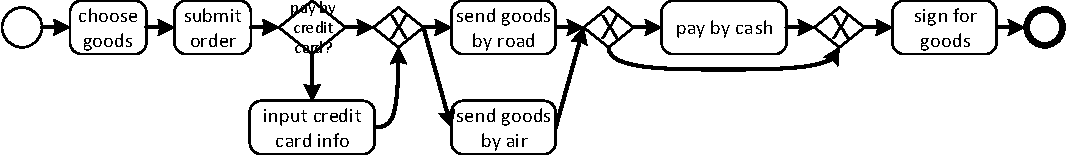
\includegraphics[width=1.0\textwidth]{basic_causal_drawback}
  \caption{含有不同因果关系的在线购物BPMN模型\label{fig:basic_causal_drawback}}
\end{figure}

\begin{example}\label{ex:basic_causal_drawback}
图\ref{fig:basic_causal_drawback}展示了一个在线购物的BPMN模型\footnote{BPMN是一种工作流建模语言,请参见:http://www.bpmn.org/}。在这个模型中,当任务“choose goods”被执行后,任务“submit order”可以被执行,然后任务“send goods by road”和任务“send goods by air”的其中之一可以被执行。显然,任务“choose goods”和任务“submit order”、任务“submit order”和任务“send goods by road”都满足因果关系。然而,这两组因果关系是不完全相同的。当任务“choose goods”被执行后,任务“submit order”一定会被执行而当任务“submit order”被执行后,任务“send goods by road”却不一定会被执行(因为任务“send goods by air”可能被选择执行)。前文提到的基本因果关系不能表达这类不同,所以需要对因果关系进行精炼。
\end{example}

\begin{figure}[htbp]
  \centering
  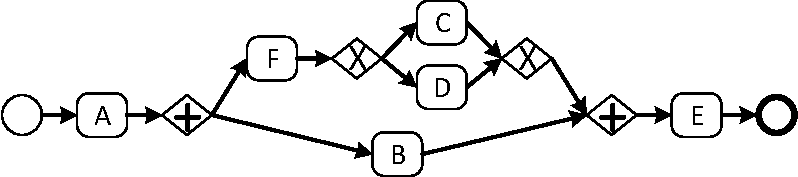
\includegraphics[width=1.0\textwidth]{basic_concurrency_drawback}
  \caption{含有不同并行关系的BPMN模型\label{fig:basic_concurrency_drawback}}
\end{figure}

\begin{example}\label{ex:basic_concurrency_drawback}
图\ref{fig:basic_concurrency_drawback}展示了一个含有并行结构的BPMN模型。在这个模型中,任务“B”和任务“C”可以被并行地执行但当任务“B”被执行时,任务“C”不一定会在同一个执行实例中被执行(因为任务“D”可能被选择执行)。同时,任务“B”和任务“F”也可以被并行地执行而且当任务“B”被执行时,任务“F”一定会在同一个执行实例中被执行。前文提到的基本并行关系不能表达这类不同,所以需要对并行关系进行精炼。
\end{example}

过程模型的任务间不确定性精炼有序关系(以下简称“精炼有序关系”)可以用来刻画过程的行为语义,从而被用于过程模型的检索,即提供一个查询模型$M$和一个过程模型集合$C$,从$C$中查找和$M$行为一致或者最相似的模型。由于本文的方法对过程模型进行了唯一的刻画,所以在检索过程中可以设置不同的粒度以检索符合实际要求的模型。除此之外,精炼有序关系还可以应用于过程模型的符合性检测、相似性度量等领域。

\begin{figure}[htbp]
  \centering
  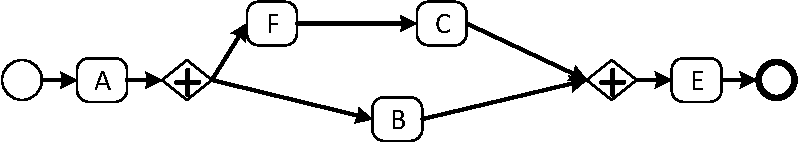
\includegraphics[width=1.0\textwidth]{basic_concurrency_drawback_compare}
  \caption{由图\ref{fig:basic_concurrency_drawback}改造得到的BPMN模型\label{fig:basic_concurrency_drawback_compare}}
\end{figure}

\begin{example}\label{ex:basic_concurrency_drawback_compare}
考虑图\ref{fig:basic_concurrency_drawback}和图\ref{fig:basic_concurrency_drawback_compare}中的模型,当检索满足条件“任务`F'和任务`C'满足因果关系且任务`B'和任务`C'满足并行关系”的模型时,两个模型都符合检索条件。另一方面,将检索条件更改为“任务`F'和任务`C'满足因果关系,且当任务`F'被执行时,任务`C'一定在同一个执行实例中被执行,同时当任务`C'被执行时,任务`F'一定在同一个执行实例中被执行;任务`B'和任务`C'满足并行关系,当任务`B'被执行时,任务`C'一定在同一个执行实例中被执行,同时当任务`C'被执行时,任务`B'一定在同一个执行实例中被执行”时,只有图\ref{fig:basic_concurrency_drawback_compare}中的模型符合条件。显然,精炼后的任务间有序关系能够更加精确地刻画过程模型的行为语义。类似的,这种精炼后的刻画方法可以被当作业务规则用于过程模型的符合性检测。
\end{example}

Jin等人已经提出了一种精炼有序关系RORU及其计算方法\cite{jin2014computing},本文重点对其进行了研究。针对该方法存在的问题,本文提出了改进方案,将新的方法命名为扩展的任务间不确定性精炼有序关系(Extended Refined Ordering Relations with Uncertainty,简称ExRORU)。由于ExRORU是一种刻画过程行为语义的方法,因此在实验过程中,本文将ExRORU与基于行为语义的过程特征刻画算法和过程相似性度量算法进行比较。

\section{预备知识}\label{sec:preliminaries}
本节介绍论文中需要用到的预备知识,其中\ref{subsec:petrinet}介绍Petri网,\ref{subsec:workflow_net}介绍工作流网及相关概念,\ref{subsec:process_run}和\ref{subsec:cpu}分别介绍过程流和完全前缀展开。

\subsection{Petri网}\label{subsec:petrinet}
业务过程建模给业务过程分析人员提供了建立过程模型并分析它们的能力,有许多论著和建模工具对其进行详尽地描述和实现。建模语言是业务过程建模中的核心部分,目前的建模语言包括但不限于:Petri网、EPC(Event-driven process chain,事件驱动过程链)、BPMN(Business Process Model and Notation,业务过程建模符号)、BPEL(Business Process Execution Language,业务过程执行语言)、UML(Unified Modeling Language,统一建模语言)、APROMORE\cite{la2011apromore}。

Petri网是一种有向二分图,于1960年代由Carl Adam Petri发明\cite{petri1962kommunikation},适合于描述含有异步、并发过程的系统。Petri网既有严格的数学表述方式,也有良好的图形化基础。本文使用Petri网作为建模语言,以下概念来自\onlinecite{van2004workflow}。有关Petri网及其性质的详细介绍,请参见\onlinecite{desel2005free,murata1989petri,reisig1998lectures,袁祟义2005petri}。

\begin{definition}[Petri网]\label{def:petrinet}
Petri网是一个三元组$N=(P,T,F)$,其中:
  \begin{itemize}
  	\item[-] $P$是库所的有限集合;
  	\item[-] $T$是变迁的有限集合;
  	\item[-] $P\cap T=\emptyset$且$T\cap P=\emptyset$;
  	\item[-] $F\subseteq(P\times T)\cup(T\times P)$是边的集合。
  \end{itemize}
\end{definition}

\begin{definition}[标识Petri网]\label{def:marked_petrinet}
标识Petri网是一个二元组$(N,s)$,其中$N=(P,T,F)$是一个Petri网,$s:P\rightarrow\mathbb{N}$是一个函数,表示网的标识。所有标识Petri网的集合记作$\mathcal{N}$。
\end{definition}

令$N=(P,T,F)$是一个Petri网。$P\cup T$中的元素称作节点。节点$x$是节点$y$的输入节点,当且仅当$(x,y)\in F$;节点$x$是节点$y$的输出节点,当且仅当$(y,x)\in F$。对于任意节点$x\in P\cup T$,$x$的前集$\bullet x=\{y|(y,x)\in F\}$,$x$的后集$x\bullet=\{y|(x,y)\in F\}$。

\begin{figure}[htbp]
  \centering
  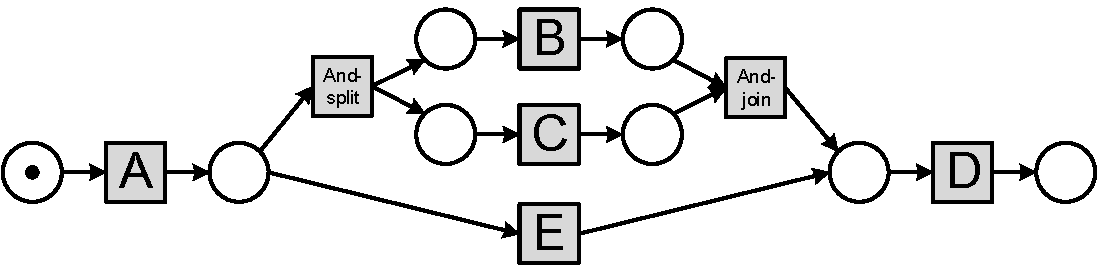
\includegraphics[width=1.0\textwidth]{petri_net_example}
  \caption{标识Petri网示例\label{fig:petri_net_example}}
\end{figure}

图\ref{fig:petri_net_example}展示了一个由8个库所和8个变迁组成的Petri网。变迁$A$有一个输入库所$p_{1}$和一个输出库所$p_{2}$,变迁$AND$-$split$有一个输入库所$p_{2}$和两个输出库所$p_{3}$、$p_{4}$,变迁$AND$-$join$有两个输入库所$p_{5}$、$p_{6}$和一个输出库所$p_{7}$。变迁$A$的输入库所中的黑点表示一个托肯(token),这个托肯即为该Petri网的初始标识。该Petri网的行为由如下发生规则定义。

\begin{definition}[发生规则]\label{def:firing_rule}
令$\Sigma=(N=(P,T,F),s)$是一个标识Petri网:
  \begin{itemize}
  	\item[-] 变迁$t\in T$被使能,记作$(N,s)[t\rangle$,当且仅当$\bullet t\leq s$;
  	\item[-] 发生规则$\_[\_\rangle\_\subseteq\mathcal{N}\times T\times\mathcal{N}$是满足如下条件的最小关系:\\$\forall (N=(P,T,F),s)\in\mathcal{N},\forall t\in T:(N,s)[t\rangle\Rightarrow(N,s)[t\rangle(N,s-\bullet t+t\bullet)$。
  \end{itemize}
\end{definition}

在图\ref{fig:petri_net_example}的标识Petri网(源库所有一个托肯)中,变迁$A$被使能。当变迁$A$发生后,会将其输入库所中的托肯移除,在其输出库所中加入一个托肯,如图\ref{fig:petri_net_example_fire1}所示。此时,变迁$E$和变迁$AND$-$split$都被使能。虽然两者都被使能,但是只有一个能够发生,因为变迁$E$和变迁$AND$-$split$此时会竞争唯一的托肯。如果变迁$AND$-$split$发生,会消耗其输入库所的托肯并在两个输出库所中各生成一个托肯,如图\ref{fig:petri_net_example_fire2}所示。

\begin{figure}[htbp]
  \centering
  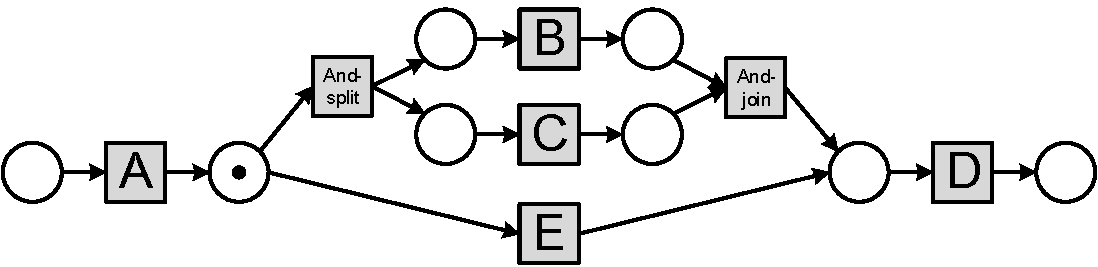
\includegraphics[width=1.0\textwidth]{petri_net_example_fire1}
  \caption{变迁$A$发生后的标识Petri网\label{fig:petri_net_example_fire1}}
\end{figure}

\begin{figure}[htbp]
  \centering
  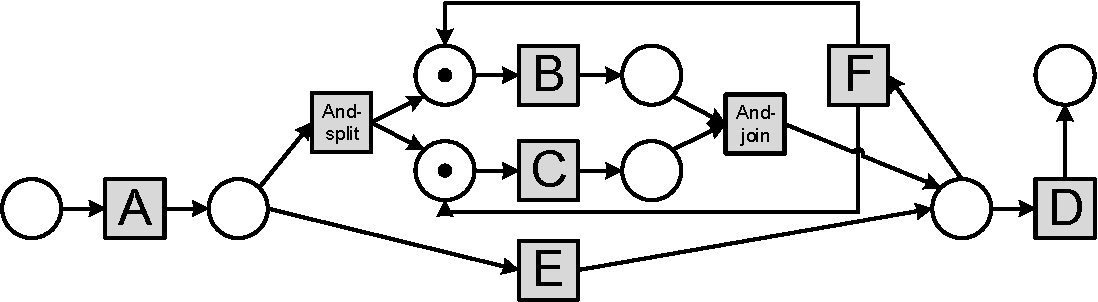
\includegraphics[width=1.0\textwidth]{petri_net_example_fire2}
  \caption{变迁$AND$-$split$发生后的标识Petri网\label{fig:petri_net_example_fire2}}
\end{figure}

\begin{definition}[可达标识]\label{def:reachable_markings}
令$(N,s_{0})\in\mathcal{N}$是一个标识Petri网。标识$s$从初始标识$s_{0}$可达,当且仅当存在一条变迁序列,其变迁依次发生使标识$s_{0}$变为$s$。$(N,s_{0})$所有可达标识的集合记作$[N,s_{0}\rangle$。
\end{definition}

图\ref{fig:petri_net_example}中的标识Petri网有八个可达标识。本文用如下方式描述到达某个可达标识的变迁发生序列。令$A$为标签集合。由$A$内元素组成的长度为$n\in\mathbb{N}$的序列是一个函数$\sigma:\{0,...,n-1\}\rightarrow A$。长度为0的序列称作空序列,记作$\varepsilon$。为了便于理解,一个长度大于0的序列通常简写为函数的值序列。例如,序列$\sigma=\{(0,a),(1,a),(2,b)\}$简写为$aab$。由$A$内元素组成的任意长度的所有序列集合记作$A^{*}$。

\begin{definition}[发生序列]\label{def:firing_sequence}
令$(N=(P,T,F),s_{0})$是一个标识Petri网。序列$\sigma\in T^{*}$是$(N,s_{0})$的一条发生序列当且仅当对于某个自然数$n\in\mathbb{N}$,存在标识$s_{1},...,s_{n}$和变迁$t_{1},...,t_{n}\in T$,使得$\sigma=t_{1}...t_{n}$,且对于所有满足$0\leq i\leq n$的$i$,$(N,s_{i})[t_{i+1}\rangle$且$s_{i+1}=s_{i}-\bullet t_{i+1}+t_{i+1}\bullet$。($n=0$隐含$\sigma=\varepsilon$,$\varepsilon$是$(N,s_{0})$的发生序列。)序列$\sigma$在标识$s_{0}$下可发生,记作$(N,s_{0})[\sigma\rangle$。序列$\sigma$发生后得到标识$s_{n}$,记作$(N,s_{0})[\sigma\rangle(N,s_{n})$。
\end{definition}

\begin{definition}[连通性]\label{def:connectedness}
网$N=(P,T,F)$是弱连通的,或者简称连通的,当且仅当对于任意两个节点$x,y\in P\cup T$,$x(F\cup F^{-1})y$,其中$R^{-1}$是关系$R$的逆,$R^{*}$是关系$R$的自反传递闭包。网$N$是强联通的,当且仅当对于任意两个节点$x,y\in P\cup T$,$xF^{*}y$。
\end{definition}

图\ref{fig:petri_net_example}中的标识Petri网是连通的,但不是强连通的,例如没有从汇库所到源库所的有向路径,也没有从变迁$D$到变迁$A$的有向路径。

\begin{definition}[有界性、安全性]\label{def:boundedness_safeness}
标识Petri网$(N=(P,T,F),s)$是有界的,当且仅当可达标识集合$[N,s\rangle$是有穷的。$(N,s)$是安全的,当且仅当$\forall s'\in[N,s\rangle,\forall p\in P,s.t.~s'(p)\leq 1$。显然,安全性隐含了有界性。
\end{definition}

图\ref{fig:petri_net_example}中的标识Petri网是安全的(也是有界的),因为它的八个可达标识中没有库所会包含超过一个托肯。

\begin{definition}[死变迁,活性]\label{def:dead_transition}
令$(N=(P,T,F),s)$是一个标识Petri网。变迁$t\in T$是死变迁当且仅当$\nexists s'\in[N,s\rangle,s.t.~(N,s')[t\rangle$。$(N,s)$是活的,当且仅当$\forall s'\in[N,s\rangle,\forall t\in T,s.t.~\exists s'\in[N,s'\rangle,(N,s')[t\rangle$。显然,活性隐含不存在死变迁。
\end{definition}

图\ref{fig:petri_net_example}中的标识Petri网的所有变迁都不是死变迁。但是它不是活的,因为它无法使每个变迁不断地发生。

\subsection{工作流网}\label{subsec:workflow_net}
大多数工作流系统提供了构建标准逻辑的连接语义词,例如$AND$-$split$,$AND$-$join$,$OR$-$split$和$OR$-$join$\cite{van2004workflowbook,fischer2002workflow,jablonski1996workflow,leymann2000production}。这些语义词被用于建模顺序、条件、并行和循环结构\cite{fischer2002workflow}。显然,Petri网拥有足够的能力来表达上述结构:用变迁表示任务,库所和边表示因果依赖。例如,库所可以表示任务的前驱条件或者后继条件;$AND$-$split$可以用含有多个输出库所的变迁表示;$OR$-$split$/$OR$-$join$可以用含有多条出边/入边的库所表示。

用于建模工作流中控制流维度的Petri网称作工作流网(Workflow net,缩写为WF-net)。工作流网最先由荷兰教授Wil M.P. van der Aalst提出\cite{van1998application}。

\begin{definition}[工作流网]\label{def:workflow_net}
令$N=(P,T,F)$是一个Petri网,$\overline{t}$是不属于$P\cup T$的新节点。$N$是工作流网(WF-net)当且仅当:
  \begin{itemize}
  	\item[-] 对象创建:$P$含有一个输入库所$i$满足:$\bullet i=\emptyset$;
  	\item[-] 对象完成:$P$含有一个输出库所$o$满足:$o\bullet=\emptyset$;
  	\item[-] 连通性:$\overline{N}=(P,T\cup\{\overline{t}\},F\cup\{(o,\overline{t}),(\overline{t},i)\})$是强连通的。
  \end{itemize}
\end{definition}

图\ref{fig:petri_net_example}中的标识Petri网是一个WF-net。虽然该网不是强连通的,但其短回路网$\overline{N}=(P,T\cup\{\overline{t}\},F\cup\{(o,\overline{t}),(\overline{t},i)\})$是强连通的。即使一个网满足定义\ref{def:workflow_net}中的所有条件,其对应的过程模型仍然可能包含诸如死锁、永远不被使能的任务、活锁、过程终止后有残留托肯等错误。因此,需要定义如下原则。

\begin{definition}[合理性]\label{def:sound}
令$N=(P,T,F)$为一个WF-net,其输入库所为$i$,输出库所为$o$。$N$是合理的,当且仅当:
  \begin{itemize}
  	\item[-] 安全性:$(N,[i])$是安全的;
  	\item[-] 恰当完成:$\forall s\in[N,[i]\rangle,s.t.~o\in s\Rightarrow s=[o]$;
  	\item[-] 可完成:$\forall s\in[N,[i]\rangle,s.t.~[o]\in[N,s\rangle$;
  	\item[-] 不含死任务:$(N,[i])$不包含死变迁。
  \end{itemize}
所有合理的WF-net组成集合$\mathcal{W}$。
\end{definition}

图\ref{fig:petri_net_example}中的WF-net是合理的。合理性可以用标准Petri网分析技术来验证。事实上,WF-net的合理性对应于其短回路网的活性和安全性\cite{van1997verification,van1998application,van2004workflowbook}。因此,可以应用高效的算法和工具验证WF-net的合理性,例如针对WF-net的裁剪分析工具Woflan\cite{verbeek2001diagnosing}。

\subsection{过程流}\label{subsec:process_run}
本文针对过程模型的任务间有序关系进行精炼,首先给出有序关系的标准定义。

\begin{definition}[任务间有序关系\cite{esparza2002improvement}]\label{def:ordering_relations}
Petri网的任意一对节点$x,y$之间有三种基本有序关系:
  \begin{itemize}
  	\item[-] $x$和$y$满足因果关系,当且仅当该网存在一条至少包含一条边、从$x$到$y$的路径,记作$x<y$;
  	\item[-] $x$和$y$满足冲突关系,当且仅当该网存在两条开始于同一个库所$s$的路径$st_{1}...x$和$st_{2}...y$,且$t_{1}...x$和$t_{2}...y$不相交,记作$x\#y$;
  	\item[-] $x$和$y$满足并行关系,当且仅当$x$和$y$既不满足因果关系,也不满足冲突关系,记作$x~co~y$。
  \end{itemize}
\end{definition}

如前文所述,本文对因果关系和并行关系进行精炼。为了便于定义与描述,本文使用过程流来描述仅含有上述两种关系的模型。使用过程流可以恰当地描述变迁发生序列中的因果和并行关系。一个网系统的过程流是一种称作因果网的特殊网,并使用一个函数将因果网的节点映射到原网系统的节点上。

\begin{definition}[因果网\cite{polyvyanyy20144c}]\label{def:causal_net}
$N=(B,E,G)$是因果网,当且仅当:
  \begin{itemize}
  	\item[-] 对于任意$b\in B$,满足:$|\bullet b|\leq 1$且$|b\bullet|\leq 1$;
  	\item[-] $N$是无环的,即$G^{+}$是非自反的。
  \end{itemize}
\end{definition}

$B$和$E$中的元素分别称为$N$的条件和事件。因果网$N=(B,E,G)$的两个节点$x$和$y$满足因果关系,当且仅当$(x,y)\in G^{+}$;$x$和$y$满足并行关系,当且仅当$x\neq y$,$(x,y)\notin G^{+}$且$(y,x)\notin G^{+}$。一个因果网的割是其所有俩俩并行条件的最大集合。

因果网的事件可以用来描述变迁发生序列。

\begin{definition}[过程流\cite{polyvyanyy20144c}]\label{def:process_run}
标识Petri网$(N=(P,T,F),s)$的过程流是一个有序二元组$\pi=(N_{\pi},\rho)$,其中$N_{\pi}=(B,E,G)$是一个因果网,$\rho:B\cup E\rightarrow P\cup T$是一个映射函数且满足如下条件:
  \begin{itemize}
  	\item[-] $\rho(B)\subseteq P$且$\rho(E)\subseteq T$;
  	\item[-] $Min(N_{\pi})$是一个割且$\forall p\in P:s(p)=|\rho^{-1}(p)\cap Min(N_{\pi})|$,即$\pi$的初始标识是$s$;
  	\item[-] 对于任意事件$e\in E$和任意库所$p\in P$满足:$\bm{1}_{F}((p,\rho(e)))=|\rho^{-1}(p)\cap\bullet e|$且$\bm{1}_{F}((\rho(e),p))=|\rho^{-1}(p)\cap e\bullet|$.\footnote{$\bm{1}_{F}$表示$F$在集合$(P\times T)\cup(T\times P)$上的特征函数。}
  \end{itemize}
\end{definition}

给定一个过程流$\pi$,事件集合$E$和映射函数$\rho$经常被记作$E_{\pi}$和$\rho_{\pi}$。一个标识Petri网$S$所有过程流的集合记作$\Pi_{S}$。前文提到的因果关系和并行关系同样可以定义在$\pi$的因果网节点上,分别记作$\rightarrowtail_{\pi}$和$\parallel{\pi}$,在含义明确的情况下脚标常被省略。

\begin{figure}[htbp]
  \centering
  \begin{subfigure}{1\textwidth}
  	\centering
  	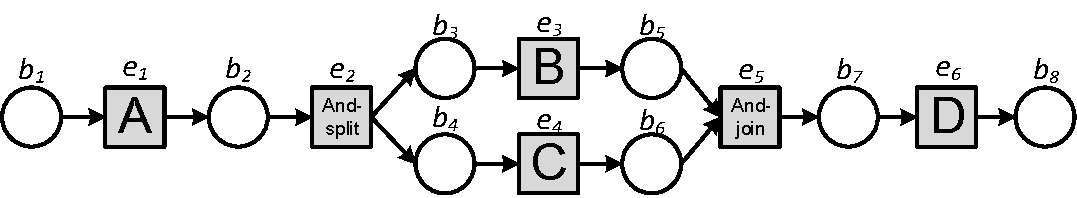
\includegraphics[width=0.65\textwidth]{process_run_example_1}
  	\caption{\label{fig:process_run_example_1}}
  \end{subfigure}
  \begin{subfigure}{1\textwidth}
  	\vspace{1em}
  	\centering
  	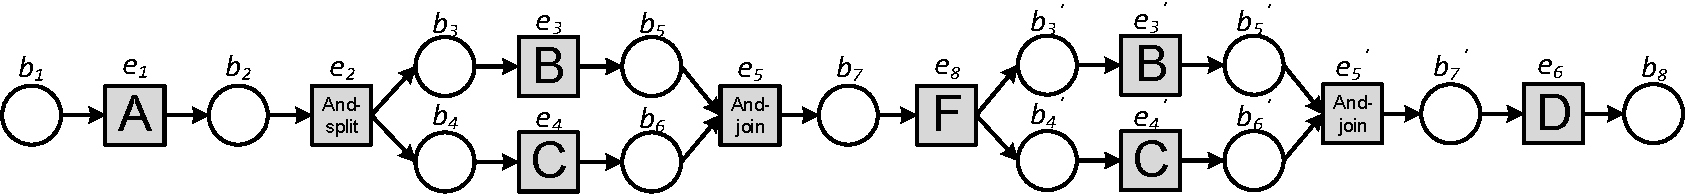
\includegraphics[width=1\textwidth]{process_run_example_2}
  	\caption{\label{fig:process_run_example_2}}
  \end{subfigure}
  \caption{图\ref{fig:petri_net_example}中模型的两个过程流示例}
\end{figure}

图\ref{fig:process_run_example_1}和图\ref{fig:process_run_example_2}展示了图\ref{fig:petri_net_example}中模型的两个过程流$\pi_{1}$和$\pi_{2}$。当对过程流进行图形化展示时,条件$c_{i},c_{i}'...$对应于库所$p_{i}$,即$\rho(c_{i})=\rho(c_{i}')=p_{i}$。类似的,事件$e_{j},e_{j}'...$对应于变迁$t_{j}$,即$\rho(e_{j})=\rho(e_{j}')=t_{j}$。在图\ref{fig:process_run_example_2}中,$e_{3}\parallel e_{4}$、$e_{4}\rightarrow e_{4}'$、$e_{3}'\parallel e_{4}'$。显然,若两个事件在一个Petri网$N$的过程流$\pi$中满足因果关系,则它们在原网中对应的变迁必然能在某个变迁发生序列中顺序发生。类似的,若两个事件在$\pi$中满足并行关系,则它们在原网中对应的变迁必然会在某个可达标识$s$下同时被使能,而且可以在$s$这个标识下以任意顺序发生。

每个事件$e\in E_{\pi}$都代表着对应变迁$\rho_{\pi}(e)$的一次发生。J{\"o}rg Desel等人给出了一个网系统的过程流与其变迁发生序列对应的方法\cite{desel2000validation}。给定一个Petri网,对其过程流加标识得到$(N_{\pi},s)$,其中$N_{\pi}$是该网过程流$(N_{\pi},\rho)$的因果网且标识$s$仅在每个源条件中放置一个托肯。通过映射函数$\rho$可以将该过程流的事件发生序列与原网的变迁发生序列对应起来。例如,图\ref{fig:process_run_example_1}中的过程流的事件发生序列可以对应图\ref{fig:petri_net_example}中模型的变迁发生序列$t_{1}t_{2}t_{3}t_{4}t_{5}t_{6}$。

\subsection{完全前缀展开}\label{subsec:cpu}
在一个模型的所有过程流中,只有因果关系和并行关系被抽取出来。因此,在一个过程流中只存在顺序和并发结构,而不存在循环和互斥结构。然而,由于过程模型中循环结构的存在,一个模型可能有无穷多个过程流,区别在于循环结构展开的程度。显然,使用这无穷多个过程流去抽取ExRORU是不现实的。Javier Esparza等人提出了完全前缀展开(Complete Prefix Unfolding,简称CPU)的概念来避免此问题\cite{esparza2002improvement}。

考虑一个含有根节点的有向图$G$。众所周知该图可以被展开成一棵带有标签的树(树的节点正好是图$G$中从根节点开始的所有路径上的点)。树上的节点标签由图中的节点决定。上述展开过程可以在任意时间停止,从而得到不同的树。显然,如果尽可能多地将图展开,总会得到一棵唯一的标签树,通常是无穷大的。这棵最大的树称为该图的展开(unfolding)。

类似的,Petri网也可以被展开成带标签的发生网(occurrence nets,是一种带有类树型结构的简单图)。发生网的节点标签由原网的库所和标签决定。通过一个Petri网展开得到的发生网被称作分支过程(branching processes)。展开过程可以在任意时间停止,从而得到不同的分支过程。显然,如果尽可能多地将Petri网展开,总会得到一个唯一的分支过程,通常是无穷大的。这个最大的分支过程称为该Petri网的展开。

\begin{definition}[发生网]\label{def:occurrence_net}
发生网$O=(B,E,F)$是满足如下条件的网:
  \begin{enumerate}[(1)]
  	\item $\forall b\in B,|\bullet b|\leq 1$;
  	\item $O$是无环网,或者说该网的因果关系是一种偏序关系;
  	\item $O$是有穷前驱的,即,对于任意节点$x\in B\cup E$,满足$y<x$的元素$y\in B\cup E$的集合是有穷的;
  	\item 没有元素与自身冲突。
  \end{enumerate}
\end{definition}

显然,发生网中的任意两个节点间正好满足定义\ref{def:ordering_relations}中的三种关系之一。$B$和$E$中的元素通常被称为条件和事件。$Min(O)$表示$B\cup E$中前集为空的元素集合。由于在合理WF-net中所有的变迁前集都不为空,所以$Min(O)$中的元素只有条件。

\begin{definition}[分支过程]\label{def:branching_process}
标识Petri网$\Sigma=(P,T,F,s_{0})$的分支过程是一个标签发生网$\beta=(O,p)=(B,E,F,p)$,其中函数$p$满足如下性质:
  \begin{enumerate}[(i)]
  	\item $p(B)\subseteq P$且$p(E)\subseteq T$($p$保持了节点的本性);
  	\item 对于任意$e\in E$,函数$p$对于$\bullet e$的约束是一个从$\bullet e$($\sigma$中)到$\bullet p(e)$($\beta$中)的双射,$e\bullet$和$p(e)\bullet$类似($p$保持了标签的环境);
  	\item 函数$p$对$Min(O)$的约束是一个从$Min(O)$到$s_{0}$的双射($\beta$从$s_{0}$“开始”);
  	\item $\forall e_{1},e_{2}\in E:\bullet e_{1}=\bullet e_{2}\wedge p(e_{1})=p(e_{2})\Rightarrow e_{1}=e_{2}$($\beta$不会重复$\Sigma$中的变迁)。
  \end{enumerate}
\end{definition}

\begin{figure}[htbp]
  \centering
  \begin{subfigure}{1\textwidth}
  	\centering
  	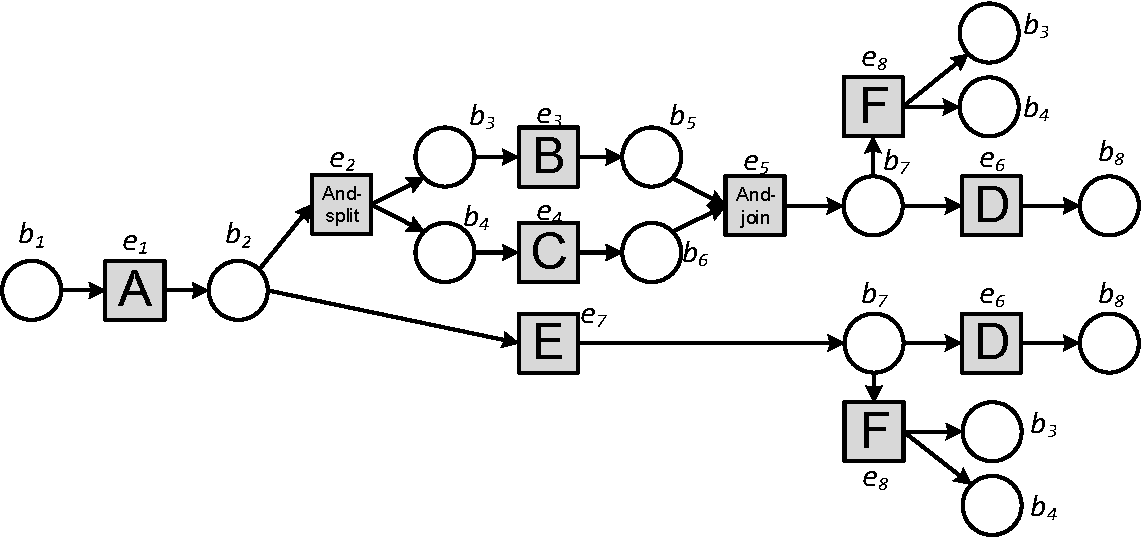
\includegraphics[width=0.7\textwidth]{branching_process_example_1}
  	\caption{\label{fig:branching_process_example_1}}
  \end{subfigure}
  \begin{subfigure}{1\textwidth}
  	\vspace{1em}
  	\centering
  	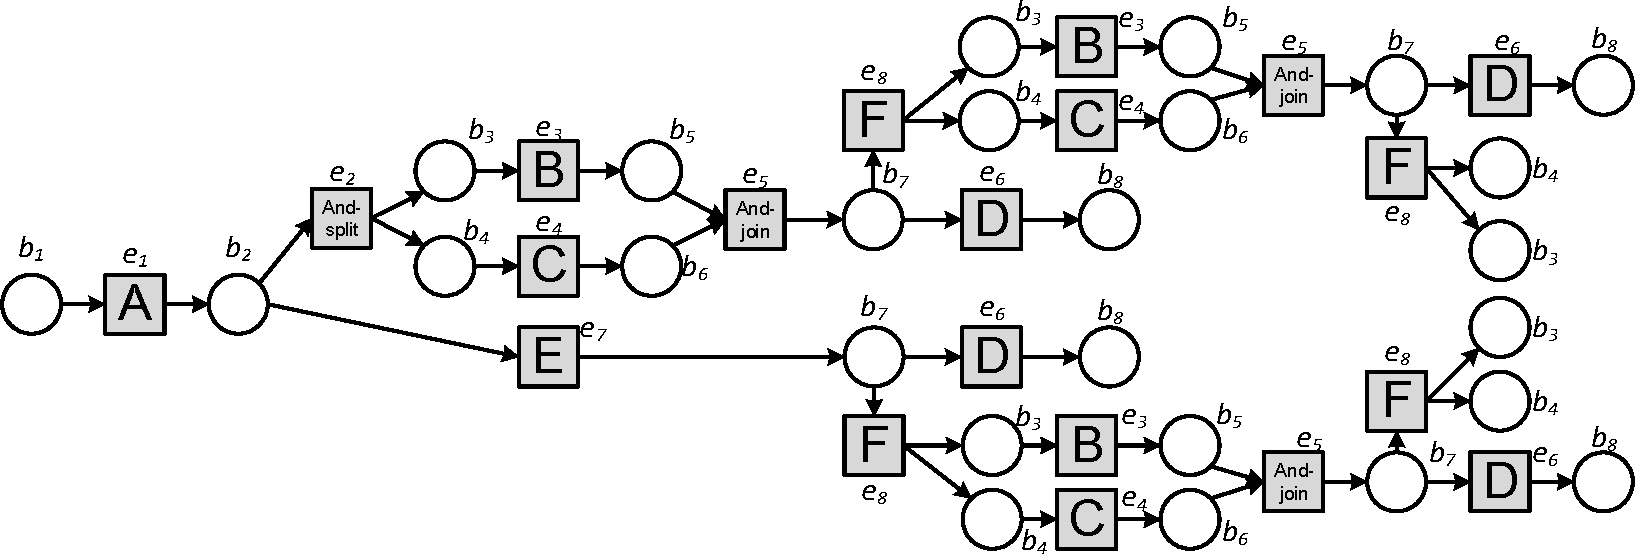
\includegraphics[width=1\textwidth]{branching_process_example_2}
  	\caption{\label{fig:branching_process_example_2}}
  \end{subfigure}
  \caption{图\ref{fig:petri_net_example}中模型的两个分支过程}
  \label{fig:branching_process_example}
\end{figure}

图\ref{fig:branching_process_example_1}和图\ref{fig:branching_process_example_2}展示了图\ref{fig:petri_net_example}中模型的两个分支过程。分支过程的差别在于它们展开的程度,展开少的分支过程是那些展开的多的分支过程的前缀。

\begin{definition}[分支过程前缀]\label{def:branching_process_prefix}
令$\beta'=(O',p')$和$\beta=(O,p)$是一个标识Petri网的两个分支过程。$\beta'$是$\beta$的前缀,当且仅当$O'$是$O$的子图且满足如下条件:
  \begin{itemize}
  	\item[-] $Min(O)$属于$O'$;
  	\item[-] 如果条件$b$属于$O'$,那么它在$O$中的输入事件$e\in\bullet b$也属于$O'$(如果存在的话);
  	\item[-] 如果事件$e$属于$O'$,那么它在$O$中的输入和输出条件$\bullet e\cup e\bullet$也属于$O'$。
  \end{itemize}
  $p'$是函数$p$在$O'$上的对应。
\end{definition}

根据上述前缀定义,一个Petri网总有一个唯一的最大分支过程\cite{engelfriet1991branching},即前文所述的Petri网展开。图\ref{fig:petri_net_example}中模型的展开是无穷大的。

一个分支过程有一个自然的初始标识,即在每个源条件内放置一个托肯。据此,可以形式化一个展开如何描述Petri网的行为:令$\Sigma$是一个标识Petri网,$\beta$是它的展开。$\Sigma$和$\beta$的可达图有着同构化的展开形式。$\Sigma$的可达标识就是满足$s$是$\beta$的可达标识的那些$p(s)$;对于$\beta$的一个可达标识$s$和$\Sigma$的可达标识$s''$、变迁$t$,存在可达标识$s'$和事件$e$满足$p(s')=s''$,$p(e)=t$且$s\overset{e}{\rightarrow}s'$当且仅当在$\Sigma$中$p(s)\overset{t}{\rightarrow}s''$成立。

\begin{definition}[完全前缀展开,CPU]\label{def:cpu}
令$O=(B,E,A,p)$是一个发生网,其中$p$是发生网节点到原始标识Petri网节点的多对一映射,$e\in E$是任意事件。
  \begin{itemize}
  	\item[-] 事件$e$的局部配置$\lceil e\rceil$是在$e$之前可达$e$的事件集合;
  	\item[-] 局部配置$\lceil e\rceil$的终结标识$Mark(\lceil e\rceil)$是在$\lceil e\rceil$中事件都被触发后被标识的事件集合;
  	\item[-] 充分顺序$\prec$是定义在局部配置上的严格有根据的偏序关系,满足$\lceil e\rceil\subset\lceil e'\rceil\Rightarrow\lceil e\rceil\prec\lceil e'\rceil\Rightarrow$\footnote{这里使用了\onlinecite{esparza2002improvement}中在1-安全Petri网上定义的完全顺序关系。};
  	\item[-] 事件$e$被称为截断事件,当且仅当存在一个关联事件$e'$满足$Mark(\lceil e\rceil)=Mark(\lceil e'\rceil)$且$\lceil e'\rceil\prec\lceil e\rceil$;
  	\item[-] 完全前缀展开是一个发生网的最大后向闭包子图,且在截断事件后没有任何事件。
  \end{itemize}
\end{definition}

\begin{figure}[htbp]
  \centering
  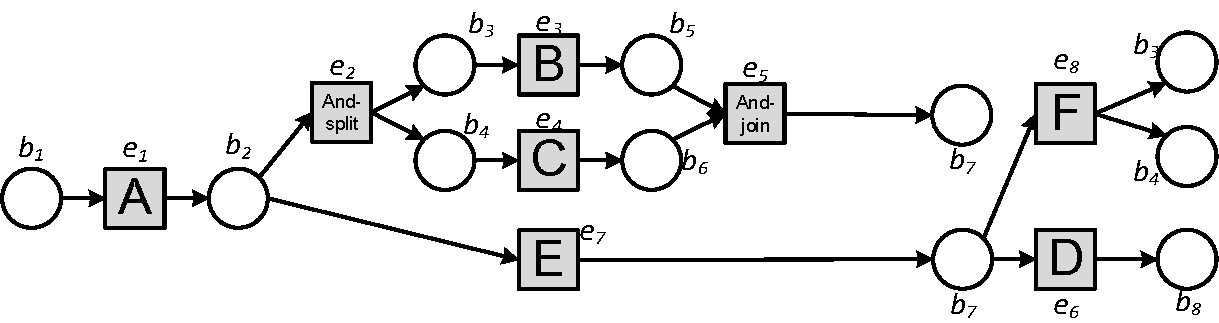
\includegraphics[width=1\textwidth]{cpu_example}
  \caption{图\ref{fig:petri_net_example}中模型的CPU\label{fig:cpu_example}}
\end{figure}

图\ref{fig:cpu_example}展示了图\ref{fig:petri_net_example}中模型的CPU。在该CPU中,事件$AND$-$join$和事件$F$是截断事件。事件$AND$-$join$的关联事件是$E$,$F$的关联事件是$AND$-$split$。

显然,将一个模型的CPU从截断事件后面继续展开可以得到这个模型的所有过程流。换句话说,CPU是一个模型最小但最完整的过程流表达。因此,本文使用过程流来定义所有的关系,并使用CPU来高效计算它们。

\section{当前面临的挑战}\label{sec:challenge}
本文主要工作在于对RORU算法的扩展上,因此有必要探讨原算法所面临的挑战。本文之所以选择RORU作为研究基础,一方面是因为它是定义在被广泛使用的WF-net上,有很多成熟的建模和分析工具可以利用,且其算法能被扩展到使用各种语言建模的过程模型中;另一方面,RORU对过程行为语义进行了细致的刻画,且给出了高效、准确的计算方法。本小节只简单列举RORU的部分不足之处,更详细的讨论会在本文后续章节中涉及。本文提出的ExRORU同样定义在WF-net上,但是与RORU相似,其思路可以被扩展到使用各种语言建模的过程模型中。

{\heiti 循环结构。}正如\onlinecite{jin2014computing}所述,RORU算法针对无环过程模型。然而实际生活中,大约10\%-20\%都是含有循环结构的。所以RORU对于环处理的缺失会大大降低其能力。

{\heiti 不可见任务。}不可见任务是指过程模型中存在,但是实际执行日志中并不存在的任务。RORU将不可见任务也作为普通可见任务处理,然而过程模型中可能存在充当路由功能的无意义任务。另外,在变迁发生序列中信息的缺失和噪声的存在都可能导致挖掘过程产生不可见任务。目前,RORU并没有考虑不可见任务对过程模型行为的影响,所以无法正确处理含有不可见任务的模型。

{\heiti 非自由选择结构。}为了还原过程模型两个变迁之间的关系,需要将其CPU中对应事件的关系进行映射。在含有非自由选择结构的过程模型的CPU中会出现重名事件,导致事件间的关系不唯一。RORU并未考虑重名事件的影响。

{\heiti 紧邻关系。}上述两种结构的存在会使得一些结构上并不紧邻的事件在事件发生序列中紧邻发生,从而影响其行为语义。RORU未考虑事件间紧邻关系的存在,故对一些行为相似但不一致的模型无法区分。

本文重点对以上不足之处进行改进,探讨如何应对这些挑战。

\section{论文的主要贡献}\label{sec:contribution}
本文尝试对RORU算法\cite{jin2014computing}的不足进行扩展,主要有以下几点贡献:
\begin{enumerate}[1.]
  \item 提出了扩展不确定性精炼任务间关系,即ExRORU。利用ExRORU可以刻画所有类型的合理过程模型,包括含有循环结构、不可见任务及非自由选择结构的模型。
  \item 探讨ExRORU如何能识别任意一堆过程模型之间的行为差异,即给出一个过程模型行为语义的唯一刻画。
  \item 给出ExRORU算法的实现并在效率、能力和可扩展性上将其与现有的计算任务间关系的主流算法进行比较。
\end{enumerate}

\section{论文章节安排}\label{sec:structure}
本文章节安排如下,第\ref{cha:intro}章对全文进行概述,介绍本文选题背景和意义、涉及到的基本知识以及当前算法所面临的主要挑战,从而引出本文的工作重点。第\ref{cha:related_work}主要介绍过程模型行为刻画方法的研究现状,分类介绍了国内外学者提出的各类算法并分析其优缺点,尤其重点介绍了本文基础RORU算法的处理能力和不足之处。第\ref{cha:exroru}章详细阐述了ExRORU的定义和计算方法,并探讨了其检测任意一对过程模型行为差异的能力,并重点分析了事件间ExRORU和变迁间ExRORU关系的相互关系。第\ref{cha:experiment}章给出了ExRORU算法的实现并将其与现有的计算任务间关系的主流算法进行了比较,此外还重点将其与RORU进行了效率、能力等方面的对比。第\ref{cha:conclusion}章对本文工作进行总结并对未来工作进行了展望。
\chapter{相关工作}\label{cha:related_work}
本章将重点介绍现有的刻画过程模型行为语义的算法,同时对本文改进的RORU算法进行介绍和分析。

\section{过程模型行为语义刻画方法}\label{sec:related_algorithms}
国内外学者提出了诸多刻画过程模型行为语义的方法与工具,它们的适用场景和刻画能力各有不同。对过程模型行为语义的刻画可以应用到过程模型相似性度量方法及过程模型差异性检测中,本节重点介绍部分主流过程模型行为语义刻画方法和基于过程模型行为特征的相似性度量算法。

Zha等人基于两个模型的变迁发生序列集提出了一种简单的相似性度量方法,即参考相似性算法(reference similarity)\cite{zha2010workflow}。作者同时给出了此方法的两个严重问题:首先,该方法不适用于带环模型,因为带环模型的变迁发生序列是无穷多的;其次,该方法过于严格,现实中存在发生序列相似但无完全相同序列的模型对,该类模型对会被认为完全不相似。

基于上述原因,Zha等人又提出了另一种相似性算法,即TAR算法(Trasition adjacency relation,变迁紧邻关系)。一对变迁$A,B$被认为是$TAR$集合中的元素当且仅当模型存在一条形如$\langle ...,A,B,...\rangle$的变迁发生序列,即变迁$A$后面紧跟着变迁$B$。令模型$M_{0}$和模型$M_{1}$的$TAR$关系集合分别是$TAR_{0}$和$TAR_{1}$,则两个模型间的$TAR$相似度被定义为$sim(M_{0},M_{1})=(\#(TAR_{0}\cap TAR_{1})/\#(TAR_{0}\cup TAR_{1}))$。因为模型$M_{0}$和$M_{1}$中的变迁数量是有限的,所以$TAR_{0}$和$TAR_{1}$是有穷的。作者同时证明了该算法对应的距离度量是度量空间中的距离函数。

TAR相似性算法解决了带环WF-net的相似性度量问题,是一种基于过程模型行为特征的相似性算法。但是TAR算法只考虑了变迁之间的直接紧邻关系,而忽略了变迁紧邻关系之间的传递闭包。该算法只考虑了“变迁$A$后可以被变迁$B$直接跟随”,而没有考虑“变迁$A$发生后,变迁$B$可以在之后某个时候发生”。该缺陷导致算法不能对循环结构与顺序结构对应的紧邻关系进行区分,影响度量结果。此外,TAR算法也不能正确处理带有非自由选择结构的过程模型。

Weidlich等人通过抽取两个变迁执行之间的依赖关系刻画一个过程模型的行为语义\cite{weidlich2011efficient,weidlich2010efficient}。变迁之间的依赖关系被分成四类:
\begin{itemize}
  \item[-] 变迁$A$和变迁$B$满足严格顺序关系(strict order relation),当且仅当变迁$A$可能在变迁$B$之前被执行,而变迁$B$不可能在变迁$A$之前被执行,即存在形如$\langle ...A...B...\rangle$的变迁发生序列而不存在形如$\langle ...B...A...\rangle$的变迁发生序列。
  \item[-] 变迁$A$和变迁$B$满足互斥关系(exclusiveness relation),当且仅当变迁$A$和变迁$B$不可能在同一个变迁发生序列中同时出现。
  \item[-] 变迁$A$和变迁$B$满足观察并行关系(observation concurrency relation)(\onlinecite{weidlich2011efficient}中称之为交错顺序关系(interleaving order relation)),当且仅当变迁$A$可能在变迁$B$之前被执行,变迁$B$也可能在变迁$A$之前被执行。
  \item[-] 变迁$A$和变迁$B$满足共现关系(co-occurrence relation),当且仅当在每个变迁$A$出现的变迁发生序列中,变迁$B$也被执行。
\end{itemize}
上述四种关系被称为因果行为轮廓(causal behavioural profile,简称CBP)。

为了比较模型$M_{0}$和模型$M_{1}$的行为,首先需要为两个模型的变迁之间建立一个映射关系,该映射关系由一个相关关系$\sim$表示。关系$\sim$满足$M_{0}$可以与$M_{1}$的多个点对应,反之亦然。

Weidlich等人基于如下思想定义了一种相似性度量方法(\onlinecite{weidlich2011efficient,weidlich2010efficient}中称之为一致性程度):对于一个模型中每对变迁,如果在另一个模型中有对应的变迁对(由关系$\sim$决定),就检查这两个模型对是否满足相同的关系(严格顺序、互斥、交错顺序、共现)。

形式化的,令$T_{0}$和$T_{1}$分别为模型$M_{0}$和模型$M_{1}$的变迁集。定义$T_{0}^{\sim}=\{a\in T_{0}:\exists b\in T_{1},\text{s.t.}~a\sim b\}$以及$T_{1}^{\sim}=\{b\in T_{1}:\exists a\in T_{0},\text{s.t.}~a\sim b\}$。因为存在一对多的映射,所以$T_{0}^{\sim}$的大小与$T_{1}^{\sim}$不一定一致。一致性变迁对集合$C_{0}\subseteq T_{0}^{\sim}\times T_{0}^{\sim}$是所有满足如下条件的变迁对$(x_{0},y_{0})\in T_{0}^{\sim}\times T_{0}^{\sim}$:对于所有满足$x_{0}\sim x_{1}$且$y_{0}\sim y_{1}$的变迁对$(x_{1},y_{1})\in T_{1}^{\sim}\times T_{1}^{\sim}$,$x_{0}$和$y_{0}$有着与$x_{1}$和$y_{1}$相同的关系。同理定义一致性变迁对集合$C_{1}\subseteq T_{1}^{\sim}\times T_{1}^{\sim}$。

基于上述定义,可以用如下公式计算相似性(被称为一致性度量):
\begin{displaymath}
  sim(M_{0},M_{1})=\frac{\#C_{0}+\#C_{1}}{\#(T_{0}^{\sim}\times T_{0}^{\sim})+\#(T_{1}^{\sim}\times T_{1}^{\sim})}
\end{displaymath}

CBP可以被应用于模型检索和一致性检测。作者给出了一个高效计算过程模型因果行为轮廓的算法\cite{weidlich2010efficient},但该算法只适用于合理的自由选择WF-net。此外,在部分模型中,CBP不能区分循环结构和并行结构,所以拥有相同CBP的两个模型可能有着不同的行为。

Dijkman等人提出了因果足迹(causal footprints,简称CF)算法来抽取过程模型变迁之间的前驱关系\cite{dijkman2011similarity}。假定过程模型的变迁集合为$T$,它的因果足迹是一个二元组$(L_{lb},L_{la})$。该二元组的第一个元素$L_{lb}\subseteq (\wp(T)\times T)$被称为后向链接集合,$(S,a)\in L_{lb}$当且仅当在某个变迁发生序列中每次变迁$a$的发生都有变迁集合$S$中某个变迁的发生作为其前驱。同理,$L_{la}$被称为前向链接集合,$(T\times\wp(T))\supseteq(a,S)\in L_{la}$当且仅当在某个变迁发生序列中每次变迁$a$的发生都有变迁集合$S$中某个变迁的发生作为其后继。

为了度量两个模型间的相似性,需要计算它们的因果足迹之间的相似性。CF被当作文档向量空间中的文档,这是在信息过滤和信息检索领域中被广泛使用的一个概念\cite{salton1975vector}。因果足迹(“文档”)被表示成索引项的向量。假定模型$M_{0}=(N_{0},E_{0})$和$M_{1}=(N_{1},E_{1})$的前向链接集合分别为$L_{la}^{M_{0}}$和$L_{la}^{M_{1}}$,后向链接集合分别为$L_{lb}^{M_{0}}$和$L_{lb}^{M_{1}}$。索引项集合$\Uptheta=N_{0}\cup N_{1}\cup L_{la}^{M_{0}}\cup L_{la}^{M_{1}}\cup L_{lb}^{M_{0}}\cup L_{lb}^{M_{1}}$,即$\Uptheta$包含了两个模型的所有节点及所有的前向链接和后向链接。令$\lambda:\Uptheta\rightarrow\mathbb{N}$是一个索引函数,它给每个索引项赋予一个递增数字。

模型$M_{i}$($i\in\{0,1\}$)被表示成向量$\vec{g^{i}}=(g_{1}^{i},g_{2}^{i},...,g_{\#\Uptheta}^{i})$。\onlinecite{van2008measuring}给出了其取值:
\begin{displaymath}
  g{_{\lambda(t)}^i}=
    \begin{cases}
        0& if\quad t\notin N_i\cup L{_{la}^{M_i}}\cup L{_{lb}^{M_i}}\\
        1& if\quad t\in N_i\\
        \frac{1}{2^{len(t)}-1}& if\quad t\in L{_{la}^{M_i}}\cup L{_{lb}^{M_i}}
    \end{cases}
\end{displaymath}
其中$len(t)$是前向链接集合或者后向链接集合中元素的个数。模型$M_{0}$和模型$M_{1}$的相似度用两个模型的向量夹角余弦值表示:
\begin{displaymath}
  sim(M_{0},M_{1})=\frac{\vec{g^{0}}\times\vec{g^{1}}}{\vec{g^{0}}\cdot\vec{g^{1}}}
\end{displaymath}

CF的最大缺点在于$L_{la}$和$L_{lb}$含有大量的无用元素\cite{dijkman2011similarity,van2008measuring}。由于该方法使用的向量空间维度很高,因此向量的计算效率很低。另外,CF算法不区分$OR$连接和$XOR$连接,从而影响计算结果的合理性。

为了解决带环模型变迁发生序列集合无穷大的问题,Wang等人通过限制子序列来度量相似性:一条不含重复变迁的发生序列被看作一个整体来处理\cite{wang2010behavioral}。该算法被称为主变迁序列(principle transition sequences,简称PTS)。含有重复变迁$x$的序列$\sigma$被表达为$\sigma=\langle\sigma_{prefix},x,\sigma_{repeatable},x,...\rangle$,其中$\sigma_{prefix}$和$\sigma_{repeatable}$是$\sigma$的子序列。如此,在计算过程中,子序列$\sigma_{prefix}$和$\sigma_{repeatable}$会替代$\sigma$来参与计算。作者证明了对于每个过程模型,子序列的数量是有限的。

基于最长公共子序列可以定义两个子序列之间的相似性:
\begin{displaymath}
  sim_{trace}(\sigma_{1},\sigma_{2})=\frac{len(lcs(\sigma_{1},\sigma_{2}))}{max(len(\sigma_{1}),len(\sigma_{2}))}
\end{displaymath}
假定模型$M_{0}$和模型$M_{1}$的变迁集分别为$T_{0}$和$T_{1}$,基于上述子序列相似性可以得到模型相似性公式如下:
\begin{displaymath}
  sim(M_{0},M_{1})=\frac{\sum_{\sigma\in T_{0}}\text{max}_{\sigma'\in T_{1}}sim_{trace}(\sigma,\sigma')+\sum_{\sigma'\in T_{1}}\text{max}_{\sigma\in T_{0}}sim_{trace}(\sigma',\sigma)}{\#T_{0}+\#T_{1}}
\end{displaymath}

PTS算法对变迁发生序列集合的相似性计算较为粗糙,未考虑子序列基数差异的影响,且其只使用最大相似度来衡量集合间的相似性,计算结果不够精确。另一方面,当处理含有高并发结构的过程模型时,PTS算法存在状态空间爆炸的问题。

作为对PTS算法的改进,Dong等人提出了基于触发序列集合的过程模型相似性算法,即CFS(全称complete firing sequences)\cite{dong2014cfs}。相比于PTS,CFS算法引入了循环计数的概念从而避免计算所有触发序列。CFS算法使用过程模型的覆盖树来计算触发序列集合,通过比较两个过程模型的触发序列集合来衡量两者的相似性。与PTS类似,作者首先定义了触发序列之间的相似性:
\begin{displaymath}
  sims(\sigma,\sigma')=\frac{length(lcs(L(\sigma),L(\sigma')))}{max(length(L(\sigma)),length(L(\sigma')))}
\end{displaymath}
在度量触发序列集合之间的相似性时,CFS不仅考虑了集合元素间的相似度,还考虑了两集合的基数差异。令$A$,$B$是两个完整触发序列集合,不失一般性假定$|A|\leq|B|$,令$\text{avg}(A,\sigma')=\frac{\sum_{\sigma\in A}sims(\sigma,\sigma')}{|A|}$表示完整触发序列集合$A$与单一完整触发序列$\sigma$的相似度,$\text{dis}(A,B)=\frac{||A|-|B||}{|B|}$表示$A$和$B$的基数距离。同时,令$M:A\rightarrow B$为一个单射,它将$A$中的完整触发序列映射到$B$中的序列,令$B'=B-\text{cod}(M)$,$n$为正整数,则$A$与$B$的相似度公式定义为:
\begin{displaymath}
  simc(A,B)=\frac{\sum_{(\sigma,\sigma')\in M}sims(\sigma,\sigma')+\sum_{\sigma'\in B'}\text{avg}(A,\sigma')}{|B|}\times(1-\frac{\text{dis}(A,B)}{n})
\end{displaymath}
并将此作为两个过程模型间的相似度。作者同时给出了利用贪心算法和$A^{*}$算法求解完整触发序列集合间最优映射的方法。与PTS类似,基于覆盖树的CFS算法也存在状态空间爆炸的问题。

Artem Polyvyanyy等人定义了Petri网的4C频谱(共现co-occurrence、冲突conflict、因果causality和并行concurrency)并据此刻画模型的行为语义\cite{polyvyanyy20144c}。作者首先探讨了冲突和共现关系,任意一种刻画变迁的发生之间关联情况的关系都可以被归纳成以下两种情况之一:两个变迁是否能在同一个发生序列中同时出现;一个变迁是否可以在某个其他变迁不发生的情况发生。基于此作者给出基本冲突和基本共现的定义:
\begin{definition}[基本冲突和基本共现]
令$S=(N=(P,T,F),M)$是一个标识Petri网,$x,y\in T$是其两个变迁。
  \begin{itemize}
    \item[-] $x$与$y$可以冲突,当且仅当$S$中存在一个变迁发生序列$\sigma$使得$x\in\sigma$且$y\notin\sigma$,记作$x\dashedrightarrow_{S}y$;
    \item[-] $x$与$y$可以共现,当且仅当$S$中存在一个变迁发生序列$\sigma$使得$x\in\sigma$且$y\in\sigma$,记作$x\leftrightharpoonupdown_{S}y$。\footnote{给定一个变迁发生序列$\sigma$,$x\in\sigma$表示$x$在$\sigma$中出现。}
  \end{itemize}
\end{definition}
在含义明确的情况脚标常被省略。借用析取范式和合取范式的概念作者进一步给出了4C频谱中的冲突和共现定义:
\begin{definition}[冲突和共现]
令$S=(N=(P,T,F),M)$是一个标识Petri网,$x,y\in T$是其两个变迁。
  \begin{itemize}
    \item[-] $x$与$y$共现,当且仅当$\overline{x\dashedrightarrow_{S}y}\wedge\overline{y\dashedrightarrow_{S}x}\wedge x\leftrightharpoonupdown_{S}y$,记作$x\leftrightarrow_{S}y$;
    \item[-] $x$与$y$冲突,当且仅当$x\dashedrightarrow_{S}y\wedge y\dashedrightarrow_{S}x\wedge\overline{x\leftrightharpoonupdown_{S}y}$,记作$x\#_{S}y$;
    \item[-] $x$需要$y$,当且仅当$\overline{x\dashedrightarrow_{S}y}\wedge y\dashedrightarrow_{S}x\wedge x\leftrightharpoonupdown_{S}y$,记作$x\rightharpoonup_{S}y$;
    \item[-] $x$与$y$相互独立,当且仅当$x\dashedrightarrow_{S}y\wedge y\dashedrightarrow_{S}x\wedge x\leftrightharpoonupdown_{S}y$,记作$x\rightleftharpoons_{S}y$。
  \end{itemize}
\end{definition}
除此之外还有两种与死变迁相关的合取范式:
\begin{definition}[不发生]
令$S=(N=(P,T,F),M)$是一个标识Petri网,$x,y\in T$是其两个变迁。
  \begin{itemize}
    \item[-] $x$与$y$从不发生,当且仅当$\overline{x\dashedrightarrow_{S}y}\wedge\overline{y\dashedrightarrow_{S}x}\wedge\overline{x\leftrightharpoonupdown_{S}y}$,记作$x\mid_{S}y$;
    \item[-] $x$发生但$y$不发生,当且仅当$x\dashedrightarrow_{S}y\wedge\overline{y\dashedrightarrow_{S}x}\wedge\overline{x\leftrightharpoonupdown_{S}y}$,记作$x\vdash_{S}y$。
  \end{itemize}
\end{definition}
综上得到冲突和共现关系的频谱:
\begin{definition}[冲突和共现关系的频谱]\label{def:spectrum_of_conflict_cooccurence}
令$S=(N=(P,T,F),M)$是一个标识Petri网,$x,y\in T$是其两个变迁。$\Omega$是一个由原子命题$x\dashedrightarrow_{S}y$、$y\dashedrightarrow_{S}x$和$x\leftrightharpoonupdown_{S}y$组成的命题范式。
  \begin{itemize}
    \item[-] $\Omega$描述$x$和$y$之间的冲突关系当且仅当$\Omega$的完美3DNF的每个合取范式含有$x\dashedrightarrow_{S}y$或者$y\dashedrightarrow_{S}x$;
    \item[-] $\Omega$描述$x$和$y$之间的共现关系当且仅当$\Omega$的完美3DNF的每个合取范式含有$x\leftrightharpoonupdown_{S}y$。
  \end{itemize}
\end{definition}
给定网$S$,分别用$\diamondtimes_{S}$和$\diamondplus_{S}$表示$S$中所有的冲突和共现关系。给定两个变迁$x$和$y$,共有四种合取范式包含了原子$x\leftrightharpoonupdown y$:(1)$x\dashedrightarrow y\wedge y\dashedrightarrow x\wedge x\leftrightharpoonupdown y$;(2)$\overline{x\dashedrightarrow y}\wedge y\dashedrightarrow x\wedge x\leftrightharpoonupdown y$;(3)$\overline{x\dashedrightarrow y}\wedge y\dashedrightarrow x\wedge x\leftrightharpoonupdown y$;(4)$\overline{x\dashedrightarrow y}\wedge\overline{y\dashedrightarrow x}\wedge x\leftrightharpoonupdown y$。因此,共有$2^{4}-1$,即15中不同的共现关系,每种共现关系都是一个或者多个上述合取范式的析取范式。同理,共有63中不同的冲突关系。

之后,作者开始探讨因果和并行关系。给定两个变迁$x$和$y$,对于因果和并行关系的分类建立在三个维度上:(1)关系是否在模型的部分或者全部过程流中成立;(2)关系是否在一个或者全部含有$x$的过程流中成立;(3)关系是否在一个或者全部含有$y$的过程流中成立。为了便于理解,首先给出一个能选择出描述$x$和$y$发生情况的过程流的过滤器:$\Delta_{S}(x,y)=\{\pi\in\Pi_{S}|\exists e_{1}\in E_{\pi}\exists e_{2}\in E_{\pi}:e_{1}\neq e_{2}\wedge\rho_{\pi}(e_{1})=x\wedge\rho_{\pi}(e_{2})=y\}$。为了检查两个变迁在所有包含它们的过程流中的并行模式,作者定义了完全并行关系。
\begin{definition}[完全并行]\label{def:total_concurrency}
令$S=(N=(P,T,F),M)$是一个标识Petri网,$x,y\in T$是其两个变迁。
  \begin{itemize}[leftmargin=22pt]
    \item[-] $x$和$y$满足完全(相互)并行关系,记作$x\parallel_{S}^{\forall\forall\forall}y$,当且仅当\\
    $
      \forall\pi\in\Delta_{S}(x,y)\forall e_{1}\in E_{\pi}\forall e_{2}\in E_{\pi}:(e_{1}\neq e_{2}\wedge\rho_{\pi}(e_{1})=x\wedge\rho_{\pi}(e_{2})=y)\Rightarrow e_{1}\parallel_{\pi}e_{2}
    $;
    \item[-] $x$对于$y$满足完全功能并行关系,记作$x\parallel_{S}^{\forall\forall\exists}y$,当且仅当\\
    $
      \forall\pi\in\Delta_{S}(x,y)\forall e_{1}\in E_{\pi}\exists e_{2}\in E_{\pi}:\rho(e_{1})=x\Rightarrow(\rho_{\pi}(e_{2})\wedge e_{1}\parallel_{\pi}e_{2})
    $;
    \item[-] $x$对于$y$满足完全支配并行关系,记作$x\parallel_{S}^{\forall\exists\forall}y$,当且仅当\\
    $
      \forall\pi\in\Delta_{S}(x,y)\exists e_{1}\in E_{\pi}\forall e_{2}\in E_{\pi}:\rho_{\pi}(e_{1})=x\wedge((\rho_{\pi}(e_{2})=y\wedge e_{1}\neq e_{2})\Rightarrow e_{1}\parallel_{\pi}e_{2})
    $;
    \item[-] $x$与$y$满足完全存在并行关系,记作$x\parallel_{S}^{\forall\exists\exists}y$,当且仅当\\
    $
      \forall\pi\in\Delta_{S}(x,y)\exists e_{1}\in E_{\pi}\exists e_{2}\in E_{\pi}:\rho_{\pi}(e_{1})=x\wedge\rho_{\pi}(e_{2})=y\wedge e_{1}\parallel_{\pi}e_{2}
    $。
  \end{itemize}
\end{definition}
为了检查两个变迁在至少一个包含它们的过程流中的并行模式,作者定义了存在并行关系。
\begin{definition}[存在并行]\label{def:existential_concurrency}
令$S=(N=(P,T,F),M)$是一个标识Petri网,$x,y\in T$是其两个变迁。
  \begin{itemize}[leftmargin=22pt]
    \item[-] $x$和$y$满足存在完全并行关系,记作$x\parallel_{S}^{\exists\forall\forall}y$,当且仅当\\
    $
      \exists\pi\in\Delta_{S}(x,y)\forall e_{1}\in E_{\pi}\forall e_{2}\in E_{\pi}:(e_{1}\neq e_{2}\wedge\rho_{\pi}(e_{1})=x\wedge\rho_{\pi}(e_{2})=y)\Rightarrow e_{1}\parallel_{\pi}e_{2}
    $;
    \item[-] $x$对于$y$满足存在功能并行关系,记作$x\parallel_{S}^{\exists\forall\exists}y$,当且仅当\\
    $
      \exists\pi\in\Delta_{S}(x,y)\forall e_{1}\in E_{\pi}\exists e_{2}\in E_{\pi}:\rho(e_{1})=x\Rightarrow(\rho_{\pi}(e_{2})\wedge e_{1}\parallel_{\pi}e_{2})
    $;
    \item[-] $x$对于$y$满足存在支配并行关系,记作$x\parallel_{S}^{\exists\exists\forall}y$,当且仅当\\
    $
      \exists\pi\in\Delta_{S}(x,y)\exists e_{1}\in E_{\pi}\forall e_{2}\in E_{\pi}:\rho_{\pi}(e_{1})=x\wedge((\rho_{\pi}(e_{2})=y\wedge e_{1}\neq e_{2})\Rightarrow e_{1}\parallel_{\pi}e_{2})
    $;
    \item[-] $x$与$y$满足存在(完全)并行关系,记作$x\parallel_{S}^{\exists\exists\exists}y$,当且仅当\\
    $
      \exists\pi\in\Delta_{S}(x,y)\exists e_{1}\in E_{\pi}\exists e_{2}\in E_{\pi}:\rho_{\pi}(e_{1})=x\wedge\rho_{\pi}(e_{2})=y\wedge e_{1}\parallel_{\pi}e_{2}
    $。
  \end{itemize}
\end{definition}
将定义\ref{def:total_concurrency}和定义\ref{def:existential_concurrency}中的$e_{1}\parallel_{\pi}e_{2}$替换成$e_{1}\rightarrowtail_{\pi}e_{2}$就得到了完全因果关系和存在因果关系的定义。

令$\Phi=\{\forall\forall\forall,\forall\forall\exists,\forall\exists\forall,\forall\exists\exists,\exists\forall\forall,\exists\forall\exists,\exists\exists\forall,\exists\exists\exists\}$,因果和并行关系的频谱定义如下:
\begin{definition}[因果和并行关系的频谱]\label{def:spectrum_of_causality_concurrency}
令$S=(N=(P,T,F),M)$是一个标识Petri网,$x,y\in T$是其两个变迁。
  \begin{itemize}
    \item[-] $x$和$y$满足因果关系,记作$x\rightarrowtail_{S,\diamonddot}^{\phi}y$,当且仅当\\
    $(x\diamonddot_{S}y)\wedge(x\rightarrowtail_{S}^{\phi}y)$,其中$\diamonddot_{S}\in\diamondplus_{S}$,$\phi\in\Phi$;
    \item[-] $x$和$y$满足并行关系,记作$x\parallel_{S,\diamonddot}^{\phi}y$,当且仅当\\
    $(x\diamonddot_{S}y)\wedge(x\parallel_{S}^{\phi}y)$,其中$\diamonddot_{S}\in\diamondplus_{S}$,$\phi\in\Phi$。
  \end{itemize}
\end{definition}
定义\ref{def:spectrum_of_causality_concurrency}可以推导出$15\times 8=120$中不同的因果关系和相同数量的并行关系。定义\ref{def:spectrum_of_conflict_cooccurence}和定义\ref{def:spectrum_of_causality_concurrency}共同组成了变迁之间行为关系的4C频谱。

4C频谱是一种完整且基本的关系定义,但是作者在\onlinecite{polyvyanyy20144c}中只给出了其中四种关系的计算方法。此外,存在两个拥有相同4C频谱关系但有着不同行为语义的模型\cite{armas2014suitability}。

\section{精炼不确定性有序关系}\label{sec:roru}
既然本文主要工作是对RORU算法的改进,有必要对\onlinecite{jin2014computing}中的RORU算法进行介绍。首先定义$\Sigma=(P,T,F,M_{0})$是标识Petri网,$\beta=(B,E,A,f)$是$\Sigma$的分支过程,$x,y,a,b,c\in E$都是$\beta$的事件。一条路径指分支过程中从开始状态到终止状态的一条有向路径。

基于一个任务是否总是和另一个任务在同一个执行实例中被执行,因果关系可以被精炼成以下四种。其中C是Certain的简写,U是Uncertain的简写。

\begin{definition}[确定-确定因果,简称C-C因果]\label{def:c_c_causal}
$x$和$y$满足CC因果关系,记作$x\twoheadrightarrow y$,当且仅当:
  \begin{itemize}
    \item[-] $x$和$y$满足因果关系,即$x<y$;
    \item[-] 如果$x$出现在一条路径上,$y$必须之后也出现在这条路径上;
    \item[-] 如果$y$出现在一条路径上,$x$必须之前也出现在这条路径上;
  \end{itemize}
\end{definition}

\begin{definition}[确定-不确定因果,简称C-U因果]\label{def:c_u_causal}
$x$和$y$满足CU因果关系,记作$x\rightharpoonup y$,当且仅当:
  \begin{itemize}
    \item[-] $x$和$y$满足因果关系,即$x<y$;
    \item[-] 如果$x$出现在一条路径上,$y$可能之后不出现在这条路径上;
    \item[-] 如果$y$出现在一条路径上,$x$必须之前也出现在这条路径上;
  \end{itemize}
\end{definition}

\begin{definition}[不确定-确定因果,简称U-C因果]\label{def:u_c_causal}
$x$和$y$满足UC因果关系,记作$x\mapsto y$,当且仅当:
  \begin{itemize}
    \item[-] $x$和$y$满足因果关系,即$x<y$;
    \item[-] 如果$x$出现在一条路径上,$y$必须之后也出现在这条路径上;
    \item[-] 如果$y$出现在一条路径上,$x$可能之前不出现在这条路径上;
  \end{itemize}
\end{definition}

\begin{definition}[不确定-不确定因果,简称U-U因果]\label{def:u_u_causal}
$x$和$y$满足UU因果关系,记作$x\rightleftharpoons y$,当且仅当:
  \begin{itemize}
    \item[-] $x$和$y$满足因果关系,即$x<y$;
    \item[-] 如果$x$出现在一条路径上,$y$可能之后不出现在这条路径上;
    \item[-] 如果$y$出现在一条路径上,$x$可能之前不出现在这条路径上;
  \end{itemize}
\end{definition}

类似地,可以将并行关系也精炼为以下四种。

\begin{definition}[确定-确定并行,简称C-C并行]\label{def:c_c_concurrency}
$x$和$y$满足CC并行关系,记作$x\equiv y$,当且仅当:
  \begin{itemize}
    \item[-] $x$和$y$满足并行关系,即$x~co~y$;
    \item[-] 如果$x$被执行,$y$必须也在同一个实例中被执行;
    \item[-] 如果$y$被执行,$x$必须也在同一个实例中被执行;
  \end{itemize}
\end{definition}

\begin{definition}[确定-不确定并行,简称C-U并行]\label{def:c_u_concurrency}
$x$和$y$满足CU并行关系,记作$x\Downarrow y$,当且仅当:
  \begin{itemize}
    \item[-] $x$和$y$满足并行关系,即$x~co~y$;
    \item[-] 如果$x$被执行,$y$必须也在同一个实例中被执行;
    \item[-] 如果$y$被执行,$x$可能不在同一个实例中被执行;
  \end{itemize}
\end{definition}

\begin{definition}[不确定-确定并行,简称U-C并行]\label{def:u_c_concurrency}
$x$和$y$满足UC并行关系,记作$x\Uparrow y$,当且仅当:
  \begin{itemize}
    \item[-] $x$和$y$满足并行关系,即$x~co~y$;
    \item[-] 如果$x$被执行,$y$可能不在同一个实例中被执行;
    \item[-] 如果$y$被执行,$x$必须也在同一个实例中被执行;
  \end{itemize}
\end{definition}

\begin{definition}[不确定-不确定并行,简称U-U并行]\label{def:u_u_concurrency}
$x$和$y$满足UU并行关系,记作$x\Updownarrow y$,当且仅当:
  \begin{itemize}
    \item[-] $x$和$y$满足并行关系,即$x~co~y$;
    \item[-] 如果$x$被执行,$y$可能不在同一个实例中被执行;
    \item[-] 如果$y$被执行,$x$可能不在同一个实例中被执行;
  \end{itemize}
\end{definition}

之后,作者提出一些用于紧邻任务计算的基本规则和用于非紧邻任务计算的传递性规则,并基于此给出了一个基于CPU计算无环过程模型RORU的算法。RORU有着一些明显的缺点,不能被应用于实际企业中。

\begin{figure}[htbp]
  \centering
  \subcaptionbox{\label{fig:sda_example_1}}{
    \centering
    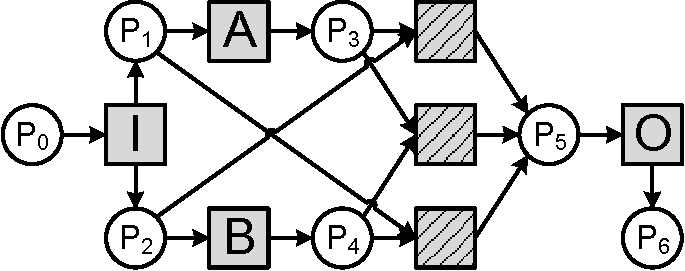
\includegraphics[width=0.45\textwidth]{sda_example_1}
  }
  \hspace{1em}
  \subcaptionbox{\label{fig:sda_example_2}}{
    \centering
    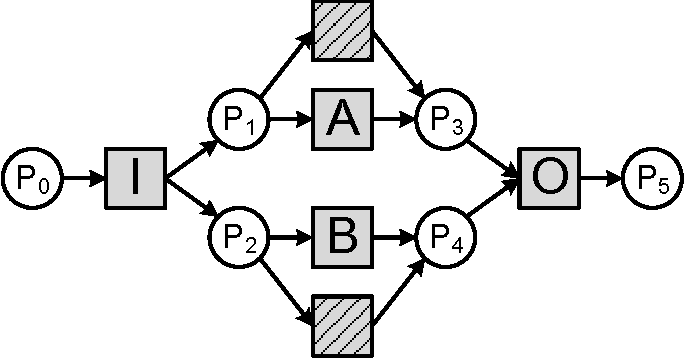
\includegraphics[width=0.45\textwidth]{sda_example_2}
  }
  \caption{RORU无法区分的一对含有不可见变迁的模型}
  \label{fig:sda_example}
\end{figure}

首先,RORU不能被应用于带环的WF-net,这已经在\onlinecite{jin2014computing}的标题中明确指出。其次,由于RORU没有考虑不可见变迁,变迁发生序列中的发生顺序紧邻但模型结构上不紧邻的变迁无法被区分,所以两个有着不同行为语义的WF-net可能会被混淆。例如,图\ref{fig:sda_example_1}中WF-net的变迁发生序列集合是$\{\langle I,A,B,O\rangle,\langle I,B,A,O\rangle,\langle I,A,O\rangle,\langle I,B,O\rangle\}$而图\ref{fig:sda_example_2}中WF-net的变迁发生序列集合是$\{\langle I,A,B,O\rangle,\langle I,B,A,O\rangle,\langle I,A,O\rangle,\langle I,B,O\rangle,\langle I,O\rangle\}$。显然,这两个WF-net的行为是不一致的,但是RORU不能区分它们。

\begin{figure}[htbp]
  \centering
  \subcaptionbox{\label{fig:nfc_example_1}}{
    \centering
    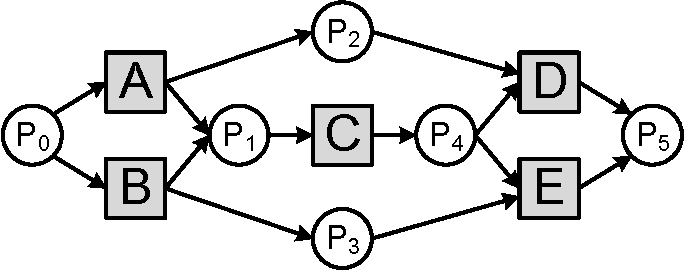
\includegraphics[width=0.45\textwidth]{nfc_example_1}
  }
  \hspace{1em}
  \subcaptionbox{\label{fig:nfc_example_2}}{
    \centering
    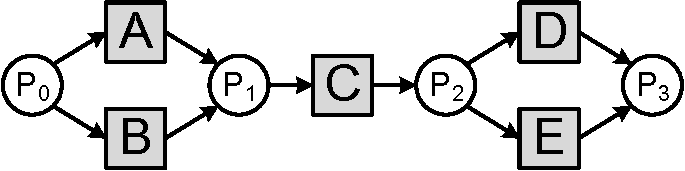
\includegraphics[width=0.45\textwidth]{nfc_example_2}
  }
  \caption{RORU无法区分的一对含有非自由选择结构的模型}
  \label{fig:nfc_example}
\end{figure}

在一个含有非自由选择结构\cite{de2003workflow}的WF-net中,变迁之间的因果关系不一定满足传递性。以图\ref{fig:nfc_example_1}和图\ref{fig:nfc_example_2}中的模型为例,变迁$A$和变迁$C$满足因果关系,变迁$C$和变迁$E$亦满足因果关系。根据RORU的传递性规则,变迁$A$和变迁$E$应满足因果关系。然而,这在图\ref{fig:nfc_example_1}含有非自由选择结构的WF-net中是不正确的,因为当变迁$A$首先被执行后,只有变迁$C$和变迁$D$(而不是变迁$E$)可以被执行。因此,变迁$A$和变迁$E$永远不会满足因果关系。

为了解决上述RORU存在的问题,本文将RORU中的有序关系进一步扩展,从而得到一个更为精细的方法去区分任意两个过程模型的行为语义。除了细化原算法的不确定性概念之外,本文引入了任务间多关系的概念,即一对任务之间可能含有不止一种关系。多关系概念的引入可以检测两个过程模型间更为细微的差异。

\section{本章小结}
本章首先对过程模型行为语义刻画算法的国内外研究现状进行了简要介绍和分析,选取了TAR、BP、CF、PTS、CFS、4C等算法为例并分析了它们的优缺点。本章随后对本文工作的基础RORU算法进行了详细的介绍并探讨了其缺陷。
\chapter{扩展不确定性精炼有序关系及其计算}\label{cha:exroru}
\section{ExRORU算法概述}\label{sec:exroru_intro}
本章主要介绍基于扩展不确定性精炼有序关系的过程模型行为语义刻画方法,即ExRORU算法(Extended Refined Ordering Relations with Uncertainty)。ExRORU算法主要包含两部分工作:一是基于CPU抽取事件间的ExRORU关系,二是将事件间的ExRORU关系折叠得到WF-net变迁之间的ExRORU关系。本章重点介绍ExRORU的计算方法,其计算过程如图\ref{fig:exroru_procedure}所示。

\begin{figure}[htbp]
  \centering
  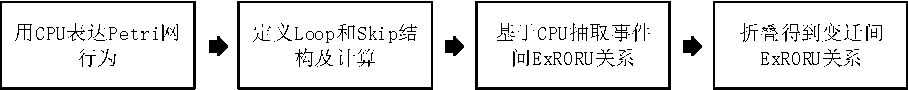
\includegraphics[width=1.0\textwidth]{exroru_procedure}
  \caption{ExRORU算法的基本流程\label{fig:exroru_procedure}}
\end{figure}

\textcolor{red}{
ExRORU计算步骤如下:
\begin{enumerate}[1.]
  \item 计算CPU。依据定义\ref{def:cpu},构造给定合理WF-net的CPU。
  \item 抽取事件间ExRORU关系。
\end{enumerate}
}

\section{ExRORU定义}\label{sec:exroru_definition}
本节主要介绍ExRORU的定义,首先介绍事件间的扩展不确定性精炼因果关系和并行关系,随后介绍变迁间的ExRORU关系。方便起见,约定$\Sigma=(P,T,F,M_{0})$是一个合理WF-net,$U=(B,E,A,f)$是其CPU。令$x,y\in E$是$U$的两个事件。示例WF-net及其CPU如图\ref{fig:case_study_petri}和图\ref{fig:case_study_cpu}所示。

\begin{figure}[htbp]
  \centering
  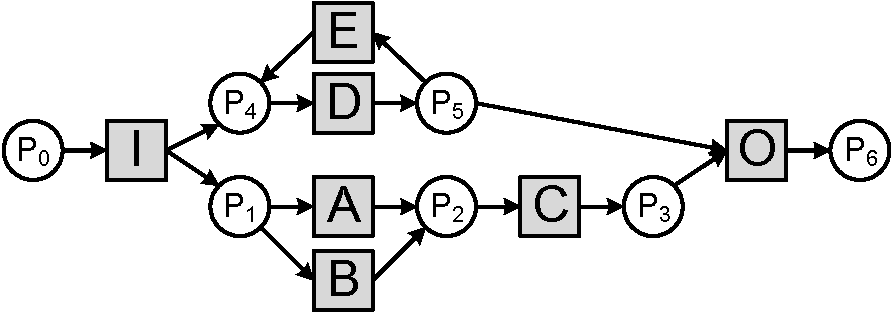
\includegraphics[width=0.7\textwidth]{case_study_petri}
  \caption{一个合理WF-net\label{fig:case_study_petri}}
\end{figure}

\begin{figure}[htbp]
  \centering
  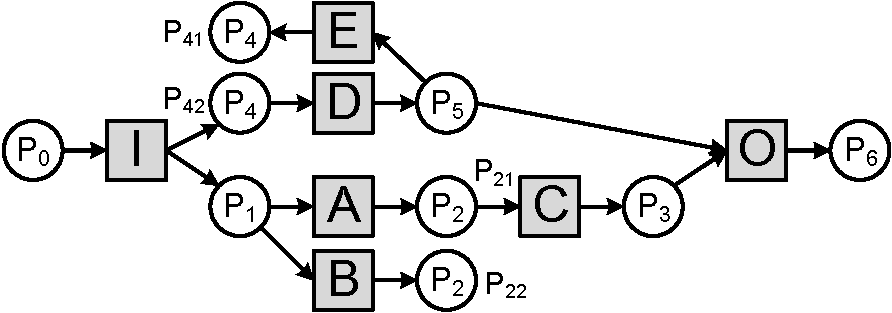
\includegraphics[width=0.7\textwidth]{case_study_cpu}
  \caption{图\ref{fig:case_study_petri}的CPU\label{fig:case_study_cpu}}
\end{figure}

\subsection{事件间扩展不确定性精炼因果关系}\label{subsec:exroru_causal}
本文用形如$[ab\{c,d\}e]$的表达式来描述过程流的行为语义。连续出现的字母表示处于顺序结构中的事件;大括号中的表达式表示并行结构,其不同分支用逗号隔开。该表达式可以互相嵌套以表达复杂过程流的语义。例如在图\ref{fig:case_study_cpu}的CPU中,$[I\{D,AC\}O]$、$[I\{D,BC\}O]$和$[I\{DED,AC\}O]$是一些过程流表达式示例。

轨迹是一系列事件的有穷序列$\sigma\in E^{*}$,可以从网的初始状态开始按顺序执行其中的事件最终得到终止状态。令$\Omega$是$U$中所有过程流的轨迹集合。不可见事件/变迁是模型中起路由作用的无意义事件/变迁,在逻辑流中不被表达出来\cite{wen2007mining}。本文使用带斜线的阴影方框表示不可见事件/变迁,如图\ref{fig:sda_example}所示。基于两个事件是否能在一条轨迹中紧邻发生,首先定义直接和简介因果关系。

\begin{definition}[直接和间接因果关系]\label{def:d_i_causal_relation}
事件$x$和$y$满足因果关系,即$x<y$。它们满足直接因果关系当且仅当:$\exists\sigma=\langle e_{1},e_{2},...,e_{n}\rangle\in\Omega,1\leq i<j\leq n,e_{i}=x,e_{j}=y$,使得$\forall k\in(i,j)$,$e_{k}$是不可见事件。否则,$x$和$y$满足间接因果关系。
\end{definition}

\begin{example}\label{ex:sda}
在图\ref{fig:case_study_cpu}的CPU中,事件$A$和$C$、事件$C$和$O$都满足直接因果关系而事件$A$和$O$满足间接因果关系。
\end{example}

令$\Uptheta$是经$U$展开得到的所有过程流集合,$\Uptheta_{x}$是$\Uptheta$中含有$x$的过程流子集,即$\Uptheta_{x}=\{\beta\in\Uptheta|x\in\beta\}$。$TS(\beta)$表示过程流$\beta$所有轨迹的集合。

\begin{definition}[事件间扩展不确定性精炼因果关系]\label{def:exroru_causal}
事件$x$和$y$满足:
  \begin{itemize}
  	\item[-] 总是因果关系(always causal relation),记作$x\overset{\text{\tiny{A}}}{\rightarrow}y$,当且仅当:$x<y$且$\forall\beta_{x}\in\Uptheta_{x}$,$\forall\sigma\in TS(\beta_{x})$:在$x$被执行后,$y$必须被执行且在每两个$x$的执行之间(如果$\sigma$中有超过一个$x$)至少有一个$y$要被执行。
  	\item[-] 从不因果关系(never causal relation),记作$x\overset{\text{\tiny{N}}}{\rightarrow}y$,当且仅当:$\forall\beta_{x}\in\Uptheta_{x}$,$\forall\sigma\in TS(\beta_{x})$:当$x$被执行,$y$不能在其后被执行。
  	\item[-] 有时因果关系(sometimes causal relation),记作记作$x\overset{\text{\tiny{S}}}{\rightarrow}y$,当且仅当$x$和$y$不满足上述两种关系。
  \end{itemize}
进一步,如果$x$和$y$满足直接因果关系,则$x\overset{\text{\tiny{DA}}}{\rightarrow}y$或者$x\overset{\text{\tiny{DS}}}{\rightarrow}y$(“$D$”表示“direct”);否则$x\overset{\text{\tiny{IA}}}{\rightarrow}y$或者$x\overset{\text{\tiny{IS}}}{\rightarrow}y$(“$I$”表示“indirect”)。
\end{definition}

以上定义的关系统称扩展不确定性精炼因果关系(extened refined causal relation with uncertainty),用$\rightarrow$表示。显然,满足“从不因果关系”的两个事件是无需区分其是否满足“直接因果关系”的。

\begin{example}\label{ex:exroru_causal}
在图\ref{fig:case_study_cpu}的CPU中,事件$A$和事件$C$满足“直接总是因果关系”(direct always causal relation),即$A\overset{\text{\tiny{DA}}}{\rightarrow}C$,因为在所有含有事件$A$的轨迹中两者都满足定义\ref{def:exroru_causal}中的条件,且它们可以被紧邻执行;事件$E$和事件$O$满足“间接有时因果关系”(indirect sometimes causal relation),即$E\overset{\text{\tiny{IS}}}{\rightarrow}O$,因为在第一次$E$被执行和$O$被执行之间可能有更多的$E$,且两者的执行之间事件$D$至少会被执行一次(不能被紧邻执行);事件$A$和事件$B$满足“从不因果关系”(never causal relation),即$A\overset{\text{\tiny{N}}}{\rightarrow}B$,因为两者不会同时在一条轨迹中被执行。
\end{example}

根据定义\ref{def:exroru_causal},两个事件之间的扩展不确定性精炼因果关系共有五种,分别用$\overset{\text{\tiny{DA}}}{\rightarrow}$,$\overset{\text{\tiny{DS}}}{\rightarrow}$,$\overset{\text{\tiny{IA}}}{\rightarrow}$,$\overset{\text{\tiny{IS}}}{\rightarrow}$,$\overset{\text{\tiny{N}}}{\rightarrow}$表示。在实际应用中,只有正向的因果关系往往无法完整表达过程模型的行为语义,因为两个事件的正向因果关系不确定性和逆向因果关系不确定性常常是不一样的。为了更为准确地刻画过程模型的行为语义,本文进一步引入了扩展不确定性精炼逆因果关系(extened refined inverse causal relation with uncertainty)。

\begin{definition}[事件间扩展不确定性精炼逆因果关系]\label{def:exroru_inverse_causal}

\end{definition}

\section{本章小结}
% !TEX root = ../main.tex
% !TEX program = xelatex

\chapter{ExRORU的实现与实验}\label{cha:experiment}

\section{ExRORU算法的实现}\label{sec:implementation}
本文实现的ExRORU算法基于jbpt\footnote{\url{https://code.google.com/p/jbpt}}\cite{polyvyanyy2013towards}中的CPU抽取WF-net的ExRORU关系并以矩阵形式展现,相关代码已开源共享在Github上\footnote{\url{https://github.com/shudiwsh2009/ExRORU}}。ExRORU算法的开发环境为IntelliJ IDEA 2016.1,JDK版本为1.8.0\_72。该算法接收一个PMNL文件为输入,将其解析为Petri网对象并抽取它所含的变迁之间的ExRORU关系,以矩阵形式输出。图\ref{fig:class_diagram}是该算法的类图。下面对该算法涉及到的主要类进行介绍。

\begin{figure}[htbp]
  \centering
  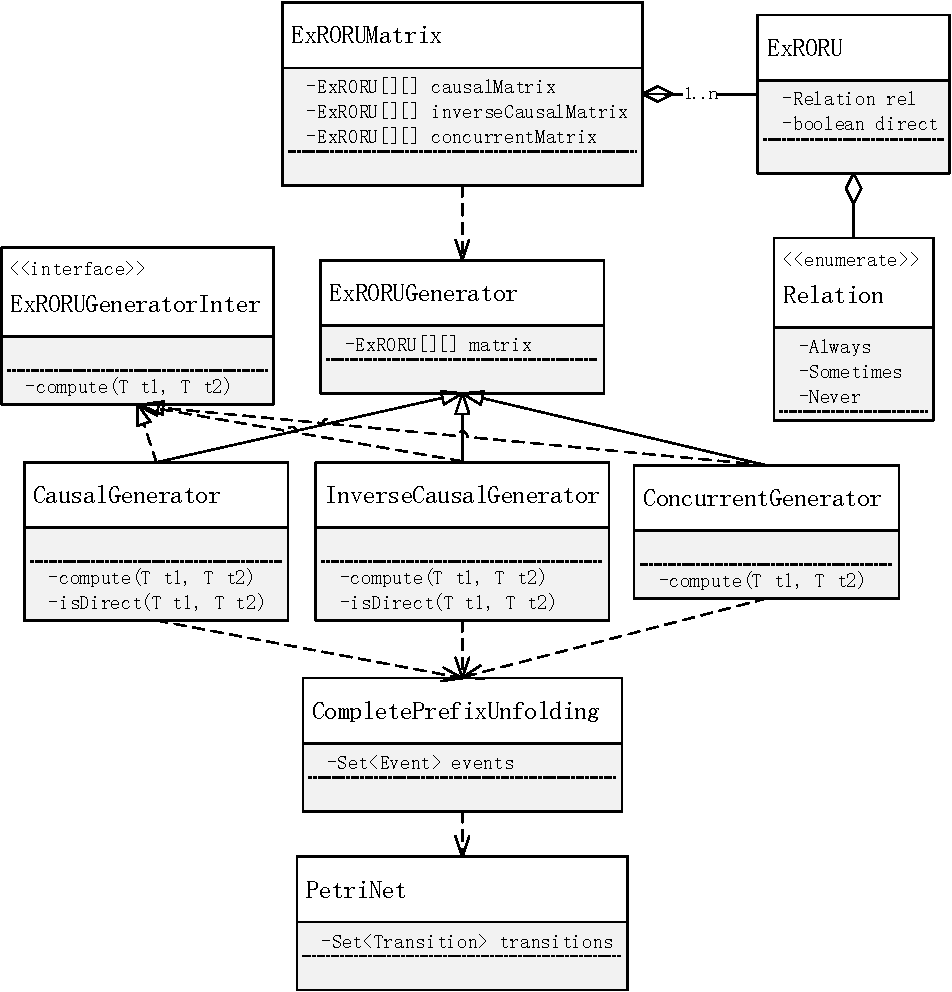
\includegraphics[width=0.9\textwidth]{class_diagram}
  \caption{ExRORU算法的实现类图}
  \label{fig:class_diagram}
\end{figure}

ExRORUMatrix是算法主类,主要功能是读入Petri网文件,并调用下层类抽取该Petri网的ExRORU矩阵。该类首先调用jbpt项目中的CPU计算方法构造给定Petri网对应的CPU,其后基于CPU抽取事件间ExRORU关系并依据前文算法折叠得到变迁间ExRORU关系。其中关键成员变量包括三个矩阵,分别对应变迁间的因果关系、逆因果关系和并行关系,每种关系都由ExRORU类记录。ExRORU类中包含标识不确定性的枚举型变量Relation和标记直接因果关系的布尔值变量(仅用于因果关系和逆因果关系)。

PetriNet类和CompletePrefixUnfolding类是jbpt项目中的原有类,分别存储Petri网和对应的完全前缀展开。在CPU的构造过程中,变迁与事件之间的对应关系也被记录下来用于后期的折叠过程。

ExRORUGenerator是抽取变迁间ExRORU关系的主类,其调用了三个不同的类分别抽取因果关系、逆因果关系和并行关系。这三个不同的类统一实现了ExRORUGeneratorInter接口,提供了compute(T t1, T t2)方法用于计算两个给定变迁之间的ExRORU关系,此外用于抽取因果关系和逆因果关系的CausalGenerator和InverseCausalGenerator还额外提供了isDirect(T t1, T t2)方法用于判定两个变迁是否满足定义\ref{def:exroru_event_causal_direct}中的直接和间接因果关系。三个类使用第\ref{cha:exroru}章介绍的算法首先基于CPU计算事件间的ExRORU关系然后将其折叠得到变迁间的ExRORU关系。

\section{实验设计与分析}\label{sec:experiment}
本节介绍ExRORU的实验设计与分析,主要包括有效性实验(将ExRORU与其他算法比较区分过程模型的能力)、性能实验(使用实际模型数据集衡量ExRORU算法的效率)和扩展性实验(衡量ExRORU处理含多并发结构过程模型的能力)等。本文实验均在一台安装了64位Windows 10教育版的台式机上完成,台式机的CPU和内存设备分别为Intel(R) Core(TM) i7-2600 CPU@3.40GHz和16.0G DDR3@1600MHz。

\subsection{有效性实验}\label{subsec:effectiveness}
本小节主要展示ExRORU算法强大的刻画过程模型行为语义的能力,并通过在多个模型实例中与第\ref{cha:related_work}章中介绍的算法对比,以说明其区分含有不同行为语义的过程模型的能力。

{\heiti 非自由选择结构\qquad}过程模型的任务之间存在间接依赖关系\cite{van2004workflow,van2003workflow,de2003workflow,van2004process},在WF-net上造成了非自由选择结构的存在(即选择关系与同步关系混合的情况)。图\ref{fig:nfc_example_1}中的模型是一个典型的含有非自由选择结构的模型,其中变迁$D$和变迁$E$之间存在非自由选择情形,即他们的执行并不由自身所决定,而是由之前被执行的变迁$A$和变迁$B$决定。具体分析,当在该WF-net的源库所$P_{0}$中放置一个托肯时,变迁$A$和变迁$B$同时被使能,若此时选择触发变迁$A$,则会在库所$_{1}$和库所$P_{2}$中各产生一个托肯;此时只有变迁$C$被使能,其被触发之后会消耗库所$P_{1}$的托肯,同时在库所$P_{4}$中产生一个托肯;库所$P_{2}$和库所$P_{4}$各有一个托肯时,显然只有变迁$D$被使能。另一方面,若一开始选择触发变迁$B$,同理可知在变迁$C$被触发之后只有变迁$E$被使能。因此,该模型的变迁执行序列只有$\langle A,C,D\rangle$和$\langle B,C,E\rangle$两条。

与之相对的是图\ref{fig:nfc_example_2}中不含有非自由选择结构的模型。与图\ref{fig:nfc_example_1}中的模型相比,该模型少了两个库所和四条边,其中变迁$D$和变迁$E$不存在非自由选择情形,即他们的执行由自身竞争库所$P_{2}$中的托肯所决定。因此,该模型的变迁执行序列有$\langle A,C,D\rangle$、$\langle A,C,E\rangle$、$\langle B,C,D\rangle$和$\langle B,C,E\rangle$四条。

以TAR算法为例,两个模型的TAR集合都是$\{\langle A,C\rangle,\langle C,D\rangle,\langle B,C\rangle,\langle C,E\rangle\}$,显然TAR算法未考虑非自由选择结构蕴含的任务间接依赖关系,所以无法区分这一组模型的行为。本文改进的基础RORU算法是通过任务间关系传递性来抽取因果关系的,然而在图\ref{fig:nfc_example_1}的模型中,变迁$A$与$C$之间的因果关系和变迁$C$与$E$之间的因果关系并不满足传递性,故RORU算法在处理该模型时会出错。

实际上,图\ref{fig:nfc_example_1}的模型只有两个过程流,分别表示为$[A\{C\}D]$和$[B\{C\}E]$(虽然在变迁$A$和变迁$B$后都有并行结构,但是均只有一个分支含有变迁$C$,另一个分支是无变迁分支)。因此,在该模型中,变迁$A$和变迁$D$满足“间接总是因果关系”,即$A\overset{\text{\tiny{IA}}}{\rightarrow}D$;变迁$B$和变迁$E$也满足“间接总是因果关系”,即$B\overset{\text{\tiny{IA}}}{\rightarrow}E$。另一方面,图\ref{fig:nfc_example_2}的模型有4个过程流,分别表示为$[ACD]$、$[ACE]$、$[BCD]$和$[BCE]$,因此在该模型中变迁$A$和变迁$D$满足“间接有时因果关系”,即$A\overset{\text{\tiny{IS}}}{\rightarrow}D$;变迁$B$和变迁$E$也满足“间接有时因果关系”,即$B\overset{\text{\tiny{IS}}}{\rightarrow}E$。两个模型的ExRORU关系矩阵如表\ref{tab:nfc_example_matrix}所示,两个模型的行为差异主要体现在变迁$A$与变迁$D$、变迁$E$之间的因果关系和逆因果关系以及变迁$B$与变迁$D$、变迁$E$之间的因果关系和逆因果关系上。因此,ExRORU算法可以检测该组模型之间的差异。

\begin{table}[htbp]
  \centering
  \setlength\tabcolsep{4pt}
  \caption{图\ref{fig:nfc_example}中两个模型的ExRORU矩阵}
  \label{tab:nfc_example_matrix}
  \vspace{6pt}
  \begin{subtable}{1\textwidth}
    \centering
    \caption{图\ref{fig:nfc_example_1}中模型的ExRORU矩阵}
    \label{tab:nfc_example_1_matrix}
    \begin{minipage}[b]{0.3\textwidth}
      \centering
      \begin{tabular}{|c|c|c|c|c|c|} \hline
        $\rightarrow$ & $A$ & $B$ & $C$ & $D$ & $E$\\ \hline
        $A$ & $\overset{\text{\tiny{N}}}{\rightarrow}$ & $\overset{\text{\tiny{N}}}{\rightarrow}$ & $\overset{\text{\tiny{DA}}}{\rightarrow}$ & \cellcolor{lightgray}$\overset{\text{\tiny{DA}}}{\rightarrow}$ & \cellcolor{lightgray}$\overset{\text{\tiny{N}}}{\rightarrow}$\\ \hline
        $B$ & $\overset{\text{\tiny{N}}}{\rightarrow}$ & $\overset{\text{\tiny{N}}}{\rightarrow}$ & $\overset{\text{\tiny{DA}}}{\rightarrow}$ & \cellcolor{lightgray}$\overset{\text{\tiny{N}}}{\rightarrow}$ & \cellcolor{lightgray}$\overset{\text{\tiny{DA}}}{\rightarrow}$\\ \hline
        $C$ & $\overset{\text{\tiny{N}}}{\rightarrow}$ & $\overset{\text{\tiny{N}}}{\rightarrow}$ & $\overset{\text{\tiny{N}}}{\rightarrow}$ & $\overset{\text{\tiny{DS}}}{\rightarrow}$ & $\overset{\text{\tiny{DS}}}{\rightarrow}$\\ \hline
        $D$ & $\overset{\text{\tiny{N}}}{\rightarrow}$ & $\overset{\text{\tiny{N}}}{\rightarrow}$ & $\overset{\text{\tiny{N}}}{\rightarrow}$ & $\overset{\text{\tiny{N}}}{\rightarrow}$ & $\overset{\text{\tiny{N}}}{\rightarrow}$\\ \hline
        $E$ & $\overset{\text{\tiny{N}}}{\rightarrow}$ & $\overset{\text{\tiny{N}}}{\rightarrow}$ & $\overset{\text{\tiny{N}}}{\rightarrow}$ & $\overset{\text{\tiny{N}}}{\rightarrow}$ & $\overset{\text{\tiny{N}}}{\rightarrow}$\\ \hline
      \end{tabular}
    \end{minipage}
    \begin{minipage}[b]{0.3\textwidth}
      \centering
      \begin{tabular}{|c|c|c|c|c|c|} \hline
        $\leftarrow$ & $A$ & $B$ & $C$ & $D$ & $E$\\ \hline
        $A$ & $\overset{\text{\tiny{N}}}{\leftarrow}$ & $\overset{\text{\tiny{N}}}{\leftarrow}$ & $\overset{\text{\tiny{N}}}{\leftarrow}$ & $\overset{\text{\tiny{N}}}{\leftarrow}$ & $\overset{\text{\tiny{N}}}{\leftarrow}$\\ \hline
        $B$ & $\overset{\text{\tiny{N}}}{\leftarrow}$ & $\overset{\text{\tiny{N}}}{\leftarrow}$ & $\overset{\text{\tiny{N}}}{\leftarrow}$ & $\overset{\text{\tiny{N}}}{\leftarrow}$ & $\overset{\text{\tiny{N}}}{\leftarrow}$\\ \hline
        $C$ & $\overset{\text{\tiny{DS}}}{\leftarrow}$ & $\overset{\text{\tiny{DS}}}{\leftarrow}$ & $\overset{\text{\tiny{N}}}{\leftarrow}$ & $\overset{\text{\tiny{N}}}{\leftarrow}$ & $\overset{\text{\tiny{N}}}{\leftarrow}$\\ \hline
        $D$ & \cellcolor{lightgray}$\overset{\text{\tiny{DA}}}{\leftarrow}$ & \cellcolor{lightgray}$\overset{\text{\tiny{N}}}{\leftarrow}$ & $\overset{\text{\tiny{DA}}}{\leftarrow}$ & $\overset{\text{\tiny{N}}}{\leftarrow}$ & $\overset{\text{\tiny{N}}}{\leftarrow}$\\ \hline
        $E$ & \cellcolor{lightgray}$\overset{\text{\tiny{N}}}{\leftarrow}$ & \cellcolor{lightgray}$\overset{\text{\tiny{DA}}}{\leftarrow}$ & $\overset{\text{\tiny{DA}}}{\leftarrow}$ & $\overset{\text{\tiny{N}}}{\leftarrow}$ & $\overset{\text{\tiny{N}}}{\leftarrow}$\\ \hline
      \end{tabular}
    \end{minipage}
    \begin{minipage}[b]{0.3\textwidth}
      \centering
      \begin{tabular}{|c|c|c|c|c|c|} \hline
        $\parallel$ & $A$ & $B$ & $C$ & $D$ & $E$\\ \hline
        $A$ & $\nparallel$ & $\nparallel$ & $\nparallel$ & $\nparallel$ & $\nparallel$\\ \hline
        $B$ & $\nparallel$ & $\nparallel$ & $\nparallel$ & $\nparallel$ & $\nparallel$\\ \hline
        $C$ & $\nparallel$ & $\nparallel$ & $\nparallel$ & $\nparallel$ & $\nparallel$\\ \hline
        $D$ & $\nparallel$ & $\nparallel$ & $\nparallel$ & $\nparallel$ & $\nparallel$\\ \hline
        $E$ & $\nparallel$ & $\nparallel$ & $\nparallel$ & $\nparallel$ & $\nparallel$\\ \hline
      \end{tabular}
    \end{minipage}
  \end{subtable}

  \begin{subtable}{1\textwidth}
    \vspace{1em}
    \centering
    \caption{图\ref{fig:nfc_example_2}中模型的ExRORU矩阵}
    \label{tab:nfc_example_2_matrix}
    \begin{minipage}[b]{0.3\textwidth}
      \centering
      \begin{tabular}{|c|c|c|c|c|c|} \hline
        $\rightarrow$ & $A$ & $B$ & $C$ & $D$ & $E$\\ \hline
        $A$ & $\overset{\text{\tiny{N}}}{\rightarrow}$ & $\overset{\text{\tiny{N}}}{\rightarrow}$ & $\overset{\text{\tiny{DA}}}{\rightarrow}$ & \cellcolor{lightgray}$\overset{\text{\tiny{DS}}}{\rightarrow}$ & \cellcolor{lightgray}$\overset{\text{\tiny{DS}}}{\rightarrow}$\\ \hline
        $B$ & $\overset{\text{\tiny{N}}}{\rightarrow}$ & $\overset{\text{\tiny{N}}}{\rightarrow}$ & $\overset{\text{\tiny{DA}}}{\rightarrow}$ & \cellcolor{lightgray}$\overset{\text{\tiny{DS}}}{\rightarrow}$ & \cellcolor{lightgray}$\overset{\text{\tiny{DS}}}{\rightarrow}$\\ \hline
        $C$ & $\overset{\text{\tiny{N}}}{\rightarrow}$ & $\overset{\text{\tiny{N}}}{\rightarrow}$ & $\overset{\text{\tiny{N}}}{\rightarrow}$ & $\overset{\text{\tiny{DS}}}{\rightarrow}$ & $\overset{\text{\tiny{DS}}}{\rightarrow}$\\ \hline
        $D$ & $\overset{\text{\tiny{N}}}{\rightarrow}$ & $\overset{\text{\tiny{N}}}{\rightarrow}$ & $\overset{\text{\tiny{N}}}{\rightarrow}$ & $\overset{\text{\tiny{N}}}{\rightarrow}$ & $\overset{\text{\tiny{N}}}{\rightarrow}$\\ \hline
        $E$ & $\overset{\text{\tiny{N}}}{\rightarrow}$ & $\overset{\text{\tiny{N}}}{\rightarrow}$ & $\overset{\text{\tiny{N}}}{\rightarrow}$ & $\overset{\text{\tiny{N}}}{\rightarrow}$ & $\overset{\text{\tiny{N}}}{\rightarrow}$\\ \hline
      \end{tabular}
    \end{minipage}
    \begin{minipage}[b]{0.3\textwidth}
      \centering
      \begin{tabular}{|c|c|c|c|c|c|} \hline
        $\leftarrow$ & $A$ & $B$ & $C$ & $D$ & $E$\\ \hline
        $A$ & $\overset{\text{\tiny{N}}}{\leftarrow}$ & $\overset{\text{\tiny{N}}}{\leftarrow}$ & $\overset{\text{\tiny{N}}}{\leftarrow}$ & $\overset{\text{\tiny{N}}}{\leftarrow}$ & $\overset{\text{\tiny{N}}}{\leftarrow}$\\ \hline
        $B$ & $\overset{\text{\tiny{N}}}{\leftarrow}$ & $\overset{\text{\tiny{N}}}{\leftarrow}$ & $\overset{\text{\tiny{N}}}{\leftarrow}$ & $\overset{\text{\tiny{N}}}{\leftarrow}$ & $\overset{\text{\tiny{N}}}{\leftarrow}$\\ \hline
        $C$ & $\overset{\text{\tiny{DS}}}{\leftarrow}$ & $\overset{\text{\tiny{DS}}}{\leftarrow}$ & $\overset{\text{\tiny{N}}}{\leftarrow}$ & $\overset{\text{\tiny{N}}}{\leftarrow}$ & $\overset{\text{\tiny{N}}}{\leftarrow}$\\ \hline
        $D$ & \cellcolor{lightgray}$\overset{\text{\tiny{DS}}}{\leftarrow}$ & \cellcolor{lightgray}$\overset{\text{\tiny{DS}}}{\leftarrow}$ & $\overset{\text{\tiny{DA}}}{\leftarrow}$ & $\overset{\text{\tiny{N}}}{\leftarrow}$ & $\overset{\text{\tiny{N}}}{\leftarrow}$\\ \hline
        $E$ & \cellcolor{lightgray}\cellcolor{lightgray}$\overset{\text{\tiny{DS}}}{\leftarrow}$ & \cellcolor{lightgray}$\overset{\text{\tiny{DS}}}{\leftarrow}$ & $\overset{\text{\tiny{DA}}}{\leftarrow}$ & $\overset{\text{\tiny{N}}}{\leftarrow}$ & $\overset{\text{\tiny{N}}}{\leftarrow}$\\ \hline
      \end{tabular}
    \end{minipage}
    \begin{minipage}[b]{0.3\textwidth}
      \centering
      \begin{tabular}{|c|c|c|c|c|c|} \hline
        $\parallel$ & $A$ & $B$ & $C$ & $D$ & $E$\\ \hline
        $A$ & $\nparallel$ & $\nparallel$ & $\nparallel$ & $\nparallel$ & $\nparallel$\\ \hline
        $B$ & $\nparallel$ & $\nparallel$ & $\nparallel$ & $\nparallel$ & $\nparallel$\\ \hline
        $C$ & $\nparallel$ & $\nparallel$ & $\nparallel$ & $\nparallel$ & $\nparallel$\\ \hline
        $D$ & $\nparallel$ & $\nparallel$ & $\nparallel$ & $\nparallel$ & $\nparallel$\\ \hline
        $E$ & $\nparallel$ & $\nparallel$ & $\nparallel$ & $\nparallel$ & $\nparallel$\\ \hline
      \end{tabular}
    \end{minipage}
  \end{subtable}
\end{table}

{\heiti 多关系\qquad}如本文算法所述,过程模型中的两个变迁$X$和$Y$之间可能存在多种类型的关系。如图\ref{fig:multi_relation}所示,图\subref{fig:multi_relation_petri}是含有多关系变迁对的WF-net示例,图\subref{fig:multi_relation_cpu}是其对应的CPU,其中变迁$A$和变迁$D$可以同时满足因果关系和并行关系。具体分析,当在该WF-net的源库所$P_{0}$中放置一个托肯时,变迁$I$被使能,当其被触发后,会在库所$P_{1}$和库所$P_{2}$中各产生一个托肯;接下来触发变迁$A$,则此时库所$P_{2}$和库所$P_{3}$中各有一个托肯,变迁$B$、变迁$C$和变迁$E$同时被使能;在这种情况下,若选择触发变迁$E$则会同时消耗两个托肯,并在库所$P_{4}$和库所$P_{5}$中各产生一个托肯,变迁$B$和变迁$C$都被跳过,然而若触发变迁$B$或者变迁$C$,则会夺走变迁$E$输入库所中的托肯使其不能被触发。

从CPU中可知该模型共有两个过程流,分别表示为$[I\{AC,BD\}O]$和$[I\{A\}E\{D\}O]$,由ExRORU算法得到变迁$A$和变迁$D$满足“间接有时因果关系”,即$A\overset{\text{\tiny{IS}}}{\rightarrow}D$;同时它们满足“有时并行关系”,即$A\Uparrow D$。

\begin{figure}[htbp]
  \centering
  \begin{subfigure}{1\textwidth}
    \centering
    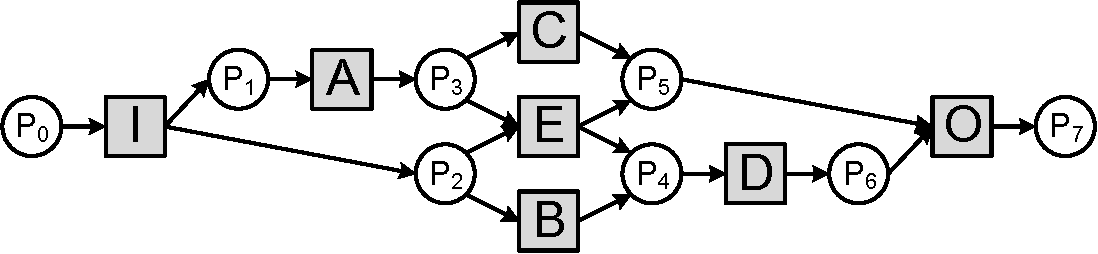
\includegraphics[width=0.9\textwidth]{multi_relation_petri}
    \caption{含有多关系变迁对的WF-net}
    \label{fig:multi_relation_petri}
  \end{subfigure}
  \begin{subfigure}{1\textwidth}
    \vspace{1em}
    \centering
    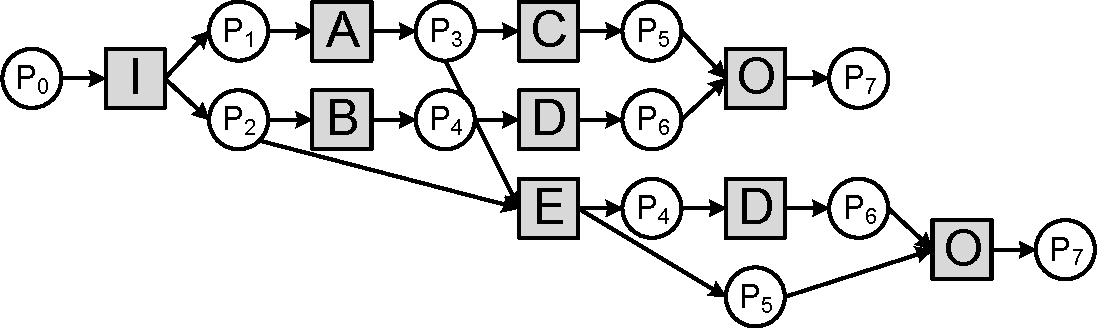
\includegraphics[width=0.9\textwidth]{multi_relation_cpu}
    \caption{图\subref{fig:multi_relation_petri}中WF-net对应的CPU}
    \label{fig:multi_relation_cpu}
  \end{subfigure}
  \vspace{6pt}
  \caption{含有多关系变迁对的模型示例}
  \label{fig:multi_relation}
\end{figure}

绝大多数算法如BP、TAR等都不能识别变迁对之间多关系的存在,因为它们将每对变迁之间的关系定义为单独一种,因此这些算法也无法准确地刻画过程模型的行为语义从而不能有效地区分含有多关系变迁对的模型。虽然RORU算法允许一对变迁之间存在多种关系,但是它并没有对一个变迁在CPU中对应多个事件的情况作处理。根据RORU的计算方法,CPU中的每个事件都被当作独立事件参与事件间RORU关系的计算,RORU并没有提及如何将多个对应事件与其他事件的关系折叠回原始变迁对之间的RORU关系。例如,在图\ref{fig:multi_relation}的模型中,RORU无法确定变迁$D$(变迁$D$在图\ref{fig:multi_relation_cpu}的CPU中有两个对应事件,变迁$O$也一样)和其他变迁之间的关系。

{\heiti 不可见变迁\qquad}不可见变迁是一类不会在过程模型执行轨迹中出现的变迁,以下情形都会导致不可见变迁的出现:
\begin{itemize}
  \item[-] 过程模型中存在只含有路由功能的无意义任务;
  \item[-] 在实际执行轨迹中会出现任务被漏记等缺失情况;
  \item[-] 过程模型中允许跳过或重做当前任务、跳回到之前某个任务的情形,但该类执行逻辑并未在过程模型的控制逻辑中表达出来。
\end{itemize}
不可见变迁不含有意义的标签,它不会在变迁执行序列中显式出现。本文使用带斜线的阴影方框表示不可见变迁。根据不可见变迁的功能,图\ref{fig:invisible_transition_types}将其分为四类。图\ref{fig:invisible_transition_skip}中的模型含有SKIP类型的不可见变迁,该类不可见变迁被用于跳过某些任务(该例中跳过了变迁$B$);图\ref{fig:invisible_transition_redo}中的模型含有REDO类型的不可见变迁,该类不可见变迁被用于重复执行某些任务(该例中重复执行变迁$B$);图\ref{fig:invisible_transition_side}中的模型含有SIDE类型的不可见变迁,该类不可见变迁与源库所或者汇库所直接相连;图\ref{fig:invisible_transition_switch}中的模型含有SWITCH类型的不可见变迁,该类不可见变迁被用于在不同分支之间切换执行权(该例中从含有变迁$A$和$C$的分支切换到含有变迁$B$和$D$的分支)。

\begin{figure}[htbp]
  \centering
  \begin{subfigure}[b]{0.48\textwidth}
    \centering
    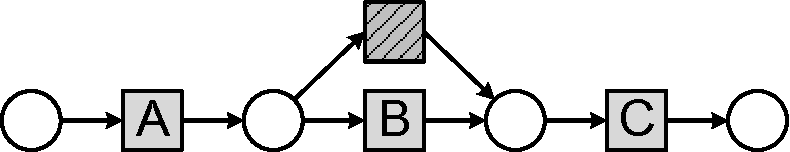
\includegraphics[width=0.98\textwidth]{invisible_transition_skip}
    \caption{SKIP类型的不可见变迁}
    \label{fig:invisible_transition_skip}
  \end{subfigure}
  \begin{subfigure}[b]{0.48\textwidth}
    \centering
    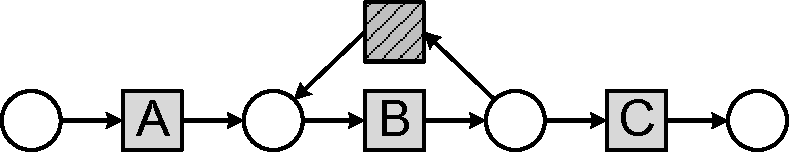
\includegraphics[width=0.98\textwidth]{invisible_transition_redo}
    \caption{REDO类型的不可见变迁}
    \label{fig:invisible_transition_redo}
  \end{subfigure}
  \begin{subfigure}[b]{0.48\textwidth}
    \vspace{1em}
    \centering
    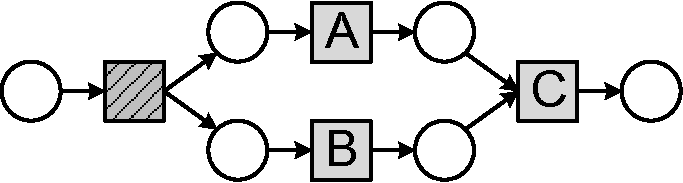
\includegraphics[width=0.98\textwidth]{invisible_transition_side}
    \caption{SIDE类型的不可见变迁}
    \label{fig:invisible_transition_side}
  \end{subfigure}
  \begin{subfigure}[b]{0.48\textwidth}
    \vspace{1em}
    \centering
    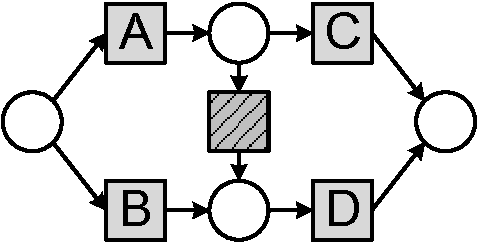
\includegraphics[width=0.7\textwidth]{invisible_transition_switch}
    \caption{SWITCH类型的不可见变迁}
    \label{fig:invisible_transition_switch}
  \end{subfigure}
  \vspace{6pt}
  \caption{四种类型的不可见变迁}
  \label{fig:invisible_transition_types}
\end{figure}

如前文所述,不可见变迁的存在能够改变过程模型的行为。图\ref{fig:sda_example}是一对含有不可见变迁的模型,两者唯一的区别在于变迁$I$和变迁$O$的关系。具体分析,在图\ref{fig:sda_example_1}的WF-net中的源库所$P_{0}$中放置一个托肯时,变迁$I$被使能,当其被触发后,会在库所$P_{1}$和库所$P_{2}$中各产生一个托肯,此时变迁$A$和变迁$B$均被使能,且满足并发执行关系;若此时将变迁$A$和变迁$B$都触发,则会在库所$P_{3}$和库所$P_{4}$中各产生一个托肯,使得中间的不可见变迁被使能;若此时只触发变迁$A$,则库所$P_{2}$和库所$P_{3}$中各有一个托肯,使得上方的不可见变迁被使能;若此时只触发变迁$B$,则库所$P_{1}$和库所$P_{4}$中各有一个托肯,使得下方的不可见变迁被使能。无论上述三种情况的哪一种发生,触发不可见变迁之后都会在库所$P_{5}$中产生一个托肯,从而使得变迁$O$被使能;当变迁$O$被触发后,过程执行完毕。该模型的变迁发生序列有四条,分别是$\langle I,A,B,O\rangle$、$\langle I,B,A,O\rangle$、$\langle I,A,O\rangle$和$\langle I,B,O\rangle$
。

与之相对应的是图\ref{fig:sda_example_2}中的WF-net,该模型中的变迁$A$和变迁$B$可以都被跳过而不被触发。当在源库所$P_{0}$中放置一个托肯时,变迁$I$被使能,当其被触发后,会在库所$P_{1}$和库所$P_{2}$中各产生一个托肯,此时变迁$A$和变迁$B$均被使能,上方和下方的两个不可见变迁也被使能了,且分别和变迁$A$、变迁$B$满足竞争关系;此时可以在上方的不可见变迁和变迁$A$中、下方的不可见变迁和变迁$B$中各选择一个触发,且触发过程满足并行关系。无论选择哪两个变迁触发,都会在库所$P_{3}$和库所$P_{4}$中各产生一个托肯,从而使得变迁$O$被使能;当变迁$O$被触发后,过程执行完毕。该模型的变迁发生序列有五条,分别是$\langle I,A,B,O\rangle$、$\langle I,B,A,O\rangle$、$\langle I,A,O\rangle$、$\langle I,B,O\rangle$和$\langle I,O\rangle$。

两个模型的行为差异在于后者比前者多了一条变迁发生序列,即变迁$I$和变迁$O$可以紧邻发生。诸如CBP、4C和RORU等以任务间关系为基础的过程模型行为语义刻画方法都没有考虑任务间紧邻关系,所以无法区分这组模型的行为语义。实际上,图\ref{fig:sda_example_1}的模型中的变迁$I$和变迁$O$满足“间接总是因果关系”,即$I\overset{\text{\tiny{IA}}}{\rightarrow}O$,而图\ref{fig:sda_example_2}的模型中的变迁$I$和变迁$O$满足“直接总是因果关系”,即$I\overset{\text{\tiny{DA}}}{\rightarrow}O$。两个模型的ExRORU关系矩阵如表\ref{tab:sda_example_matrix}所示,两个模型的行为差异主要体现在变迁$I$和变迁$O$之间的因果关系和逆因果关系上。因此,ExRORU算法可以检测该组模型之间的差异。

\begin{table}[htbp]
  \centering
  % \setlength\tabcolsep{4pt}
  \caption{图\ref{fig:sda_example}中两个模型的ExRORU矩阵}
  \label{tab:sda_example_matrix}
  \begin{subtable}{1\textwidth}
    \centering
    \caption{图\ref{fig:sda_example_1}中模型的ExRORU矩阵}
    \label{tab:sda_example_1_matrix}
    \begin{minipage}[b]{0.3\textwidth}
      \centering
      \begin{tabular}{|c|c|c|c|c|} \hline
        $\rightarrow$ & $I$ & $A$ & $B$ & $O$\\ \hline
        $I$ & $\overset{\text{\tiny{N}}}{\rightarrow}$ & $\overset{\text{\tiny{DS}}}{\rightarrow}$ & $\overset{\text{\tiny{DS}}}{\rightarrow}$ & \cellcolor{lightgray}$\overset{\text{\tiny{IA}}}{\rightarrow}$\\ \hline
        $A$ & $\overset{\text{\tiny{N}}}{\rightarrow}$ & $\overset{\text{\tiny{N}}}{\rightarrow}$ & $\overset{\text{\tiny{N}}}{\rightarrow}$ & $\overset{\text{\tiny{DA}}}{\rightarrow}$\\ \hline
        $B$ & $\overset{\text{\tiny{N}}}{\rightarrow}$ & $\overset{\text{\tiny{N}}}{\rightarrow}$ & $\overset{\text{\tiny{N}}}{\rightarrow}$ & $\overset{\text{\tiny{DA}}}{\rightarrow}$\\ \hline
        $O$ & $\overset{\text{\tiny{N}}}{\rightarrow}$ & $\overset{\text{\tiny{N}}}{\rightarrow}$ & $\overset{\text{\tiny{N}}}{\rightarrow}$ & $\overset{\text{\tiny{N}}}{\rightarrow}$\\ \hline
      \end{tabular}
    \end{minipage}
    \begin{minipage}[b]{0.3\textwidth}
      \centering
      \begin{tabular}{|c|c|c|c|c|} \hline
        $\leftarrow$ & $I$ & $A$ & $B$ & $O$\\ \hline
        $I$ & $\overset{\text{\tiny{N}}}{\leftarrow}$ & $\overset{\text{\tiny{N}}}{\leftarrow}$ & $\overset{\text{\tiny{N}}}{\leftarrow}$ & $\overset{\text{\tiny{N}}}{\leftarrow}$\\ \hline
        $A$ & $\overset{\text{\tiny{DA}}}{\leftarrow}$ & $\overset{\text{\tiny{N}}}{\leftarrow}$ & $\overset{\text{\tiny{N}}}{\leftarrow}$ & $\overset{\text{\tiny{N}}}{\leftarrow}$\\ \hline
        $B$ & $\overset{\text{\tiny{DA}}}{\leftarrow}$ & $\overset{\text{\tiny{N}}}{\leftarrow}$ & $\overset{\text{\tiny{N}}}{\leftarrow}$ & $\overset{\text{\tiny{N}}}{\leftarrow}$\\ \hline
        $O$ & \cellcolor{lightgray}$\overset{\text{\tiny{IA}}}{\leftarrow}$ & $\overset{\text{\tiny{DS}}}{\leftarrow}$ & $\overset{\text{\tiny{DS}}}{\leftarrow}$ & $\overset{\text{\tiny{N}}}{\leftarrow}$\\ \hline
      \end{tabular}
    \end{minipage}
    \begin{minipage}[b]{0.3\textwidth}
      \centering
      \begin{tabular}{|c|c|c|c|c|} \hline
        $\parallel$ & $I$ & $A$ & $B$ & $O$\\ \hline
        $I$ & $\nparallel$ & $\nparallel$ & $\nparallel$ & $\nparallel$\\ \hline
        $A$ & $\nparallel$ & $\nparallel$ & $\Uparrow$ & $\nparallel$\\ \hline
        $B$ & $\nparallel$ & $\Uparrow$ & $\nparallel$ & $\nparallel$\\ \hline
        $O$ & $\nparallel$ & $\nparallel$ & $\nparallel$ & $\nparallel$\\ \hline
      \end{tabular}
    \end{minipage}
  \end{subtable}

  \begin{subtable}{1\textwidth}
    \vspace{1em}
    \centering
    \caption{图\ref{fig:sda_example_2}中模型的ExRORU矩阵}
    \label{tab:sda_example_2_matrix}
    \begin{minipage}[b]{0.3\textwidth}
      \centering
      \begin{tabular}{|c|c|c|c|c|} \hline
        $\rightarrow$ & $I$ & $A$ & $B$ & $O$\\ \hline
        $I$ & $\overset{\text{\tiny{N}}}{\rightarrow}$ & $\overset{\text{\tiny{DS}}}{\rightarrow}$ & $\overset{\text{\tiny{DS}}}{\rightarrow}$ & \cellcolor{lightgray}$\overset{\text{\tiny{DA}}}{\rightarrow}$\\ \hline
        $A$ & $\overset{\text{\tiny{N}}}{\rightarrow}$ & $\overset{\text{\tiny{N}}}{\rightarrow}$ & $\overset{\text{\tiny{N}}}{\rightarrow}$ & $\overset{\text{\tiny{DA}}}{\rightarrow}$\\ \hline
        $B$ & $\overset{\text{\tiny{N}}}{\rightarrow}$ & $\overset{\text{\tiny{N}}}{\rightarrow}$ & $\overset{\text{\tiny{N}}}{\rightarrow}$ & $\overset{\text{\tiny{DA}}}{\rightarrow}$\\ \hline
        $O$ & $\overset{\text{\tiny{N}}}{\rightarrow}$ & $\overset{\text{\tiny{N}}}{\rightarrow}$ & $\overset{\text{\tiny{N}}}{\rightarrow}$ & $\overset{\text{\tiny{N}}}{\rightarrow}$\\ \hline
      \end{tabular}
    \end{minipage}
    \begin{minipage}[b]{0.3\textwidth}
      \centering
      \begin{tabular}{|c|c|c|c|c|} \hline
        $\leftarrow$ & $I$ & $A$ & $B$ & $O$\\ \hline
        $I$ & $\overset{\text{\tiny{N}}}{\leftarrow}$ & $\overset{\text{\tiny{N}}}{\leftarrow}$ & $\overset{\text{\tiny{N}}}{\leftarrow}$ & $\overset{\text{\tiny{N}}}{\leftarrow}$\\ \hline
        $A$ & $\overset{\text{\tiny{DA}}}{\leftarrow}$ & $\overset{\text{\tiny{N}}}{\leftarrow}$ & $\overset{\text{\tiny{N}}}{\leftarrow}$ & $\overset{\text{\tiny{N}}}{\leftarrow}$\\ \hline
        $B$ & $\overset{\text{\tiny{DA}}}{\leftarrow}$ & $\overset{\text{\tiny{N}}}{\leftarrow}$ & $\overset{\text{\tiny{N}}}{\leftarrow}$ & $\overset{\text{\tiny{N}}}{\leftarrow}$\\ \hline
        $O$ & \cellcolor{lightgray}$\overset{\text{\tiny{DA}}}{\leftarrow}$ & $\overset{\text{\tiny{DS}}}{\leftarrow}$ & $\overset{\text{\tiny{DS}}}{\leftarrow}$ & $\overset{\text{\tiny{N}}}{\leftarrow}$\\ \hline
      \end{tabular}
    \end{minipage}
    \begin{minipage}[b]{0.3\textwidth}
      \centering
      \begin{tabular}{|c|c|c|c|c|} \hline
        $\parallel$ & $I$ & $A$ & $B$ & $O$\\ \hline
        $I$ & $\nparallel$ & $\nparallel$ & $\nparallel$ & $\nparallel$\\ \hline
        $A$ & $\nparallel$ & $\nparallel$ & $\Uparrow$ & $\nparallel$\\ \hline
        $B$ & $\nparallel$ & $\Uparrow$ & $\nparallel$ & $\nparallel$\\ \hline
        $O$ & $\nparallel$ & $\nparallel$ & $\nparallel$ & $\nparallel$\\ \hline
      \end{tabular}
    \end{minipage}
  \end{subtable}
\end{table}

图\ref{fig:invisible_transition_examples}给出了更多的含有不可见变迁的过程模型对。本文的ExRORU算法可以检测到其中各组模型之间的行为差异。在图\ref{fig:invisible_transition_a}的上方模型中,变迁$A$和变迁$B$满足“直接总是因果关系”,即$A\overset{\text{\tiny{DA}}}{\rightarrow}B$,变迁$A$和变迁$C$满足“间接总是因果关系”,即$A\overset{\text{\tiny{IA}}}{\rightarrow}C$;而在下方模型中,变迁$A$和变迁$B$满足“直接有时因果关系”,即$A\overset{\text{\tiny{DS}}}{\rightarrow}B$,变迁$A$和变迁$C$满足“直接总是因果关系”,即$A\overset{\text{\tiny{DA}}}{\rightarrow}C$。

在图\ref{fig:invisible_transition_b}和图\ref{fig:invisible_transition_c}的上方模型中,变迁$B$和变迁$C$都满足“有时并行关系”,即$B\Uparrow C$,而在两幅图的下方模型中,变迁$B$和变迁$C$都满足“总是并行关系”,即$B\Updownarrow C$。

CBP等算法不考虑任务间紧邻关系也不区分并行关系的不确定性,所以无法区分图中的三组模型。TAR算法虽然考虑了任务间紧邻关系,但是对于并行关系刻画的不准确导致了它无法区分图\ref{fig:invisible_transition_b}和图\ref{fig:invisible_transition_c}中的两对模型。类似的,RORU算法无法处理这些含有不可见变迁的模型,且它不能计算图\ref{fig:invisible_transition_c}中这样带环的模型。

\begin{figure}[htbp]
  \centering
  \begin{subfigure}{1\textwidth}
    \centering
    \begin{minipage}[b]{0.45\textwidth}
      \centering
      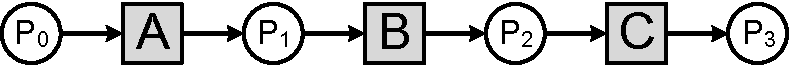
\includegraphics[width=1\textwidth]{invisible_transition_a_1}
    \end{minipage}
    \hspace{1em}
    \begin{minipage}[b]{0.45\textwidth}
      \centering
      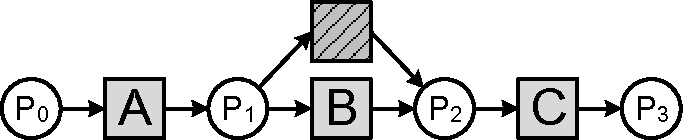
\includegraphics[width=1\textwidth]{invisible_transition_a_2}
    \end{minipage}
    \caption{}
    \label{fig:invisible_transition_a}
  \end{subfigure}
  \begin{subfigure}{1\textwidth}
    \vspace{1em}
    \centering
    \begin{minipage}[]{0.45\textwidth}
      \centering
      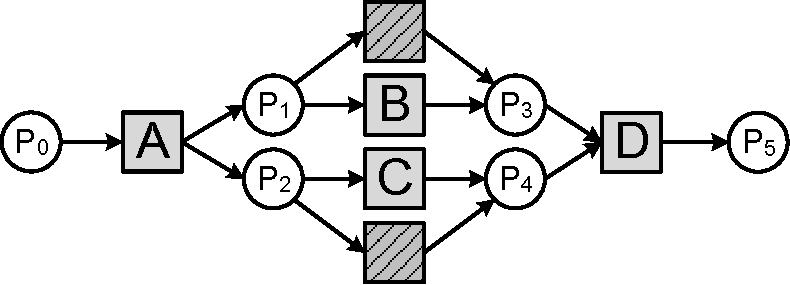
\includegraphics[width=1\textwidth]{invisible_transition_b_1}
    \end{minipage}
    \hspace{1em}
    \begin{minipage}[]{0.45\textwidth}
      \centering
      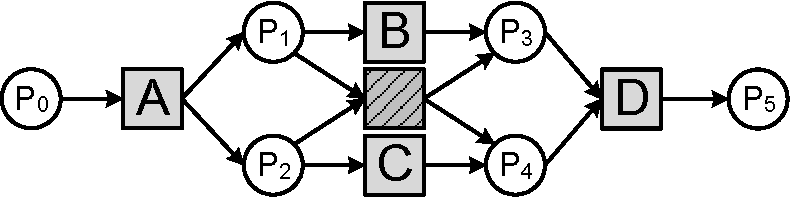
\includegraphics[width=1\textwidth]{invisible_transition_b_2}
    \end{minipage}
    \caption{}
    \label{fig:invisible_transition_b}
  \end{subfigure}
  \begin{subfigure}{1\textwidth}
    \vspace{1em}
    \centering
    \begin{minipage}[]{0.45\textwidth}
      \centering
      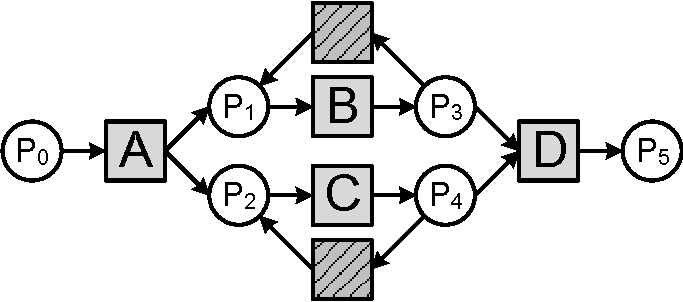
\includegraphics[width=1\textwidth]{invisible_transition_c_1}
    \end{minipage}
    \hspace{1em}
    \begin{minipage}[]{0.45\textwidth}
      \centering
      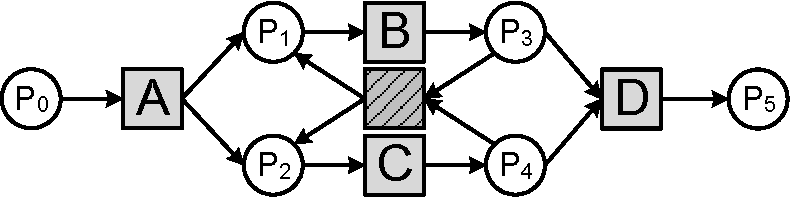
\includegraphics[width=1\textwidth]{invisible_transition_c_2}
    \end{minipage}
    \caption{}
    \label{fig:invisible_transition_c}
  \end{subfigure}
  \vspace{6pt}
  \caption{含有不可见变迁的WF-net示例}
  \label{fig:invisible_transition_examples}
\end{figure}

\subsection{性能实验}\label{subsec:efficiency}
本文使用企业中的实际模型作为数据集测试ExRORU算法的性能,表\ref{tab:efficiency_dataset}给出了这些数据集的基本结构特征。将ExRORU算法分别应用到这些数据集上,表格的最后一列是ExRORU算法在抽取每个过程模型行为特征的平均耗时。
\begin{itemize}
  \item[-] SAP数据集来自于世界著名ERP(Enterprise Resource Planning,企业资源计划)服务提供商SAP公司。原始的SAP数据集中包含604个SAP参考模型,本文删除了其中不满足定义\ref{def:sound}所述合理性的模型。最终筛选后的数据集包含389个模型。
  \item[-] DG数据集来自于东方锅炉股份有限公司,包含94个模型。东方锅炉股份有限公司是中国一流的火力发电设备、核电站设备、电机辅机、环保设备、化工容器、煤气化设备等的制造商和服务提供商。
  \item[-] TC数据集来自于唐山轨道客车有限责任公司,包含89个模型。始建于1881年的唐山轨道客车有限责任公司是中国第一家轨道装备制造企业。
\end{itemize}

从表\ref{tab:efficiency_dataset}中可以看出,ExRORU算法在来自企业的实际过程模型数据集中表现良好,能够在几毫秒至几十毫秒的时间范围内抽取过程模型的ExRORU关系矩阵,该耗时规模在实际应用中完全满足业务需求。

\begin{table}[htbp]
  \centering
  \caption{各企业实际业务过程模型集的结构特征及ExRORU算法的性能表现}
  \label{tab:efficiency_dataset}
  \begin{tabular}{lrrrrrrrr}
    \toprule[1.5pt]
    数据集 & 规模 & \tabincell{r}{平均\\变迁数} & \tabincell{r}{平均\\库所数} & \tabincell{r}{平均\\边数} & \tabincell{r}{最大\\变迁数} & \tabincell{r}{最大\\库所数} & \tabincell{r}{最大\\边数} & \tabincell{r}{平均耗时\\(毫秒)}\\ \midrule[1pt]
    SAP & 389 & 4.47 & 7.51 & 11.51 & 21 & 31 & 56 & 1.43\\
    DG & 94 & 8.56 & 8.89 & 17.78 & 34 & 33 & 70 & 10.89\\
    TC & 89 & 11.47 & 10.28 & 22.93 & 28 & 29 & 58 & 15.34\\
    \bottomrule[1.5pt]
  \end{tabular}
\end{table}

\subsection{扩展性实验}\label{subsec:scalability}
诸多过程模型行为语义刻画和相似性度量算法都会面临状态爆炸问题,即含有高并发分支的模型有巨大数量的状态,从而无法被相应算法快速处理。为了测试ExRORU在含有高并发分支的模型中的性能,本文设计了两组模型用于扩展性实验。第一组模型包含11个过程模型,依次含有$5,10,15,...,55$个并发分支,每个并发分支仅含有一个可见变迁,该组模型被用于进行宽度扩展性实验;第二组模型也包含11个过程模型,不同的是,该组中的每个模型都有5个并发分支,但分支上的变迁数依次递增,11个模型的分支上分别含有$1,2,3,...,11$个可见变迁,该组模型被用于进行深度扩展性实验。使用ExRORU算法分别抽取两组过程模型的行为特征的时间消耗如图\ref{fig:scalability}所示。

\begin{figure}[htbp]
  \centering
  \begin{subfigure}{0.48\textwidth}
    \centering
    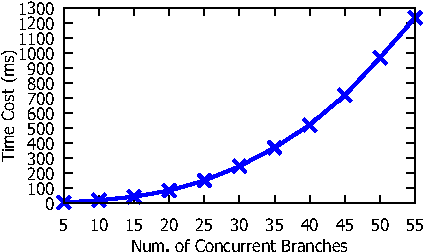
\includegraphics[width=1\textwidth]{scalability_breadth}
    \caption{宽度扩展性实验}
    \label{fig:scalability_breadth}
  \end{subfigure}
  \begin{subfigure}{0.48\textwidth}
    \centering
    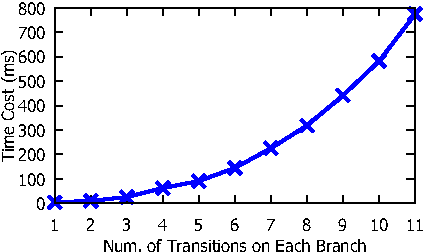
\includegraphics[width=1\textwidth]{scalability_depth}
    \caption{深度扩展性实验}
    \label{fig:scalability_depth}
  \end{subfigure}
  \vspace{6pt}
  \caption{ExRORU算法的扩展性事件结果}
  \label{fig:scalability}
\end{figure}

考虑到ExRORU算法包含任务间关系的诸多细节,扩展性实验的结果是完全可接受的。ExRORU是目前唯一可以同时处理多种复杂结构——如不可见变迁、非自由选择结构、多关系、循环结构——的算法,这显示了其杰出的性能。

\section{本章小结}
本章介绍了ExRORU算法的实现方案和实验结果。通过与其他过程模型行为语义刻画算法和相似性度量算法的比较,ExRORU拥有更为精细的刻画粒度,在含有各种复杂结构的过程模型中表现优异。同时,本文使用来自企业的实际业务过程模型数据集验证ExRORU算法的效率并使用人工创建的含高并发分支结构的过程模型数据集验证ExRORU算法的扩展性,两项实验均表明了ExRORU算法兼顾了性能和效率。
\chapter{总结与展望}\label{cha:conclusion}

\section{本文的工作总结}\label{sec:conclusion}

\section{未来工作展望}\label{sec:future_work}


%%% 其它部分
\backmatter

%% 本科生要这几个索引,研究生不要。选择性留下。
% 插图索引
% \listoffigures
% 表格索引
% \listoftables
% 公式索引
% \listofequations


%% 参考文献
% 注意:至少需要引用一篇参考文献,否则下面两行可能引起编译错误。
% 如果不需要参考文献,请将下面两行删除或注释掉。
\bibliographystyle{thuthesis}
\bibliography{ref/refs}


%% 致谢
% !TEX root = ../main.tex
% !TEX program = xelatex

% 如果使用声明扫描页,将可选参数指定为扫描后的 PDF 文件名,例如:
% \begin{ack}[scan-statement.pdf]
\begin{acknowledgement}
  % 衷心感谢导师 xxx 教授和物理系 xxx 副教授对本人的精心指导。他们的言传身教将使
  % 我终生受益。

  % 在美国麻省理工学院化学系进行九个月的合作研究期间,承蒙 xxx 教授热心指导与帮助,不
  % 胜感激。感谢 xx 实验室主任 xx 教授,以及实验室全体老师和同学们的热情帮助和支
  % 持!本课题承蒙国家自然科学基金资助,特此致谢。

  % 感谢 \thuthesis,它的存在让我的论文写作轻松自在了许多,让我的论文格式规整漂亮了
  % 许多。
  衷心感谢我的导师王建民教授在本人研究生就读期间对我的关心和指导,他不仅在学业上对我进行了规划和指导,更在人生观和价值观的塑造上让我受益匪浅。王老师讲授的工作流技术基础课程让我对工作流领域有了更深的理解和强烈的兴趣。

  衷心感谢闻立杰副教授自本科以来对本人的精心指导。闻老师带领我进入了工作流这样无限精彩的领域,他的言传身教使我在学业和生活中都有了长远的进步。

  衷心感谢所有无私指导过我的清华老师,他们的敬业、严谨让我踏入了正确的人生道路。感谢实验室和研究组中的所有同学在学习和生活中的互帮互助。

  衷心感谢我的家人和朋友,尤其是我的父母和祖父母,感谢他们对我的付出和关怀,使我成人成才,他们是我内心最坚强的精神支柱。感谢我的朋友们,他们在我前进的道路上不断地鼓励着我。
\end{acknowledgement}


%% 附录
% \begin{appendix}
% % !TEX root = ../main.tex
% !TEX program = xelatex

\chapter{ExRORU算法的唯一性证明}
\label{app:uniqueness}

\begin{theorem}[唯一性]
如果两个过程模型在其轨迹上表现出任何不同的行为,它们的ExRORU矩阵必然是不同的。
\end{theorem}

\begin{proof}
对过程模型$P$结构上的任意单步变动产生了新的过程模型$Q$,可以从三个方面证明$P$和$Q$的ExRORU矩阵是不同的:(1)改变一对变迁间的关系;(2)增加/删除一个可见变迁;(3)增加/删除一个不可见变迁。接下来从三个方面分别证明。

\textbf{(1)改变一对变迁间的关系:}如果一对关系被改变了,例如一对处于顺序结构中的变迁被改造成并行结构或者循环结构,这类基本关系的改变显然会直接反映在模型的ExRORU矩阵中,在此不加赘述。

\textbf{(2)增加/删除一个可见变迁:}一个新的可见变迁可以被添加在过程模型中,且其必然会与一个已有的变迁(更一般化地,与一个包含多个变迁和库所的子过程)同处一个顺序结构、或并行结构、或互斥结构、或循环结构,如图\ref{fig:uniqueness_2}所示。为便于展示,图中只展示了一个WF-net的部分结构,$A$和$B$是两个不同的变迁,带斜线的阴影框表示不可见变迁。矩阵中的$A$和$B$对应图中的两个变迁,$S$代表该部分结构前与之紧邻的前驱变迁,$E$代表该部分结构后与之紧邻的后继变迁。
\begin{enumerate}[(a)]
  \item 原始模型的部分结构,只含有一个可见变迁$A$,如图\ref{fig:uniqueness_2_a}。
  \item 在变迁$A$之后增加一个可见变迁$B$,与变迁$A$同处顺序结构,如图\ref{fig:uniqueness_2_b}。此时ExRORU矩阵多了有关变迁$B$的行列,显然发生了改变。
  \item 在变迁$A$之前增加一个可见变迁$B$,与变迁$A$同处顺序结构,如图\ref{fig:uniqueness_2_c}。此时ExRORU矩阵多了有关变迁$B$的行列,显然发生了改变。
  \item 增加一个可见变迁$B$,与$A$同处互斥结构,如图\ref{fig:uniqueness_2_d}。此时ExRORU矩阵多了有关变迁$B$的行列,显然发生了改变。而且,变迁$S$与变迁$A$的因果关系从“直接总是因果关系”变为“直接有时因果关系”,即$S\overset{\text{\tiny{DA}}}{\rightarrow}A\Rightarrow S\overset{\text{\tiny{DS}}}{\rightarrow}A$;变迁$E$与变迁$A$的逆因果关系从“直接总是逆因果关系”变为“直接有时逆因果关系”,即$E\overset{\text{\tiny{DA}}}{\leftarrow}A\Rightarrow E\overset{\text{\tiny{DS}}}{\leftarrow}A$。
  \item 增加一个可见变迁$B$,与$A$同处循环结构,如图\ref{fig:uniqueness_2_e}。此时ExRORU矩阵多了有关变迁$B$的行列,显然发生了改变。而且,变迁$A$与变迁$S$的逆因果关系从“直接总是逆因果关系”变为“直接有时逆因果关系”,即$A\overset{\text{\tiny{DA}}}{\leftarrow}S\Rightarrow A\overset{\text{\tiny{DS}}}{\leftarrow}S$;变迁$A$与变迁$E$的因果关系从“直接总是因果关系”变为“直接有时因果关系”,即$A\overset{\text{\tiny{DA}}}{\rightarrow}E\Rightarrow A\overset{\text{\tiny{DS}}}{\rightarrow}E$;变迁$A$与其自身的因果关系和逆因果关系从“从不因果关系”和“从不逆因果关系”变为“间接有时因果关系”和“间接有时逆因果关系”,即$A\overset{\text{\tiny{N}}}{\rightarrow}A,A\overset{\text{\tiny{N}}}{\leftarrow}A\Rightarrow A\overset{\text{\tiny{IS}}}{\rightarrow}A,A\overset{\text{\tiny{IS}}}{\leftarrow}A$。
  \item 增加一个可见变迁$B$,与$A$同处并行结构,如图\ref{fig:uniqueness_2_f}。此时ExRORU矩阵多了有关变迁$B$的行列,显然发生了改变。
\end{enumerate}
从图中可以看出,上述所有变化都会导致对应的ExRORU矩阵发生变化。因为一个新的过程模型是通过将上述单步变化连续应用在原始过程模型中产生的,归纳可知新的过程模型和原始模型拥有不同的ExRORU矩阵。类似的证明可应用于“删除一个可见变迁”中。

\textbf{(3)增加/删除一个不可见变迁:}一个新的不可见变迁也可以被添加在过程模型中,与情形(2)中的结构类似,如图\ref{fig:uniqueness_3}所示。
\begin{enumerate}[(a)]
  \item 原始模型的部分结构,只含有一个可见变迁$A$,如图\ref{fig:uniqueness_3_a}。
  \item 将变迁$A$两侧的库所合并成一个库所,如图\ref{fig:uniqueness_3_b}。变迁$S$和变迁$A$的因果关系、变迁$A$和变迁$S$的逆因果关系从“直接总是因果关系”、“直接总是逆因果关系”变为“直接有时因果关系”、“直接有时逆因果关系”,即$S\overset{\text{\tiny{DA}}}{\rightarrow}A,A\overset{\text{\tiny{DA}}}{\leftarrow}S\Rightarrow S\overset{\text{\tiny{DS}}}{\rightarrow}A,A\overset{\text{\tiny{DS}}}{\leftarrow}S$;变迁$A$和变迁$E$的因果关系、变迁$E$和变迁$A$的逆因果关系从“直接总是因果关系”、“直接总是逆因果关系”变为“直接有时因果关系”、“直接有时逆因果关系”,即$A\overset{\text{\tiny{DA}}}{\rightarrow}E,E\overset{\text{\tiny{DA}}}{\leftarrow}A\Rightarrow A\overset{\text{\tiny{DS}}}{\rightarrow}E,E\overset{\text{\tiny{DS}}}{\leftarrow}A$;变迁$A$与其自身的因果关系和逆因果关系从“从不因果关系”和“从不逆因果关系”变为“直接有时因果关系”和“直接有时逆因果关系”,即$A\overset{\text{\tiny{N}}}{\rightarrow}A,A\overset{\text{\tiny{N}}}{\leftarrow}A\Rightarrow A\overset{\text{\tiny{DS}}}{\rightarrow}A,A\overset{\text{\tiny{DS}}}{\leftarrow}A$;变迁$S$和变迁$E$的因果关系、变迁$E$与变迁$S$的逆因果关系从“间接总是因果关系”、“间接总是逆因果关系”变为“直接总是因果关系”、“直接总是逆因果关系”,即$S\overset{\text{\tiny{IA}}}{\rightarrow}E,E\overset{\text{\tiny{IA}}}{\leftarrow}S\Rightarrow S\overset{\text{\tiny{DA}}}{\rightarrow}E,E\overset{\text{\tiny{DA}}}{\leftarrow}S$。
  \item 增加一个不可见变迁,与$A$同处互斥结构,如图\ref{fig:uniqueness_3_c}。变迁$S$与变迁$A$的因果关系从“直接总是因果关系”变为“直接有时因果关系”,即$S\overset{\text{\tiny{DA}}}{\rightarrow}A\Rightarrow S\overset{\text{\tiny{DS}}}{\rightarrow}A$;变迁$E$与变迁$A$的逆因果关系从“直接总是逆因果关系”变为“直接有时逆因果关系”,即$E\overset{\text{\tiny{DA}}}{\leftarrow}A\Rightarrow E\overset{\text{\tiny{DS}}}{\leftarrow}A$;变迁$S$和变迁$E$的因果关系、变迁$E$与变迁$S$的逆因果关系从“间接总是因果关系”、“间接总是逆因果关系”变为“直接总是因果关系”、“直接总是逆因果关系”,即$S\overset{\text{\tiny{IA}}}{\rightarrow}E,E\overset{\text{\tiny{IA}}}{\leftarrow}S\Rightarrow S\overset{\text{\tiny{DA}}}{\rightarrow}E,E\overset{\text{\tiny{DA}}}{\leftarrow}S$。
  \item 增加一个不可见变迁,与$A$同处循环结构,如图\ref{fig:uniqueness_3_d}。变迁$A$和变迁$S$的逆因果关系从“直接总是逆因果关系”变为“直接有时逆因果关系”,即$A\overset{\text{\tiny{DA}}}{\leftarrow}S\Rightarrow A\overset{\text{\tiny{DS}}}{\leftarrow}S$;变迁$A$和变迁$E$的因果关系从“直接总是因果关系”变为“直接有时因果关系”,即$A\overset{\text{\tiny{DA}}}{\rightarrow}E\Rightarrow A\overset{\text{\tiny{DS}}}{\rightarrow}E$;变迁$A$与其自身的因果关系和逆因果关系从“从不因果关系”和“从不逆因果关系”变为“直接有时因果关系”和“直接有时逆因果关系”,即$A\overset{\text{\tiny{N}}}{\rightarrow}A,A\overset{\text{\tiny{N}}}{\leftarrow}A\Rightarrow A\overset{\text{\tiny{DS}}}{\rightarrow}A,A\overset{\text{\tiny{DS}}}{\leftarrow}A$。
  \item 另一个原始模型的部分结构,含有两个处于并行结构的变迁$A$和变迁$B$,如图\ref{fig:uniqueness_3_e}。
  \item 增加一个不可见变迁,与$B$同处互斥结构,如图\ref{fig:uniqueness_3_f}。变迁$S$和变迁$B$的因果关系从“直接总是因果关系”变为“直接有时因果关系”,即$S\overset{\text{\tiny{DA}}}{\rightarrow}B\Rightarrow S\overset{\text{\tiny{DS}}}{\rightarrow}B$;变迁$E$和变迁$B$的逆因果关系从“直接总是逆因果关系”变为“直接有时逆因果关系”,即$E\overset{\text{\tiny{DA}}}{\leftarrow}B\Rightarrow E\overset{\text{\tiny{DS}}}{\leftarrow}B$;变迁$A$和变迁$B$的并行关系从“总是并行关系”变为“有时并行关系”,即$A\Updownarrow B\Rightarrow A\Uparrow B$。
  \item 增加一个不可见变迁,与$A$同处互斥结构,如图\ref{fig:uniqueness_3_g}。变迁$S$和变迁$A$的因果关系从“直接总是因果关系”变为“直接有时因果关系”,即$S\overset{\text{\tiny{DA}}}{\rightarrow}A\Rightarrow S\overset{\text{\tiny{DS}}}{\rightarrow}A$;变迁$E$和变迁$A$的逆因果关系从“直接总是逆因果关系”变为“直接有时逆因果关系”,即$E\overset{\text{\tiny{DA}}}{\leftarrow}A\Rightarrow E\overset{\text{\tiny{DS}}}{\leftarrow}A$;变迁$B$和变迁$A$的并行关系从“总是并行关系”变为“有时并行关系”,即$B\Updownarrow A\Rightarrow B\Uparrow A$。
  \item 增加一个不可见变迁,与$B$同处循环结构,如图\ref{fig:uniqueness_3_h}。变迁$B$和变迁$S$的逆因果关系从“直接总是逆因果关系”变为“直接有时逆因果关系”,即$B\overset{\text{\tiny{DA}}}{\leftarrow}S\Rightarrow B\overset{\text{\tiny{DS}}}{\leftarrow}S$;变迁$B$和变迁$E$的因果关系从“直接总是因果关系”变为“直接有时因果关系”,即$B\overset{\text{\tiny{DA}}}{\rightarrow}E\Rightarrow B\overset{\text{\tiny{DS}}}{\rightarrow}E$;变迁$B$与其自身的因果关系和逆因果关系从“从不因果关系”和“从不逆因果关系”变为“直接有时因果关系”和“直接有时逆因果关系”,即$B\overset{\text{\tiny{N}}}{\rightarrow}B,B\overset{\text{\tiny{N}}}{\leftarrow}B\Rightarrow B\overset{\text{\tiny{DS}}}{\rightarrow}B,B\overset{\text{\tiny{DS}}}{\leftarrow}B$;变迁$B$和变迁$A$的并行关系从“总是并行关系”变为“有时并行关系”,即$B\Updownarrow A\Rightarrow B\Uparrow A$。
  \item 增加一个不可见变迁,与$A$同处循环结构,如图\ref{fig:uniqueness_3_i}。变迁$A$和变迁$S$的逆因果关系从“直接总是逆因果关系”变为“直接有时逆因果关系”,即$A\overset{\text{\tiny{DA}}}{\leftarrow}S\Rightarrow A\overset{\text{\tiny{DS}}}{\leftarrow}S$;变迁$A$和变迁$E$的因果关系从“直接总是因果关系”变为“直接有时因果关系”,即$A\overset{\text{\tiny{DA}}}{\rightarrow}E\Rightarrow A\overset{\text{\tiny{DS}}}{\rightarrow}E$;变迁$A$与其自身的因果关系和逆因果关系从“从不因果关系”和“从不逆因果关系”变为“直接有时因果关系”和“直接有时逆因果关系”,即$A\overset{\text{\tiny{N}}}{\rightarrow}A,A\overset{\text{\tiny{N}}}{\leftarrow}A\Rightarrow A\overset{\text{\tiny{DS}}}{\rightarrow}A,A\overset{\text{\tiny{DS}}}{\leftarrow}A$;变迁$A$和变迁$B$的并行关系从“总是并行关系”变为“有时并行关系”,即$A\Updownarrow B\Rightarrow A\Uparrow B$。
\end{enumerate}
任意单步变化都会导致对应的ExRORU矩阵发生变化,根据归纳法可知将上述单步变化连续应用在原始过程模型中产生的新过程模型拥有与原始模型不同的ExRORU矩阵。类似的证明可应用于“删除一个不可见变迁”中。
\end{proof}

\begin{figure}[htbp]
  \centering

  \begin{subfigure}{1\textwidth}
    \centering
    \begin{minipage}[b]{1\textwidth}
      \centering
      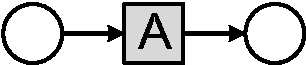
\includegraphics[width=0.3\textwidth]{uniqueness_2_a}
    \end{minipage}
    \begin{minipage}[b]{0.3\textwidth}
      \vspace{1em}
      \centering
      \begin{tabular}{|c|c|c|c|} \hline
        $\rightarrow$ & $\bm{S}$ & $A$ & $\bm{E}$\\ \hline
        $\bm{S}$ & $\overset{\text{\tiny{N}}}{\rightarrow}$ & $\overset{\text{\tiny{DA}}}{\rightarrow}$ & $\overset{\text{\tiny{IA}}}{\rightarrow}$\\ \hline
        $A$ & $\overset{\text{\tiny{N}}}{\rightarrow}$ & $\overset{\text{\tiny{N}}}{\rightarrow}$ & $\overset{\text{\tiny{DA}}}{\rightarrow}$\\ \hline
        $\bm{E}$ & $\overset{\text{\tiny{N}}}{\rightarrow}$ & $\overset{\text{\tiny{N}}}{\rightarrow}$ & $\overset{\text{\tiny{N}}}{\rightarrow}$\\ \hline
      \end{tabular}
    \end{minipage}
    \begin{minipage}[b]{0.3\textwidth}
      \vspace{1em}
      \centering
      \begin{tabular}{|c|c|c|c|} \hline
        $\leftarrow$ & $\bm{S}$ & $A$ & $\bm{E}$\\ \hline
        $\bm{S}$ & $\overset{\text{\tiny{N}}}{\leftarrow}$ & $\overset{\text{\tiny{N}}}{\leftarrow}$ & $\overset{\text{\tiny{N}}}{\leftarrow}$\\ \hline
        $A$ & $\overset{\text{\tiny{DA}}}{\leftarrow}$ & $\overset{\text{\tiny{N}}}{\leftarrow}$ & $\overset{\text{\tiny{N}}}{\leftarrow}$\\ \hline
        $\bm{E}$ & $\overset{\text{\tiny{IA}}}{\leftarrow}$ & $\overset{\text{\tiny{DA}}}{\leftarrow}$ & $\overset{\text{\tiny{N}}}{\leftarrow}$\\ \hline
      \end{tabular}
    \end{minipage}
    \begin{minipage}[b]{0.3\textwidth}
      \vspace{1em}
      \centering
      \begin{tabular}{|c|c|c|c|} \hline
        $\parallel$ & $\bm{S}$ & $A$ & $\bm{E}$\\ \hline
        $\bm{S}$ & $\nparallel$ & $\nparallel$ & $\nparallel$\\ \hline
        $A$ & $\nparallel$ & $\nparallel$ & $\nparallel$\\ \hline
        $\bm{E}$ & $\nparallel$ & $\nparallel$ & $\nparallel$\\ \hline
      \end{tabular}
    \end{minipage}
    \caption{原始部分模型,只含有可见变迁$A$}
    \label{fig:uniqueness_2_a}
  \end{subfigure}

  \begin{subfigure}{1\textwidth}
    \vspace{1em}
    \centering
    \begin{minipage}[b]{1\textwidth}
      \centering
      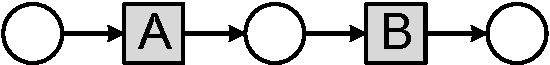
\includegraphics[width=0.5\textwidth]{uniqueness_2_b}
    \end{minipage}
    \begin{minipage}[b]{0.3\textwidth}
      \vspace{1em}
      \centering
      \begin{tabular}{|c|c|c|c|c|} \hline
        $\rightarrow$ & $\bm{S}$ & $A$ & $B$ & $\bm{E}$\\ \hline
        $\bm{S}$ & $\overset{\text{\tiny{N}}}{\rightarrow}$ & $\overset{\text{\tiny{DA}}}{\rightarrow}$ & $\overset{\text{\tiny{IA}}}{\rightarrow}$ & $\overset{\text{\tiny{IA}}}{\rightarrow}$\\ \hline
        $A$ & $\overset{\text{\tiny{N}}}{\rightarrow}$ & $\overset{\text{\tiny{N}}}{\rightarrow}$ & $\overset{\text{\tiny{DA}}}{\rightarrow}$ & $\overset{\text{\tiny{IA}}}{\rightarrow}$\\ \hline
        $B$ & $\overset{\text{\tiny{N}}}{\rightarrow}$ & $\overset{\text{\tiny{N}}}{\rightarrow}$ & $\overset{\text{\tiny{N}}}{\rightarrow}$ & $\overset{\text{\tiny{DA}}}{\rightarrow}$\\ \hline
        $\bm{E}$ & $\overset{\text{\tiny{N}}}{\rightarrow}$ & $\overset{\text{\tiny{N}}}{\rightarrow}$ & $\overset{\text{\tiny{N}}}{\rightarrow}$ & $\overset{\text{\tiny{N}}}{\rightarrow}$\\ \hline
      \end{tabular}
    \end{minipage}
    \begin{minipage}[b]{0.3\textwidth}
      \vspace{1em}
      \centering
      \begin{tabular}{|c|c|c|c|c|} \hline
        $\leftarrow$ & $\bm{S}$ & $A$ & $B$ & $\bm{E}$\\ \hline
        $\bm{S}$ & $\overset{\text{\tiny{N}}}{\leftarrow}$ & $\overset{\text{\tiny{N}}}{\leftarrow}$ & $\overset{\text{\tiny{N}}}{\leftarrow}$ & $\overset{\text{\tiny{N}}}{\leftarrow}$\\ \hline
        $A$ & $\overset{\text{\tiny{DA}}}{\leftarrow}$ & $\overset{\text{\tiny{N}}}{\leftarrow}$ & $\overset{\text{\tiny{N}}}{\leftarrow}$ & $\overset{\text{\tiny{N}}}{\leftarrow}$\\ \hline
        $B$ & $\overset{\text{\tiny{IA}}}{\leftarrow}$ & $\overset{\text{\tiny{DA}}}{\leftarrow}$ & $\overset{\text{\tiny{N}}}{\leftarrow}$ & $\overset{\text{\tiny{N}}}{\leftarrow}$\\ \hline
        $\bm{E}$ & $\overset{\text{\tiny{IA}}}{\leftarrow}$ & $\overset{\text{\tiny{IA}}}{\leftarrow}$ & $\overset{\text{\tiny{DA}}}{\leftarrow}$ & $\overset{\text{\tiny{N}}}{\leftarrow}$\\ \hline
      \end{tabular}
    \end{minipage}
    \begin{minipage}[b]{0.3\textwidth}
      \vspace{1em}
      \centering
      \begin{tabular}{|c|c|c|c|c|} \hline
        $\parallel$ & $\bm{S}$ & $A$ & $B$ & $\bm{E}$\\ \hline
        $\bm{S}$ & $\nparallel$ & $\nparallel$ & $\nparallel$ & $\nparallel$\\ \hline
        $A$ & $\nparallel$ & $\nparallel$ & $\nparallel$ & $\nparallel$\\ \hline
        $B$ & $\nparallel$ & $\nparallel$ & $\nparallel$ & $\nparallel$\\ \hline
        $\bm{E}$ & $\nparallel$ & $\nparallel$ & $\nparallel$ & $\nparallel$\\ \hline
      \end{tabular}
    \end{minipage}
    \caption{在\subref{fig:uniqueness_2_a}中的变迁$A$之后增加一个可见变迁$B$,与$A$同处顺序结构}
    \label{fig:uniqueness_2_b}
  \end{subfigure}

  \begin{subfigure}{1\textwidth}
    \vspace{1em}
    \centering
    \begin{minipage}[b]{1\textwidth}
      \centering
      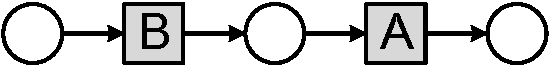
\includegraphics[width=0.5\textwidth]{uniqueness_2_c}
    \end{minipage}
    \begin{minipage}[b]{0.3\textwidth}
      \vspace{1em}
      \centering
      \begin{tabular}{|c|c|c|c|c|} \hline
        $\rightarrow$ & $\bm{S}$ & $A$ & $B$ & $\bm{E}$\\ \hline
        $\bm{S}$ & $\overset{\text{\tiny{N}}}{\rightarrow}$ & $\overset{\text{\tiny{IA}}}{\rightarrow}$ & $\overset{\text{\tiny{DA}}}{\rightarrow}$ & $\overset{\text{\tiny{IA}}}{\rightarrow}$\\ \hline
        $A$ & $\overset{\text{\tiny{N}}}{\rightarrow}$ & $\overset{\text{\tiny{N}}}{\rightarrow}$ & $\overset{\text{\tiny{N}}}{\rightarrow}$ & $\overset{\text{\tiny{DA}}}{\rightarrow}$\\ \hline
        $B$ & $\overset{\text{\tiny{N}}}{\rightarrow}$ & $\overset{\text{\tiny{DA}}}{\rightarrow}$ & $\overset{\text{\tiny{N}}}{\rightarrow}$ & $\overset{\text{\tiny{IA}}}{\rightarrow}$\\ \hline
        $\bm{E}$ & $\overset{\text{\tiny{N}}}{\rightarrow}$ & $\overset{\text{\tiny{N}}}{\rightarrow}$ & $\overset{\text{\tiny{N}}}{\rightarrow}$ & $\overset{\text{\tiny{N}}}{\rightarrow}$\\ \hline
      \end{tabular}
    \end{minipage}
    \begin{minipage}[b]{0.3\textwidth}
      \vspace{1em}
      \centering
      \begin{tabular}{|c|c|c|c|c|} \hline
        $\leftarrow$ & $\bm{S}$ & $A$ & $B$ & $\bm{E}$\\ \hline
        $\bm{S}$ & $\overset{\text{\tiny{N}}}{\leftarrow}$ & $\overset{\text{\tiny{N}}}{\leftarrow}$ & $\overset{\text{\tiny{N}}}{\leftarrow}$ & $\overset{\text{\tiny{N}}}{\leftarrow}$\\ \hline
        $A$ & $\overset{\text{\tiny{IA}}}{\leftarrow}$ & $\overset{\text{\tiny{N}}}{\leftarrow}$ & $\overset{\text{\tiny{DA}}}{\leftarrow}$ & $\overset{\text{\tiny{N}}}{\leftarrow}$\\ \hline
        $B$ & $\overset{\text{\tiny{DA}}}{\leftarrow}$ & $\overset{\text{\tiny{N}}}{\leftarrow}$ & $\overset{\text{\tiny{N}}}{\leftarrow}$ & $\overset{\text{\tiny{N}}}{\leftarrow}$\\ \hline
        $\bm{E}$ & $\overset{\text{\tiny{IA}}}{\leftarrow}$ & $\overset{\text{\tiny{DA}}}{\leftarrow}$ & $\overset{\text{\tiny{IA}}}{\leftarrow}$ & $\overset{\text{\tiny{N}}}{\leftarrow}$\\ \hline
      \end{tabular}
    \end{minipage}
    \begin{minipage}[b]{0.3\textwidth}
      \vspace{1em}
      \centering
      \begin{tabular}{|c|c|c|c|c|} \hline
        $\parallel$ & $\bm{S}$ & $A$ & $B$ & $\bm{E}$\\ \hline
        $\bm{S}$ & $\nparallel$ & $\nparallel$ & $\nparallel$ & $\nparallel$\\ \hline
        $A$ & $\nparallel$ & $\nparallel$ & $\nparallel$ & $\nparallel$\\ \hline
        $B$ & $\nparallel$ & $\nparallel$ & $\nparallel$ & $\nparallel$\\ \hline
        $\bm{E}$ & $\nparallel$ & $\nparallel$ & $\nparallel$ & $\nparallel$\\ \hline
      \end{tabular}
    \end{minipage}
    \caption{在\subref{fig:uniqueness_2_a}中的变迁$A$之前增加一个可见变迁$B$,与$A$同处顺序结构}
    \label{fig:uniqueness_2_c}
  \end{subfigure}

  \begin{subfigure}{1\textwidth}
    \vspace{1em}
    \centering
    \begin{minipage}[b]{1\textwidth}
      \centering
      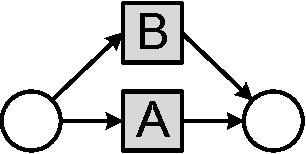
\includegraphics[width=0.3\textwidth]{uniqueness_2_d}
    \end{minipage}
    \begin{minipage}[b]{0.3\textwidth}
      \vspace{1em}
      \centering
      \begin{tabular}{|c|c|c|c|c|} \hline
        $\rightarrow$ & $\bm{S}$ & $A$ & $B$ & $\bm{E}$\\ \hline
        $\bm{S}$ & $\overset{\text{\tiny{N}}}{\rightarrow}$ & $\overset{\text{\tiny{DS}}}{\rightarrow}$ & $\overset{\text{\tiny{DS}}}{\rightarrow}$ & $\overset{\text{\tiny{IA}}}{\rightarrow}$\\ \hline
        $A$ & $\overset{\text{\tiny{N}}}{\rightarrow}$ & $\overset{\text{\tiny{N}}}{\rightarrow}$ & $\overset{\text{\tiny{N}}}{\rightarrow}$ & $\overset{\text{\tiny{DA}}}{\rightarrow}$\\ \hline
        $B$ & $\overset{\text{\tiny{N}}}{\rightarrow}$ & $\overset{\text{\tiny{N}}}{\rightarrow}$ & $\overset{\text{\tiny{N}}}{\rightarrow}$ & $\overset{\text{\tiny{DA}}}{\rightarrow}$\\ \hline
        $\bm{E}$ & $\overset{\text{\tiny{N}}}{\rightarrow}$ & $\overset{\text{\tiny{N}}}{\rightarrow}$ & $\overset{\text{\tiny{N}}}{\rightarrow}$ & $\overset{\text{\tiny{N}}}{\rightarrow}$\\ \hline
      \end{tabular}
    \end{minipage}
    \begin{minipage}[b]{0.3\textwidth}
      \vspace{1em}
      \centering
      \begin{tabular}{|c|c|c|c|c|} \hline
        $\leftarrow$ & $\bm{S}$ & $A$ & $B$ & $\bm{E}$\\ \hline
        $\bm{S}$ & $\overset{\text{\tiny{N}}}{\leftarrow}$ & $\overset{\text{\tiny{N}}}{\leftarrow}$ & $\overset{\text{\tiny{N}}}{\leftarrow}$ & $\overset{\text{\tiny{N}}}{\leftarrow}$\\ \hline
        $A$ & $\overset{\text{\tiny{DA}}}{\leftarrow}$ & $\overset{\text{\tiny{N}}}{\leftarrow}$ & $\overset{\text{\tiny{N}}}{\leftarrow}$ & $\overset{\text{\tiny{N}}}{\leftarrow}$\\ \hline
        $B$ & $\overset{\text{\tiny{DA}}}{\leftarrow}$ & $\overset{\text{\tiny{N}}}{\leftarrow}$ & $\overset{\text{\tiny{N}}}{\leftarrow}$ & $\overset{\text{\tiny{N}}}{\leftarrow}$\\ \hline
        $\bm{E}$ & $\overset{\text{\tiny{IA}}}{\leftarrow}$ & $\overset{\text{\tiny{DS}}}{\leftarrow}$ & $\overset{\text{\tiny{DS}}}{\leftarrow}$ & $\overset{\text{\tiny{N}}}{\leftarrow}$\\ \hline
      \end{tabular}
    \end{minipage}
    \begin{minipage}[b]{0.3\textwidth}
      \vspace{1em}
      \centering
      \begin{tabular}{|c|c|c|c|c|} \hline
        $\parallel$ & $\bm{S}$ & $A$ & $B$ & $\bm{E}$\\ \hline
        $\bm{S}$ & $\nparallel$ & $\nparallel$ & $\nparallel$ & $\nparallel$\\ \hline
        $A$ & $\nparallel$ & $\nparallel$ & $\nparallel$ & $\nparallel$\\ \hline
        $B$ & $\nparallel$ & $\nparallel$ & $\nparallel$ & $\nparallel$\\ \hline
        $\bm{E}$ & $\nparallel$ & $\nparallel$ & $\nparallel$ & $\nparallel$\\ \hline
      \end{tabular}
    \end{minipage}
    \caption{在\subref{fig:uniqueness_2_a}中增加一个可见变迁$B$,与$A$同处互斥结构}
    \label{fig:uniqueness_2_d}
  \end{subfigure}
  \vspace{6pt}
  \caption{向原始模型增加一个可见变迁}
\end{figure}

\begin{figure}[htbp]\ContinuedFloat
  \centering
  \begin{subfigure}{1\textwidth}
    \centering
    \begin{minipage}[b]{1\textwidth}
      \centering
      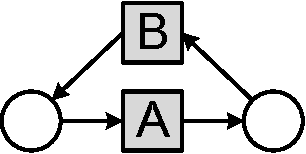
\includegraphics[width=0.3\textwidth]{uniqueness_2_e}
    \end{minipage}
    \begin{minipage}[b]{0.3\textwidth}
      \vspace{1em}
      \centering
      \begin{tabular}{|c|c|c|c|c|} \hline
        $\rightarrow$ & $\bm{S}$ & $A$ & $B$ & $\bm{E}$\\ \hline
        $\bm{S}$ & $\overset{\text{\tiny{N}}}{\rightarrow}$ & $\overset{\text{\tiny{DA}}}{\rightarrow}$ & $\overset{\text{\tiny{IS}}}{\rightarrow}$ & $\overset{\text{\tiny{IA}}}{\rightarrow}$\\ \hline
        $A$ & $\overset{\text{\tiny{N}}}{\rightarrow}$ & $\overset{\text{\tiny{IS}}}{\rightarrow}$ & $\overset{\text{\tiny{DS}}}{\rightarrow}$ & $\overset{\text{\tiny{DS}}}{\rightarrow}$\\ \hline
        $B$ & $\overset{\text{\tiny{N}}}{\rightarrow}$ & $\overset{\text{\tiny{DA}}}{\rightarrow}$ & $\overset{\text{\tiny{IS}}}{\rightarrow}$ & $\overset{\text{\tiny{IS}}}{\rightarrow}$\\ \hline
        $\bm{E}$ & $\overset{\text{\tiny{N}}}{\rightarrow}$ & $\overset{\text{\tiny{N}}}{\rightarrow}$ & $\overset{\text{\tiny{N}}}{\rightarrow}$ & $\overset{\text{\tiny{N}}}{\rightarrow}$\\ \hline
      \end{tabular}
    \end{minipage}
    \begin{minipage}[b]{0.3\textwidth}
      \vspace{1em}
      \centering
      \begin{tabular}{|c|c|c|c|c|} \hline
        $\leftarrow$ & $\bm{S}$ & $A$ & $B$ & $\bm{E}$\\ \hline
        $\bm{S}$ & $\overset{\text{\tiny{N}}}{\leftarrow}$ & $\overset{\text{\tiny{N}}}{\leftarrow}$ & $\overset{\text{\tiny{N}}}{\leftarrow}$ & $\overset{\text{\tiny{N}}}{\leftarrow}$\\ \hline
        $A$ & $\overset{\text{\tiny{DS}}}{\leftarrow}$ & $\overset{\text{\tiny{IS}}}{\leftarrow}$ & $\overset{\text{\tiny{DS}}}{\leftarrow}$ & $\overset{\text{\tiny{N}}}{\leftarrow}$\\ \hline
        $B$ & $\overset{\text{\tiny{IS}}}{\leftarrow}$ & $\overset{\text{\tiny{DA}}}{\leftarrow}$ & $\overset{\text{\tiny{IS}}}{\leftarrow}$ & $\overset{\text{\tiny{N}}}{\leftarrow}$\\ \hline
        $\bm{E}$ & $\overset{\text{\tiny{IA}}}{\leftarrow}$ & $\overset{\text{\tiny{DA}}}{\leftarrow}$ & $\overset{\text{\tiny{IS}}}{\leftarrow}$ & $\overset{\text{\tiny{N}}}{\leftarrow}$\\ \hline
      \end{tabular}
    \end{minipage}
    \begin{minipage}[b]{0.3\textwidth}
      \vspace{1em}
      \centering
      \begin{tabular}{|c|c|c|c|c|} \hline
        $\parallel$ & $\bm{S}$ & $A$ & $B$ & $\bm{E}$\\ \hline
        $\bm{S}$ & $\nparallel$ & $\nparallel$ & $\nparallel$ & $\nparallel$\\ \hline
        $A$ & $\nparallel$ & $\nparallel$ & $\nparallel$ & $\nparallel$\\ \hline
        $B$ & $\nparallel$ & $\nparallel$ & $\nparallel$ & $\nparallel$\\ \hline
        $\bm{E}$ & $\nparallel$ & $\nparallel$ & $\nparallel$ & $\nparallel$\\ \hline
      \end{tabular}
    \end{minipage}
    \caption{在\subref{fig:uniqueness_2_a}中增加一个可见变迁$B$,与$A$同处循环结构}
    \label{fig:uniqueness_2_e}
  \end{subfigure}

  \begin{subfigure}{1\textwidth}
    \vspace{1em}
    \centering
    \begin{minipage}[b]{1\textwidth}
      \centering
      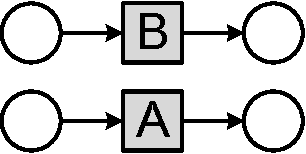
\includegraphics[width=0.3\textwidth]{uniqueness_2_f}
    \end{minipage}
    \begin{minipage}[b]{0.3\textwidth}
      \vspace{1em}
      \centering
      \begin{tabular}{|c|c|c|c|c|} \hline
        $\rightarrow$ & $\bm{S}$ & $A$ & $B$ & $\bm{E}$\\ \hline
        $\bm{S}$ & $\overset{\text{\tiny{N}}}{\rightarrow}$ & $\overset{\text{\tiny{DA}}}{\rightarrow}$ & $\overset{\text{\tiny{DA}}}{\rightarrow}$ & $\overset{\text{\tiny{IA}}}{\rightarrow}$\\ \hline
        $A$ & $\overset{\text{\tiny{N}}}{\rightarrow}$ & $\overset{\text{\tiny{N}}}{\rightarrow}$ & $\overset{\text{\tiny{N}}}{\rightarrow}$ & $\overset{\text{\tiny{DA}}}{\rightarrow}$\\ \hline
        $B$ & $\overset{\text{\tiny{N}}}{\rightarrow}$ & $\overset{\text{\tiny{N}}}{\rightarrow}$ & $\overset{\text{\tiny{N}}}{\rightarrow}$ & $\overset{\text{\tiny{DA}}}{\rightarrow}$\\ \hline
        $\bm{E}$ & $\overset{\text{\tiny{N}}}{\rightarrow}$ & $\overset{\text{\tiny{N}}}{\rightarrow}$ & $\overset{\text{\tiny{N}}}{\rightarrow}$ & $\overset{\text{\tiny{N}}}{\rightarrow}$\\ \hline
      \end{tabular}
    \end{minipage}
    \begin{minipage}[b]{0.3\textwidth}
      \vspace{1em}
      \centering
      \begin{tabular}{|c|c|c|c|c|} \hline
        $\leftarrow$ & $\bm{S}$ & $A$ & $B$ & $\bm{E}$\\ \hline
        $\bm{S}$ & $\overset{\text{\tiny{N}}}{\leftarrow}$ & $\overset{\text{\tiny{N}}}{\leftarrow}$ & $\overset{\text{\tiny{N}}}{\leftarrow}$ & $\overset{\text{\tiny{N}}}{\leftarrow}$\\ \hline
        $A$ & $\overset{\text{\tiny{DA}}}{\leftarrow}$ & $\overset{\text{\tiny{N}}}{\leftarrow}$ & $\overset{\text{\tiny{N}}}{\leftarrow}$ & $\overset{\text{\tiny{N}}}{\leftarrow}$\\ \hline
        $B$ & $\overset{\text{\tiny{DA}}}{\leftarrow}$ & $\overset{\text{\tiny{N}}}{\leftarrow}$ & $\overset{\text{\tiny{N}}}{\leftarrow}$ & $\overset{\text{\tiny{N}}}{\leftarrow}$\\ \hline
        $\bm{E}$ & $\overset{\text{\tiny{IA}}}{\leftarrow}$ & $\overset{\text{\tiny{DA}}}{\leftarrow}$ & $\overset{\text{\tiny{DA}}}{\leftarrow}$ & $\overset{\text{\tiny{N}}}{\leftarrow}$\\ \hline
      \end{tabular}
    \end{minipage}
    \begin{minipage}[b]{0.3\textwidth}
      \vspace{1em}
      \centering
      \begin{tabular}{|c|c|c|c|c|} \hline
        $\parallel$ & $\bm{S}$ & $A$ & $B$ & $\bm{E}$\\ \hline
        $\bm{S}$ & $\nparallel$ & $\nparallel$ & $\nparallel$ & $\nparallel$\\ \hline
        $A$ & $\nparallel$ & $\nparallel$ & $\Updownarrow$ & $\nparallel$\\ \hline
        $B$ & $\nparallel$ & $\Updownarrow$ & $\nparallel$ & $\nparallel$\\ \hline
        $\bm{E}$ & $\nparallel$ & $\nparallel$ & $\nparallel$ & $\nparallel$\\ \hline
      \end{tabular}
    \end{minipage}
    \caption{在\subref{fig:uniqueness_2_a}中增加一个可见变迁$B$,与$A$同处并行结构}
    \label{fig:uniqueness_2_f}
  \end{subfigure}
%     \caption{向原始模型增加一个可见变迁}
% \end{figure}

% \begin{figure}[htbp]\ContinuedFloat
%   \centering
  \vspace{6pt}
  \caption{向原始模型增加一个可见变迁(续)}
  \label{fig:uniqueness_2}
\end{figure}

\begin{figure}[htbp]
  \centering

  \begin{subfigure}{1\textwidth}
    \centering
    \begin{minipage}[b]{1\textwidth}
      \centering
      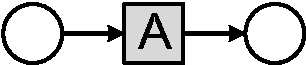
\includegraphics[width=0.3\textwidth]{uniqueness_3_a}
    \end{minipage}
    \begin{minipage}[b]{0.3\textwidth}
      \vspace{1em}
      \centering
      \begin{tabular}{|c|c|c|c|} \hline
        $\rightarrow$ & $\bm{S}$ & $A$ & $\bm{E}$\\ \hline
        $\bm{S}$ & $\overset{\text{\tiny{N}}}{\rightarrow}$ & $\overset{\text{\tiny{DA}}}{\rightarrow}$ & $\overset{\text{\tiny{IA}}}{\rightarrow}$\\ \hline
        $A$ & $\overset{\text{\tiny{N}}}{\rightarrow}$ & $\overset{\text{\tiny{N}}}{\rightarrow}$ & $\overset{\text{\tiny{DA}}}{\rightarrow}$\\ \hline
        $\bm{E}$ & $\overset{\text{\tiny{N}}}{\rightarrow}$ & $\overset{\text{\tiny{N}}}{\rightarrow}$ & $\overset{\text{\tiny{N}}}{\rightarrow}$\\ \hline
      \end{tabular}
    \end{minipage}
    \begin{minipage}[b]{0.3\textwidth}
      \vspace{1em}
      \centering
      \begin{tabular}{|c|c|c|c|} \hline
        $\leftarrow$ & $\bm{S}$ & $A$ & $\bm{E}$\\ \hline
        $\bm{S}$ & $\overset{\text{\tiny{N}}}{\leftarrow}$ & $\overset{\text{\tiny{N}}}{\leftarrow}$ & $\overset{\text{\tiny{N}}}{\leftarrow}$\\ \hline
        $A$ & $\overset{\text{\tiny{DA}}}{\leftarrow}$ & $\overset{\text{\tiny{N}}}{\leftarrow}$ & $\overset{\text{\tiny{N}}}{\leftarrow}$\\ \hline
        $\bm{E}$ & $\overset{\text{\tiny{IA}}}{\leftarrow}$ & $\overset{\text{\tiny{DA}}}{\leftarrow}$ & $\overset{\text{\tiny{N}}}{\leftarrow}$\\ \hline
      \end{tabular}
    \end{minipage}
    \begin{minipage}[b]{0.3\textwidth}
      \vspace{1em}
      \centering
      \begin{tabular}{|c|c|c|c|} \hline
        $\parallel$ & $\bm{S}$ & $A$ & $\bm{E}$\\ \hline
        $\bm{S}$ & $\nparallel$ & $\nparallel$ & $\nparallel$\\ \hline
        $A$ & $\nparallel$ & $\nparallel$ & $\nparallel$\\ \hline
        $\bm{E}$ & $\nparallel$ & $\nparallel$ & $\nparallel$\\ \hline
      \end{tabular}
    \end{minipage}
    \caption{原始部分模型,只含有可见变迁$A$}
    \label{fig:uniqueness_3_a}
  \end{subfigure}
  \vspace{6pt}
  \caption{向原始模型增加一个不可见变迁}
\end{figure}

\begin{figure}[htbp]\ContinuedFloat
  \centering
  \begin{subfigure}{1\textwidth}
    \centering
    \begin{minipage}[b]{1\textwidth}
      \centering
      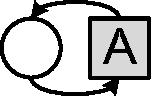
\includegraphics[width=0.11\textwidth]{uniqueness_3_b}
    \end{minipage}
    \begin{minipage}[b]{0.3\textwidth}
      \vspace{1em}
      \centering
      \begin{tabular}{|c|c|c|c|} \hline
        $\rightarrow$ & $\bm{S}$ & $A$ & $\bm{E}$\\ \hline
        $\bm{S}$ & $\overset{\text{\tiny{N}}}{\rightarrow}$ & $\overset{\text{\tiny{DS}}}{\rightarrow}$ & $\overset{\text{\tiny{DA}}}{\rightarrow}$\\ \hline
        $A$ & $\overset{\text{\tiny{N}}}{\rightarrow}$ & $\overset{\text{\tiny{DS}}}{\rightarrow}$ & $\overset{\text{\tiny{DS}}}{\rightarrow}$\\ \hline
        $\bm{E}$ & $\overset{\text{\tiny{N}}}{\rightarrow}$ & $\overset{\text{\tiny{N}}}{\rightarrow}$ & $\overset{\text{\tiny{N}}}{\rightarrow}$\\ \hline
      \end{tabular}
    \end{minipage}
    \begin{minipage}[b]{0.3\textwidth}
      \vspace{1em}
      \centering
      \begin{tabular}{|c|c|c|c|} \hline
        $\leftarrow$ & $\bm{S}$ & $A$ & $\bm{E}$\\ \hline
        $\bm{S}$ & $\overset{\text{\tiny{N}}}{\leftarrow}$ & $\overset{\text{\tiny{N}}}{\leftarrow}$ & $\overset{\text{\tiny{N}}}{\leftarrow}$\\ \hline
        $A$ & $\overset{\text{\tiny{DA}}}{\leftarrow}$ & $\overset{\text{\tiny{DS}}}{\leftarrow}$ & $\overset{\text{\tiny{N}}}{\leftarrow}$\\ \hline
        $\bm{E}$ & $\overset{\text{\tiny{DA}}}{\leftarrow}$ & $\overset{\text{\tiny{DS}}}{\leftarrow}$ & $\overset{\text{\tiny{N}}}{\leftarrow}$\\ \hline
      \end{tabular}
    \end{minipage}
    \begin{minipage}[b]{0.3\textwidth}
      \vspace{1em}
      \centering
      \begin{tabular}{|c|c|c|c|} \hline
        $\parallel$ & $\bm{S}$ & $A$ & $\bm{E}$\\ \hline
        $\bm{S}$ & $\nparallel$ & $\nparallel$ & $\nparallel$\\ \hline
        $A$ & $\nparallel$ & $\nparallel$ & $\nparallel$\\ \hline
        $\bm{E}$ & $\nparallel$ & $\nparallel$ & $\nparallel$\\ \hline
      \end{tabular}
    \end{minipage}
    \caption{将\subref{fig:uniqueness_3_a}中的两个库所合并成一个库所}
    \label{fig:uniqueness_3_b}
  \end{subfigure}

  \begin{subfigure}{1\textwidth}
    \vspace{1em}
    \centering
    \begin{minipage}[b]{1\textwidth}
      \centering
      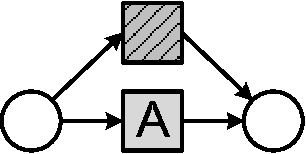
\includegraphics[width=0.3\textwidth]{uniqueness_3_c}
    \end{minipage}
    \begin{minipage}[b]{0.3\textwidth}
      \vspace{1em}
      \centering
      \begin{tabular}{|c|c|c|c|} \hline
        $\rightarrow$ & $\bm{S}$ & $A$ & $\bm{E}$\\ \hline
        $\bm{S}$ & $\overset{\text{\tiny{N}}}{\rightarrow}$ & $\overset{\text{\tiny{DS}}}{\rightarrow}$ & $\overset{\text{\tiny{DA}}}{\rightarrow}$\\ \hline
        $A$ & $\overset{\text{\tiny{N}}}{\rightarrow}$ & $\overset{\text{\tiny{N}}}{\rightarrow}$ & $\overset{\text{\tiny{DA}}}{\rightarrow}$\\ \hline
        $\bm{E}$ & $\overset{\text{\tiny{N}}}{\rightarrow}$ & $\overset{\text{\tiny{N}}}{\rightarrow}$ & $\overset{\text{\tiny{N}}}{\rightarrow}$\\ \hline
      \end{tabular}
    \end{minipage}
    \begin{minipage}[b]{0.3\textwidth}
      \vspace{1em}
      \centering
      \begin{tabular}{|c|c|c|c|} \hline
        $\leftarrow$ & $\bm{S}$ & $A$ & $\bm{E}$\\ \hline
        $\bm{S}$ & $\overset{\text{\tiny{N}}}{\leftarrow}$ & $\overset{\text{\tiny{N}}}{\leftarrow}$ & $\overset{\text{\tiny{N}}}{\leftarrow}$\\ \hline
        $A$ & $\overset{\text{\tiny{DA}}}{\leftarrow}$ & $\overset{\text{\tiny{N}}}{\leftarrow}$ & $\overset{\text{\tiny{N}}}{\leftarrow}$\\ \hline
        $\bm{E}$ & $\overset{\text{\tiny{DA}}}{\leftarrow}$ & $\overset{\text{\tiny{DS}}}{\leftarrow}$ & $\overset{\text{\tiny{N}}}{\leftarrow}$\\ \hline
      \end{tabular}
    \end{minipage}
    \begin{minipage}[b]{0.3\textwidth}
      \vspace{1em}
      \centering
      \begin{tabular}{|c|c|c|c|} \hline
        $\parallel$ & $\bm{S}$ & $A$ & $\bm{E}$\\ \hline
        $\bm{S}$ & $\nparallel$ & $\nparallel$ & $\nparallel$\\ \hline
        $A$ & $\nparallel$ & $\nparallel$ & $\nparallel$\\ \hline
        $\bm{E}$ & $\nparallel$ & $\nparallel$ & $\nparallel$\\ \hline
      \end{tabular}
    \end{minipage}
    \caption{在\subref{fig:uniqueness_3_a}中增加一个不可见变迁,与$A$同处互斥结构}
    \label{fig:uniqueness_3_c}
  \end{subfigure}

  \begin{subfigure}{1\textwidth}
    \vspace{1em}
    \centering
    \begin{minipage}[b]{1\textwidth}
      \centering
      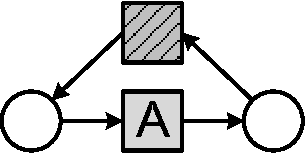
\includegraphics[width=0.3\textwidth]{uniqueness_3_d}
    \end{minipage}
    \begin{minipage}[b]{0.3\textwidth}
      \vspace{1em}
      \centering
      \begin{tabular}{|c|c|c|c|} \hline
        $\rightarrow$ & $\bm{S}$ & $A$ & $\bm{E}$\\ \hline
        $\bm{S}$ & $\overset{\text{\tiny{N}}}{\rightarrow}$ & $\overset{\text{\tiny{DA}}}{\rightarrow}$ & $\overset{\text{\tiny{IA}}}{\rightarrow}$\\ \hline
        $A$ & $\overset{\text{\tiny{N}}}{\rightarrow}$ & $\overset{\text{\tiny{DS}}}{\rightarrow}$ & $\overset{\text{\tiny{DS}}}{\rightarrow}$\\ \hline
        $\bm{E}$ & $\overset{\text{\tiny{N}}}{\rightarrow}$ & $\overset{\text{\tiny{N}}}{\rightarrow}$ & $\overset{\text{\tiny{N}}}{\rightarrow}$\\ \hline
      \end{tabular}
    \end{minipage}
    \begin{minipage}[b]{0.3\textwidth}
      \vspace{1em}
      \centering
      \begin{tabular}{|c|c|c|c|} \hline
        $\leftarrow$ & $\bm{S}$ & $A$ & $\bm{E}$\\ \hline
        $\bm{S}$ & $\overset{\text{\tiny{N}}}{\leftarrow}$ & $\overset{\text{\tiny{N}}}{\leftarrow}$ & $\overset{\text{\tiny{N}}}{\leftarrow}$\\ \hline
        $A$ & $\overset{\text{\tiny{DS}}}{\leftarrow}$ & $\overset{\text{\tiny{DS}}}{\leftarrow}$ & $\overset{\text{\tiny{N}}}{\leftarrow}$\\ \hline
        $\bm{E}$ & $\overset{\text{\tiny{IA}}}{\leftarrow}$ & $\overset{\text{\tiny{DA}}}{\leftarrow}$ & $\overset{\text{\tiny{N}}}{\leftarrow}$\\ \hline
      \end{tabular}
    \end{minipage}
    \begin{minipage}[b]{0.3\textwidth}
      \vspace{1em}
      \centering
      \begin{tabular}{|c|c|c|c|} \hline
        $\parallel$ & $\bm{S}$ & $A$ & $\bm{E}$\\ \hline
        $\bm{S}$ & $\nparallel$ & $\nparallel$ & $\nparallel$\\ \hline
        $A$ & $\nparallel$ & $\nparallel$ & $\nparallel$\\ \hline
        $\bm{E}$ & $\nparallel$ & $\nparallel$ & $\nparallel$\\ \hline
      \end{tabular}
    \end{minipage}
    \caption{在\subref{fig:uniqueness_3_a}中增加一个不可见变迁,与$A$同处循环结构}
    \label{fig:uniqueness_3_d}
  \end{subfigure}
  \vspace{6pt}
  \caption{向原始模型增加一个不可见变迁(续)}
\end{figure}

\begin{figure}[htbp]\ContinuedFloat
  \centering
  \begin{subfigure}{1\textwidth}
    \centering
    \begin{minipage}[b]{1\textwidth}
      \centering
      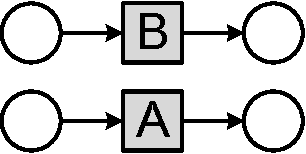
\includegraphics[width=0.3\textwidth]{uniqueness_3_e}
    \end{minipage}
    \begin{minipage}[b]{0.3\textwidth}
      \vspace{1em}
      \centering
      \begin{tabular}{|c|c|c|c|c|} \hline
        $\rightarrow$ & $\bm{S}$ & $A$ & $B$ & $\bm{E}$\\ \hline
        $\bm{S}$ & $\overset{\text{\tiny{N}}}{\rightarrow}$ & $\overset{\text{\tiny{DA}}}{\rightarrow}$ & $\overset{\text{\tiny{DA}}}{\rightarrow}$ & $\overset{\text{\tiny{IA}}}{\rightarrow}$\\ \hline
        $A$ & $\overset{\text{\tiny{N}}}{\rightarrow}$ & $\overset{\text{\tiny{N}}}{\rightarrow}$ & $\overset{\text{\tiny{N}}}{\rightarrow}$ & $\overset{\text{\tiny{DA}}}{\rightarrow}$\\ \hline
        $B$ & $\overset{\text{\tiny{N}}}{\rightarrow}$ & $\overset{\text{\tiny{N}}}{\rightarrow}$ & $\overset{\text{\tiny{N}}}{\rightarrow}$ & $\overset{\text{\tiny{DA}}}{\rightarrow}$\\ \hline
        $\bm{E}$ & $\overset{\text{\tiny{N}}}{\rightarrow}$ & $\overset{\text{\tiny{N}}}{\rightarrow}$ & $\overset{\text{\tiny{N}}}{\rightarrow}$ & $\overset{\text{\tiny{N}}}{\rightarrow}$\\ \hline
      \end{tabular}
    \end{minipage}
    \begin{minipage}[b]{0.3\textwidth}
      \vspace{1em}
      \centering
      \begin{tabular}{|c|c|c|c|c|} \hline
        $\leftarrow$ & $\bm{S}$ & $A$ & $B$ & $\bm{E}$\\ \hline
        $\bm{S}$ & $\overset{\text{\tiny{N}}}{\leftarrow}$ & $\overset{\text{\tiny{N}}}{\leftarrow}$ & $\overset{\text{\tiny{N}}}{\leftarrow}$ & $\overset{\text{\tiny{N}}}{\leftarrow}$\\ \hline
        $A$ & $\overset{\text{\tiny{DA}}}{\leftarrow}$ & $\overset{\text{\tiny{N}}}{\leftarrow}$ & $\overset{\text{\tiny{N}}}{\leftarrow}$ & $\overset{\text{\tiny{N}}}{\leftarrow}$\\ \hline
        $B$ & $\overset{\text{\tiny{DA}}}{\leftarrow}$ & $\overset{\text{\tiny{N}}}{\leftarrow}$ & $\overset{\text{\tiny{N}}}{\leftarrow}$ & $\overset{\text{\tiny{N}}}{\leftarrow}$\\ \hline
        $\bm{E}$ & $\overset{\text{\tiny{IA}}}{\leftarrow}$ & $\overset{\text{\tiny{DA}}}{\leftarrow}$ & $\overset{\text{\tiny{DA}}}{\leftarrow}$ & $\overset{\text{\tiny{N}}}{\leftarrow}$\\ \hline
      \end{tabular}
    \end{minipage}
    \begin{minipage}[b]{0.3\textwidth}
      \vspace{1em}
      \centering
      \begin{tabular}{|c|c|c|c|c|} \hline
        $\parallel$ & $\bm{S}$ & $A$ & $B$ & $\bm{E}$\\ \hline
        $\bm{S}$ & $\nparallel$ & $\nparallel$ & $\nparallel$ & $\nparallel$\\ \hline
        $A$ & $\nparallel$ & $\nparallel$ & $\Updownarrow$ & $\nparallel$\\ \hline
        $B$ & $\nparallel$ & $\Updownarrow$ & $\nparallel$ & $\nparallel$\\ \hline
        $\bm{E}$ & $\nparallel$ & $\nparallel$ & $\nparallel$ & $\nparallel$\\ \hline
      \end{tabular}
    \end{minipage}
    \caption{另一个原始部分模型,含有两个处于并行结构的变迁$A$和变迁$B$}
    \label{fig:uniqueness_3_e}
  \end{subfigure}

  \begin{subfigure}{1\textwidth}
    \vspace{1em}
    \centering
    \begin{minipage}[b]{1\textwidth}
      \centering
      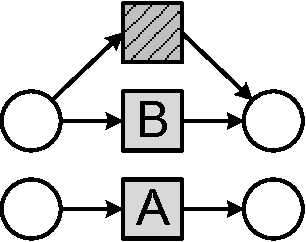
\includegraphics[width=0.3\textwidth]{uniqueness_3_f}
    \end{minipage}
    \begin{minipage}[b]{0.3\textwidth}
      \vspace{1em}
      \centering
      \begin{tabular}{|c|c|c|c|c|} \hline
        $\rightarrow$ & $\bm{S}$ & $A$ & $B$ & $\bm{E}$\\ \hline
        $\bm{S}$ & $\overset{\text{\tiny{N}}}{\rightarrow}$ & $\overset{\text{\tiny{DA}}}{\rightarrow}$ & $\overset{\text{\tiny{DS}}}{\rightarrow}$ & $\overset{\text{\tiny{IA}}}{\rightarrow}$\\ \hline
        $A$ & $\overset{\text{\tiny{N}}}{\rightarrow}$ & $\overset{\text{\tiny{N}}}{\rightarrow}$ & $\overset{\text{\tiny{N}}}{\rightarrow}$ & $\overset{\text{\tiny{DA}}}{\rightarrow}$\\ \hline
        $B$ & $\overset{\text{\tiny{N}}}{\rightarrow}$ & $\overset{\text{\tiny{N}}}{\rightarrow}$ & $\overset{\text{\tiny{N}}}{\rightarrow}$ & $\overset{\text{\tiny{DA}}}{\rightarrow}$\\ \hline
        $\bm{E}$ & $\overset{\text{\tiny{N}}}{\rightarrow}$ & $\overset{\text{\tiny{N}}}{\rightarrow}$ & $\overset{\text{\tiny{N}}}{\rightarrow}$ & $\overset{\text{\tiny{N}}}{\rightarrow}$\\ \hline
      \end{tabular}
    \end{minipage}
    \begin{minipage}[b]{0.3\textwidth}
      \vspace{1em}
      \centering
      \begin{tabular}{|c|c|c|c|c|} \hline
        $\leftarrow$ & $\bm{S}$ & $A$ & $B$ & $\bm{E}$\\ \hline
        $\bm{S}$ & $\overset{\text{\tiny{N}}}{\leftarrow}$ & $\overset{\text{\tiny{N}}}{\leftarrow}$ & $\overset{\text{\tiny{N}}}{\leftarrow}$ & $\overset{\text{\tiny{N}}}{\leftarrow}$\\ \hline
        $A$ & $\overset{\text{\tiny{DA}}}{\leftarrow}$ & $\overset{\text{\tiny{N}}}{\leftarrow}$ & $\overset{\text{\tiny{N}}}{\leftarrow}$ & $\overset{\text{\tiny{N}}}{\leftarrow}$\\ \hline
        $B$ & $\overset{\text{\tiny{DA}}}{\leftarrow}$ & $\overset{\text{\tiny{N}}}{\leftarrow}$ & $\overset{\text{\tiny{N}}}{\leftarrow}$ & $\overset{\text{\tiny{N}}}{\leftarrow}$\\ \hline
        $\bm{E}$ & $\overset{\text{\tiny{IA}}}{\leftarrow}$ & $\overset{\text{\tiny{DA}}}{\leftarrow}$ & $\overset{\text{\tiny{DS}}}{\leftarrow}$ & $\overset{\text{\tiny{N}}}{\leftarrow}$\\ \hline
      \end{tabular}
    \end{minipage}
    \begin{minipage}[b]{0.3\textwidth}
      \vspace{1em}
      \centering
      \begin{tabular}{|c|c|c|c|c|} \hline
        $\parallel$ & $\bm{S}$ & $A$ & $B$ & $\bm{E}$\\ \hline
        $\bm{S}$ & $\nparallel$ & $\nparallel$ & $\nparallel$ & $\nparallel$\\ \hline
        $A$ & $\nparallel$ & $\nparallel$ & $\Uparrow$ & $\nparallel$\\ \hline
        $B$ & $\nparallel$ & $\Updownarrow$ & $\nparallel$ & $\nparallel$\\ \hline
        $\bm{E}$ & $\nparallel$ & $\nparallel$ & $\nparallel$ & $\nparallel$\\ \hline
      \end{tabular}
    \end{minipage}
    \caption{在\subref{fig:uniqueness_3_e}中增加一个不可见变迁,与$B$同处互斥结构}
    \label{fig:uniqueness_3_f}
  \end{subfigure}

  \begin{subfigure}{1\textwidth}
    \vspace{1em}
    \centering
    \begin{minipage}[b]{1\textwidth}
      \centering
      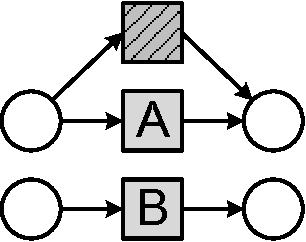
\includegraphics[width=0.3\textwidth]{uniqueness_3_g}
    \end{minipage}
    \begin{minipage}[b]{0.3\textwidth}
      \vspace{1em}
      \centering
      \begin{tabular}{|c|c|c|c|c|} \hline
        $\rightarrow$ & $\bm{S}$ & $A$ & $B$ & $\bm{E}$\\ \hline
        $\bm{S}$ & $\overset{\text{\tiny{N}}}{\rightarrow}$ & $\overset{\text{\tiny{DS}}}{\rightarrow}$ & $\overset{\text{\tiny{DA}}}{\rightarrow}$ & $\overset{\text{\tiny{IA}}}{\rightarrow}$\\ \hline
        $A$ & $\overset{\text{\tiny{N}}}{\rightarrow}$ & $\overset{\text{\tiny{N}}}{\rightarrow}$ & $\overset{\text{\tiny{N}}}{\rightarrow}$ & $\overset{\text{\tiny{DA}}}{\rightarrow}$\\ \hline
        $B$ & $\overset{\text{\tiny{N}}}{\rightarrow}$ & $\overset{\text{\tiny{N}}}{\rightarrow}$ & $\overset{\text{\tiny{N}}}{\rightarrow}$ & $\overset{\text{\tiny{DA}}}{\rightarrow}$\\ \hline
        $\bm{E}$ & $\overset{\text{\tiny{N}}}{\rightarrow}$ & $\overset{\text{\tiny{N}}}{\rightarrow}$ & $\overset{\text{\tiny{N}}}{\rightarrow}$ & $\overset{\text{\tiny{N}}}{\rightarrow}$\\ \hline
      \end{tabular}
    \end{minipage}
    \begin{minipage}[b]{0.3\textwidth}
      \vspace{1em}
      \centering
      \begin{tabular}{|c|c|c|c|c|} \hline
        $\leftarrow$ & $\bm{S}$ & $A$ & $B$ & $\bm{E}$\\ \hline
        $\bm{S}$ & $\overset{\text{\tiny{N}}}{\leftarrow}$ & $\overset{\text{\tiny{N}}}{\leftarrow}$ & $\overset{\text{\tiny{N}}}{\leftarrow}$ & $\overset{\text{\tiny{N}}}{\leftarrow}$\\ \hline
        $A$ & $\overset{\text{\tiny{DA}}}{\leftarrow}$ & $\overset{\text{\tiny{N}}}{\leftarrow}$ & $\overset{\text{\tiny{N}}}{\leftarrow}$ & $\overset{\text{\tiny{N}}}{\leftarrow}$\\ \hline
        $B$ & $\overset{\text{\tiny{DA}}}{\leftarrow}$ & $\overset{\text{\tiny{N}}}{\leftarrow}$ & $\overset{\text{\tiny{N}}}{\leftarrow}$ & $\overset{\text{\tiny{N}}}{\leftarrow}$\\ \hline
        $\bm{E}$ & $\overset{\text{\tiny{IA}}}{\leftarrow}$ & $\overset{\text{\tiny{DS}}}{\leftarrow}$ & $\overset{\text{\tiny{DA}}}{\leftarrow}$ & $\overset{\text{\tiny{N}}}{\leftarrow}$\\ \hline
      \end{tabular}
    \end{minipage}
    \begin{minipage}[b]{0.3\textwidth}
      \vspace{1em}
      \centering
      \begin{tabular}{|c|c|c|c|c|} \hline
        $\parallel$ & $\bm{S}$ & $A$ & $B$ & $\bm{E}$\\ \hline
        $\bm{S}$ & $\nparallel$ & $\nparallel$ & $\nparallel$ & $\nparallel$\\ \hline
        $A$ & $\nparallel$ & $\nparallel$ & $\Updownarrow$ & $\nparallel$\\ \hline
        $B$ & $\nparallel$ & $\Uparrow$ & $\nparallel$ & $\nparallel$\\ \hline
        $\bm{E}$ & $\nparallel$ & $\nparallel$ & $\nparallel$ & $\nparallel$\\ \hline
      \end{tabular}
    \end{minipage}
    \caption{在\subref{fig:uniqueness_3_e}中增加一个不可见变迁,与$A$同处互斥结构}
    \label{fig:uniqueness_3_g}
  \end{subfigure}
  \vspace{6pt}
  \caption{向原始模型增加一个不可见变迁(续)}
\end{figure}

\begin{figure}[htbp]\ContinuedFloat
  \centering
  \begin{subfigure}{1\textwidth}
    \centering
    \begin{minipage}[b]{1\textwidth}
      \centering
      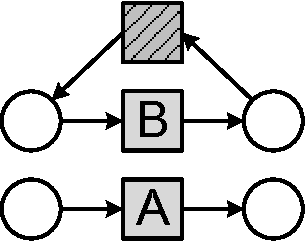
\includegraphics[width=0.3\textwidth]{uniqueness_3_h}
    \end{minipage}
    \begin{minipage}[b]{0.3\textwidth}
      \vspace{1em}
      \centering
      \begin{tabular}{|c|c|c|c|c|} \hline
        $\rightarrow$ & $\bm{S}$ & $A$ & $B$ & $\bm{E}$\\ \hline
        $\bm{S}$ & $\overset{\text{\tiny{N}}}{\rightarrow}$ & $\overset{\text{\tiny{DA}}}{\rightarrow}$ & $\overset{\text{\tiny{DA}}}{\rightarrow}$ & $\overset{\text{\tiny{IA}}}{\rightarrow}$\\ \hline
        $A$ & $\overset{\text{\tiny{N}}}{\rightarrow}$ & $\overset{\text{\tiny{N}}}{\rightarrow}$ & $\overset{\text{\tiny{N}}}{\rightarrow}$ & $\overset{\text{\tiny{DA}}}{\rightarrow}$\\ \hline
        $B$ & $\overset{\text{\tiny{N}}}{\rightarrow}$ & $\overset{\text{\tiny{N}}}{\rightarrow}$ & $\overset{\text{\tiny{DS}}}{\rightarrow}$ & $\overset{\text{\tiny{DS}}}{\rightarrow}$\\ \hline
        $\bm{E}$ & $\overset{\text{\tiny{N}}}{\rightarrow}$ & $\overset{\text{\tiny{N}}}{\rightarrow}$ & $\overset{\text{\tiny{N}}}{\rightarrow}$ & $\overset{\text{\tiny{N}}}{\rightarrow}$\\ \hline
      \end{tabular}
    \end{minipage}
    \begin{minipage}[b]{0.3\textwidth}
      \vspace{1em}
      \centering
      \begin{tabular}{|c|c|c|c|c|} \hline
        $\leftarrow$ & $\bm{S}$ & $A$ & $B$ & $\bm{E}$\\ \hline
        $\bm{S}$ & $\overset{\text{\tiny{N}}}{\leftarrow}$ & $\overset{\text{\tiny{N}}}{\leftarrow}$ & $\overset{\text{\tiny{N}}}{\leftarrow}$ & $\overset{\text{\tiny{N}}}{\leftarrow}$\\ \hline
        $A$ & $\overset{\text{\tiny{DA}}}{\leftarrow}$ & $\overset{\text{\tiny{N}}}{\leftarrow}$ & $\overset{\text{\tiny{N}}}{\leftarrow}$ & $\overset{\text{\tiny{N}}}{\leftarrow}$\\ \hline
        $B$ & $\overset{\text{\tiny{DS}}}{\leftarrow}$ & $\overset{\text{\tiny{N}}}{\leftarrow}$ & $\overset{\text{\tiny{DS}}}{\leftarrow}$ & $\overset{\text{\tiny{N}}}{\leftarrow}$\\ \hline
        $\bm{E}$ & $\overset{\text{\tiny{IA}}}{\leftarrow}$ & $\overset{\text{\tiny{DA}}}{\leftarrow}$ & $\overset{\text{\tiny{DA}}}{\leftarrow}$ & $\overset{\text{\tiny{N}}}{\leftarrow}$\\ \hline
      \end{tabular}
    \end{minipage}
    \begin{minipage}[b]{0.3\textwidth}
      \vspace{1em}
      \centering
      \begin{tabular}{|c|c|c|c|c|} \hline
        $\parallel$ & $\bm{S}$ & $A$ & $B$ & $\bm{E}$\\ \hline
        $\bm{S}$ & $\nparallel$ & $\nparallel$ & $\nparallel$ & $\nparallel$\\ \hline
        $A$ & $\nparallel$ & $\nparallel$ & $\Updownarrow$ & $\nparallel$\\ \hline
        $B$ & $\nparallel$ & $\Uparrow$ & $\nparallel$ & $\nparallel$\\ \hline
        $\bm{E}$ & $\nparallel$ & $\nparallel$ & $\nparallel$ & $\nparallel$\\ \hline
      \end{tabular}
    \end{minipage}
    \caption{在\subref{fig:uniqueness_3_e}中增加一个不可见变迁,与$B$同处循环结构}
    \label{fig:uniqueness_3_h}
  \end{subfigure}

  \begin{subfigure}{1\textwidth}
    \vspace{1em}
    \centering
    \begin{minipage}[b]{1\textwidth}
      \centering
      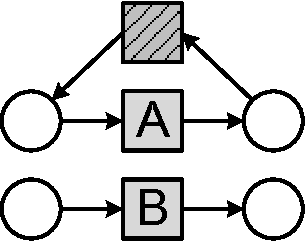
\includegraphics[width=0.3\textwidth]{uniqueness_3_i}
    \end{minipage}
    \begin{minipage}[b]{0.3\textwidth}
      \vspace{1em}
      \centering
      \begin{tabular}{|c|c|c|c|c|} \hline
        $\rightarrow$ & $\bm{S}$ & $A$ & $B$ & $\bm{E}$\\ \hline
        $\bm{S}$ & $\overset{\text{\tiny{N}}}{\rightarrow}$ & $\overset{\text{\tiny{DA}}}{\rightarrow}$ & $\overset{\text{\tiny{DA}}}{\rightarrow}$ & $\overset{\text{\tiny{IA}}}{\rightarrow}$\\ \hline
        $A$ & $\overset{\text{\tiny{N}}}{\rightarrow}$ & $\overset{\text{\tiny{DS}}}{\rightarrow}$ & $\overset{\text{\tiny{N}}}{\rightarrow}$ & $\overset{\text{\tiny{DS}}}{\rightarrow}$\\ \hline
        $B$ & $\overset{\text{\tiny{N}}}{\rightarrow}$ & $\overset{\text{\tiny{N}}}{\rightarrow}$ & $\overset{\text{\tiny{N}}}{\rightarrow}$ & $\overset{\text{\tiny{DA}}}{\rightarrow}$\\ \hline
        $\bm{E}$ & $\overset{\text{\tiny{N}}}{\rightarrow}$ & $\overset{\text{\tiny{N}}}{\rightarrow}$ & $\overset{\text{\tiny{N}}}{\rightarrow}$ & $\overset{\text{\tiny{N}}}{\rightarrow}$\\ \hline
      \end{tabular}
    \end{minipage}
    \begin{minipage}[b]{0.3\textwidth}
      \vspace{1em}
      \centering
      \begin{tabular}{|c|c|c|c|c|} \hline
        $\leftarrow$ & $\bm{S}$ & $A$ & $B$ & $\bm{E}$\\ \hline
        $\bm{S}$ & $\overset{\text{\tiny{N}}}{\leftarrow}$ & $\overset{\text{\tiny{N}}}{\leftarrow}$ & $\overset{\text{\tiny{N}}}{\leftarrow}$ & $\overset{\text{\tiny{N}}}{\leftarrow}$\\ \hline
        $A$ & $\overset{\text{\tiny{DS}}}{\leftarrow}$ & $\overset{\text{\tiny{DS}}}{\leftarrow}$ & $\overset{\text{\tiny{N}}}{\leftarrow}$ & $\overset{\text{\tiny{N}}}{\leftarrow}$\\ \hline
        $B$ & $\overset{\text{\tiny{DA}}}{\leftarrow}$ & $\overset{\text{\tiny{N}}}{\leftarrow}$ & $\overset{\text{\tiny{N}}}{\leftarrow}$ & $\overset{\text{\tiny{N}}}{\leftarrow}$\\ \hline
        $\bm{E}$ & $\overset{\text{\tiny{IA}}}{\leftarrow}$ & $\overset{\text{\tiny{DA}}}{\leftarrow}$ & $\overset{\text{\tiny{DA}}}{\leftarrow}$ & $\overset{\text{\tiny{N}}}{\leftarrow}$\\ \hline
      \end{tabular}
    \end{minipage}
    \begin{minipage}[b]{0.3\textwidth}
      \vspace{1em}
      \centering
      \begin{tabular}{|c|c|c|c|c|} \hline
        $\parallel$ & $\bm{S}$ & $A$ & $B$ & $\bm{E}$\\ \hline
        $\bm{S}$ & $\nparallel$ & $\nparallel$ & $\nparallel$ & $\nparallel$\\ \hline
        $A$ & $\nparallel$ & $\nparallel$ & $\Uparrow$ & $\nparallel$\\ \hline
        $B$ & $\nparallel$ & $\Updownarrow$ & $\nparallel$ & $\nparallel$\\ \hline
        $\bm{E}$ & $\nparallel$ & $\nparallel$ & $\nparallel$ & $\nparallel$\\ \hline
      \end{tabular}
    \end{minipage}
    \caption{在\subref{fig:uniqueness_3_e}中增加一个不可见变迁,与$A$同处循环结构}
    \label{fig:uniqueness_3_i}
  \end{subfigure}
  %     \caption{向原始模型增加一个不可见变迁}
% \end{figure}

% \begin{figure}[htbp]\ContinuedFloat
%   \centering
  \vspace{6pt}
  \caption{向原始模型增加一个不可见变迁(续)}
  \label{fig:uniqueness_3}
\end{figure}
% \end{appendix}

%% 个人简历
\begin{resume}

  \resumeitem{个人简历}

  1992年7月28日出生于江西省贵溪市。

  2009年9月考入清华大学软件学院计算机软件专业,2013年7月本科毕业并获得工学学士学位。

  2013年9月免试进入清华大学软件学院攻读软件工程硕士学位至今。

  \researchitem{发表的学术论文} % 发表的和录用的合在一起

  % 1. 已经刊载的学术论文(本人是第一作者,或者导师为第一作者本人是第二作者)
  \begin{publications}
    \item 汪抒浩, 闻立杰, 魏代森, 等. 基于任务最短跟随距离矩阵的流程模型行为相似性算法[J]. 计算机集成制造系统, 2013, 19(08): 1822-1831.(EI收录,检索号:20133916789912)
    \item Wang S, Yin M, Wang Z, et al. TAR++: A New Process Model Similarity Algorithm Based on the Importance of TARs[M]//Asia Pacific Business Process Management. Springer International Publishing, 2015: 98-112.(EI收录,检索号:20154601556389)
    \item Wang S, Lv C, Wen L, et al. Managing Massive Business Process Models and Instances with Process Space[C]//BPM (Demos). 2014: 91.
  \end{publications}

  % % 2. 尚未刊载,但已经接到正式录用函的学术论文(本人为第一作者,或者
  % %    导师为第一作者本人是第二作者)。
  % \begin{publications}[before=\publicationskip,after=\publicationskip]
  %   \item Yang Y, Ren T L, Zhu Y P, et al. PMUTs for handwriting recognition. In
  %     press. (已被 Integrated Ferroelectrics 录用. SCI 源刊.)
  % \end{publications}

  % % 3. 其他学术论文。可列出除上述两种情况以外的其他学术论文,但必须是
  % %    已经刊载或者收到正式录用函的论文。
  % \begin{publications}
  %   \item Wu X M, Yang Y, Cai J, et al. Measurements of ferroelectric MEMS
  %     microphones. Integrated Ferroelectrics, 2005, 69:417-429. (SCI 收录, 检索号
  %     :896KM)
  %   \item 贾泽, 杨轶, 陈兢, 等. 用于压电和电容微麦克风的体硅腐蚀相关研究. 压电与声
  %     光, 2006, 28(1):117-119. (EI 收录, 检索号:06129773469)
  %   \item 伍晓明, 杨轶, 张宁欣, 等. 基于MEMS技术的集成铁电硅微麦克风. 中国集成电路,
  %     2003, 53:59-61.
  % \end{publications}

  % \researchitem{研究成果} % 有就写,没有就删除
  % \begin{achievements}
  %   \item 任天令, 杨轶, 朱一平, 等. 硅基铁电微声学传感器畴极化区域控制和电极连接的
  %     方法: 中国, CN1602118A. (中国专利公开号)
  %   \item Ren T L, Yang Y, Zhu Y P, et al. Piezoelectric micro acoustic sensor
  %     based on ferroelectric materials: USA, No.11/215, 102. (美国发明专利申请号)
  % \end{achievements}

\end{resume}

\end{document}